\documentclass[a4paper,11pt,notitlepage]{report}

\usepackage{graphicx}
\usepackage[utf8]{inputenc}
\usepackage{libertine}
\renewcommand*\oldstylenums[1]{{\fontfamily{fxlj}\selectfont #1}}
\usepackage[T1]{fontenc}
\usepackage[ngerman]{babel}
\usepackage{bibgerm}
\usepackage{amsmath,amssymb,amsthm}
\usepackage{color}
\usepackage{enumerate}
\usepackage{tabularx}
\usepackage{subfig}
\usepackage{fancyhdr}
\usepackage[pdftex,pdfpagelabels,colorlinks,backref,pagebackref]{hyperref}
\usepackage{tikz} % SELBST HINZUGEFÜGT
\usepackage{diagbox}
% == Set the heading style ===================================================
\setlength{\headheight}{14pt}
\pagestyle{fancyplain}
\renewcommand{\chaptermark}[1]{\markboth{#1}{}}
\renewcommand{\sectionmark}[1]{\markright{\thesection\ #1}}
\lhead[\fancyplain{}{\thepage}]{\fancyplain{}{\rightmark}}
\rhead[\fancyplain{}{\leftmark}]{\fancyplain{}{\thepage}}
\cfoot{}
\renewcommand{\headrulewidth}{0.4pt}
% ============================================================================

% == Set correct values for fitting floats ===================================
\tolerance=2000
\emergencystretch=10pt

\setcounter{topnumber}{3}
\setcounter{totalnumber}{5}
\setcounter{bottomnumber}{2}

% To make those darn floats fit where they should
\setcounter{totalnumber}{9}
\setcounter{topnumber}{9}
\setcounter{bottomnumber}{9}
\renewcommand{\textfraction}{0.00}
\renewcommand{\topfraction}{1.0}
\renewcommand{\bottomfraction}{1.0}
% ============================================================================

% == German definitions for theorems etc. ==================================== 
\newtheorem{definition}{Definition}[chapter]
\newtheorem{theorem}{Satz}[chapter]
\newtheorem{lemma}{Lemma}[chapter]
\newtheorem{proposition}{Proposition}[chapter]
\newtheorem{corollary}{Korollar}[chapter]
\newtheorem{observation}{Beobachtung}[chapter]
\newtheorem{fact}{Fakt}[chapter]
\newtheorem{remark}{Bemerkung}[chapter]
\newtheorem{example}{Beispiel}[chapter]
% ============================================================================

% == Abkürzungen für die reellen, natürlichen, ganzen,... Zahlen =============
\newcommand{\R}{{\ensuremath{\mathbb{R}}}}
\newcommand{\N}{{\ensuremath{\mathbb{N}}}}
\newcommand{\Z}{{\ensuremath{\mathbb{Z}}}}
\newcommand{\C}{{\ensuremath{\mathbb{C}}}}
\newcommand{\Q}{{\ensuremath{\mathbb{Q}}}}
\newcommand{\F}{{\ensuremath{\mathbb{F}}}}
\newcommand{\Prim}{{\ensuremath{\mathbb{P}}}}
\newcommand{\E}{{\ensuremath{\mathbb{E}}}}
% ============================================================================

% == Makros für Autorenname und -adresse =====================================
\newcommand{\myaddress}[6]{%
  \parbox{\textwidth}{\textbf{\large #1}\\
    #2\\ #3\\ #4\\ 
    \ifthenelse{\equal{#5}{}}{}{Email: \href{mailto:#5}{\texttt{#5}}\\}
    \ifthenelse{\equal{#6}{}}{}{WWW: \href{#6}{\path|#6|}\\}
  } 
}

\newcommand{\myauthor}[1]{%
  \addtocontents{toc}{\protect\hspace{3.35ex}%
  \textsl{#1}\par}\vspace{-4ex}\quad\hfill\textsl{\Large #1}\vspace{8ex}}

\newcommand{\myname}[1]{\Large #1}

\title{\textbf{{Einführung in die Stochastik - Mitschrieb} \\[5ex] 
    {\Large Vorlesung im Wintersemester 2011/2012\\[5ex]}}}

%%%%%%%%%%%%%%%%%%%%%%%%%%%%%%%%%%%%%%%%%%%%%%%%%%
% Tragen Sie in der folg. Zeile Ihren Namen ein: %
%%%%%%%%%%%%%%%%%%%%%%%%%%%%%%%%%%%%%%%%%%%%%%%%%%
\author{\myname{Sarah Lutteropp}}

\begin{document}
\shorthandoff{"}
\maketitle
\setcounter{tocdepth}{1}
\tableofcontents

\section*{Vorwort}
Dies ist ein Mitschrieb der Vorlesung “Einführung in die Stochastik” vom Wintersemester 2011/2012 am Karlsruher Institut für Technologie, die von Herrn Prof. Dr. Günther Last gehalten wird.

\chapter{Deskriptive Statistik}
\section{Der Grundraum}
$\emptyset \neq \Omega$ = Grundraum (Grundgesamtheit, Merkmalsraum, Stichprobenraum)
Annahme: $\Omega$ ist diskret(endlich oder abzählbar unendlich) (Häufig $\Omega \subseteq \R$)

\section{Absolute und relative Häufigkeit}
$x_1, \ldots, x_n \in \Omega$ ("Daten") \newline
$h(\omega) = \text{card}\left\{j\in\{1, \ldots, n\} \colon x_j = \omega\right\}, \omega \in \Omega$, absolute Häufigkeit von $\omega$

\paragraph{Bemerkung}
$\sum\limits_{\omega \in \Omega}{h(\omega)} = n$

\paragraph{Definition}
$\frac{1}{n} h(\omega)$ = relative Häufigkeit von $\omega$ \newline
$h(A)=\text{card}\left\{j\in\{1,\ldots,n\}\colon x_j \in A\right\}, A \subset \Omega$ = absolute Häufigkeit von A, $\frac{1}{n} h(A)$ = relative Häufigkeit von A

\section{Histogramm}
$x_1, \ldots, x_n \in \R, b_1 < b_2 < \ldots < b_s$ mit $b_1 \leq \min\limits_{1 \leq i \leq n}{x_i}, b_s > \max\limits_{1 \leq i \leq n}{x_i}$
\newline
TODO: BILD
\newline
$d_j(b_{j+1}-b_j)=h([b_j,b_{j+1})) = \text{card} \left\{i\in\{1,\ldots,n\}\colon b_j \leq x_i < b_{j+1}\right\}$

\section{Lagemaße}
\paragraph{Definition}
Ein \textbf{Lagemaß} ist eine Abbildung $l \colon \R^n \rightarrow \R$ mit $$l(x_1+a,\ldots,x_n+a) = l(x_1,\ldots,x_n)+a$$ "Verschiebungskovarianz".
$x_1,\ldots,x_n,a \in \R$

\subsection{Arithmetisches Mittel}
$x_1,\ldots,x_n \in \R, \bar{x} := \frac{1}{n} \sum\limits_{j=1}^{n}{x_j}$ "Schwerpunkt der Daten"

\paragraph{Fakt}
$\sum\limits_{j=1}^{n}{(x_i - t)^2} \overset{t}{\rightarrow} \text{Min}$
\newline
Lösung: $t = \bar{x}$
\newline
"Prinzip der kleinsten Quadrate"

\paragraph{Beweis}
$\frac{1}{n} \sum\limits_{j=1}^{n}{(x_j - t)^2} = t^2 - 2\bar{x}t + \frac{1}{n} \sum\limits_{j=1}^{n}{x_j^2} = (t - \bar{x})^2 + \frac{1}{n} \sum\limits_{j=1}^{n}{x_j^2 - (\bar{x})^2}$

\subsection{Median, Quantile}
$x_1,\ldots,x_n \in \R \Rightarrow x_{(1)} \leq x_{(2)} \leq \ldots \leq x_{(n)}$ geordnete Stichprobe

\paragraph{Definition}

$$x_{1/2}:= \begin{cases}
	x_{(\frac{n+1}{2})} & \text{, falls } n \text{ ungerade} \\
	\frac{1}{2}(x_{(\frac{n}{2})} + x_{(\frac{n}{2}+1)}) & \text{, falls } n \text{ gerade}
\end{cases}
$$ 
heißt \textbf{Median} von $x_1,\ldots,x_n$.

\paragraph{Fakt}
$\sum\limits_{j=1}^{n}{|x_j - x_{1/2}|} = \min\limits_{t}{\sum\limits_{j=1}^{n}{|x_j - t|}}$ Übungsaufgabe

\paragraph{Bemerkung}
Der Median ist "robust" gegenüber "Ausreißern".
Ist etwa $x_1 = \ldots = x_9 = 1$ und $x_{10} = 1000 (n=10)$, so gilt $\bar{x} = 100,9  , x_{1/2} = 1$

\paragraph{Definition}
Für 0 < p < 1 heißt
$$
x_p := \begin{cases}
	x_{(\lfloor n \cdot p + 1 \rfloor )} & \text{, falls } n \cdot p \notin \N \\
	\frac{1}{2}(x_{(n \cdot p)} + x_{(n \cdot p + 1)}) & \text{, falls } n \cdot p \in \N
\end{cases}
$$
\textbf{p-Quantil} von $x_1, \ldots, x_n$.

\paragraph{Interpretation}
Mindestens $p \cdot 100 \%$ der Daten liegen links von $x_p$ und mindestens $(1-p) \cdot 100 \%$ liegen rechts von $x_p$. \newline
$x_{1/4}=$ unteres Quartil, $x_{3/4}=$ oberes Quartil

\section{Streuungsmaße}
\paragraph{Definition}
Eine Abbildung $\sigma \colon \R^n \rightarrow \R$ mit $$\sigma(x_1+a,\ldots,x_n+a) = \sigma(x_1,\ldots,x_n)\text{ (Translationsinvarianz)}$$ heißt \textbf{Streuungsmaß}.

\subsection{Empirische Varianz}
$s^2 := \frac{1}{n-1} \sum\limits_{j=1}^{n}{(x_j - \bar{x})^2}$ = \textbf{empirische Varianz} von $x_1,\ldots,x_n$

\subsection{Empirische Standardabweichung}
$s := + \sqrt{s^2}$ = \textbf{empirische Standardabweichung} von $x_1,\ldots,x_n$

\subsection{Spannweite}
$x_{(n)} - x_{(1)}$ = \textbf{Spannweite} von $x_1,\ldots,x_n$

\subsection{Quartilsabstand}
$x_{(3/4)} - x_{(1/4)}$ = \textbf{Quartilsabstand} von $x_1,\ldots,x_n$

\section{Empirischer Korrelationskoeffizient}

$(x_1,y_1), \ldots, (x_n,y_n) \in \R^2$
TODO: BILD

Gesucht: Gerade $y = a + b \cdot x$ so, dass
$$(*) \sum\limits_{j=1}^{n}{(y_j - a - b x_j)^2} \overset{a,b}\rightarrow \text{Min}$$

\paragraph{Definition}
$\sigma_{x}^2 = \frac{1}{n}\sum\limits_{j=1}^{n}{(x_j - \bar{x})^2}$
$\sigma_{y}^2 = \frac{1}{n}\sum\limits_{j=1}^{n}{(y_j - \bar{y})^2}$

$\sigma_{xy} = \frac{1}{n}\sum\limits_{j=1}^{n}{(x_j - \bar{x})(y_j - \bar{y})}$ \textbf{empirische Kovarianz} $\sigma_x^2 > 0, \sigma_y^2 >0.$

Lösung von (*):
$b^* = \frac{\sigma_{xy}}{\sigma_{x^2}}, a^*= \bar{y} - b^* \cdot \bar{x}$


$\min\limits_{a,b} {\sum\limits_{j=1}^{n}{(y_j - a - b x_j)^2}} \stackrel{!}{=} \min\limits_{b}{\sum\limits_{j=1}^{n}{(y_i - \bar{y} - b (x_j - \bar{x}))^2}}=\ldots$

"lineare Regression"
\newline

Einsetzen von $a^*$ und $b^*$ in die Zielfunktion:
$$0 \leq \sum\limits_{j=1}^{n}{(y_j - a^* - b^* x_j)^2} = \ldots = n \sigma_y^2 (1-(\frac{\sigma_{xy}}{\sigma_x \sigma_y})^2)$$

\paragraph{Definition}
$r_{xy}:= \frac{\sigma_{xy}}{\sigma_x \sigma_y}$ heißt \textbf{empirischer Korrelationskoeffizient} (\emph{Pearson}).

\paragraph{Folgerung}
$|r_{xy}|\leq 1$
\newline
Es gilt $r_{xy} = \pm 1 \Leftrightarrow$ Punktewolke liegt exakt auf der Geraden $y=a^*+b^*x$.
Dabei ist $b^* > 0$, falls $r_{xy} = 1$ und $b^* < 0$, falls $r_{xy} = -1$.
\newline 
\emph{Dieser empirische Korrelationskoeffizient ist ein Maß für die (affin) lineare Abhängigkeit zwischen den $x_j$ und den $y_j$.}

\chapter{Ereignisse und Zufallsvariablen}

\section{Definition}
Gegeben sei eine \underline{Grundmenge} $\Omega$. Die Elemente von $\Omega$ heißen \textbf{Elementarereignisse}. Teilmengen von $\Omega$ heißen \textbf{Ereignisse}. (Idee: $\omega \in \Omega$ ist Ausgang eines zufälligen Versuchs.)

\paragraph{Interpretation}
Ein Ereignis $A \subset \Omega$ "tritt ein", wenn $\omega \in A$.

\section{Beispiele}
\begin{itemize}
	\item (i) (Münzwurf) \newline
		$\Omega = \{0,1\} (\text{oder } \Omega = \{W,Z\})$
	\item (ii) (m Münzwürfe) \newline
		$\Omega = \{0,1\}^m (A = \{\omega = (\omega_1, \ldots, \omega_m) : \sum\limits_{j=1}^{m}{\omega_j} \geq k\} \text{ Ereignis })$
	\item (iii) Werfen von 2 Würfeln \newline
		$\Omega = \{1, \ldots, 6\}^2$
	\item (iv) Brownsche Bewegung \newline
		(TODO: BILD) Bewegung eines Blütenpollens in einer Flüssigkeit
		\newline
		$\Rightarrow$ Zukunftsmusik
		\newline
		$\Omega = C([0,1], \R^2)$
\end{itemize}

\section{Bemerkung (Mengentheoretische Operationen)}
Seien $A, B, A_1, A_2, \ldots \subset \Omega$.
\newline
$A \cap B = \{\omega \in \Omega : \omega \in A \text{ und } \omega \in B\} \mathop{\hat{=}}  \text{"A und B treten ein"}$
\newline
$A \cup B \mathop{\hat{=}}  \text{"A oder B treten ein"}$
\newline
$\bar{A} \equiv A^c := \Omega \backslash A = \{\omega \in \Omega : \omega \notin A \} \mathop{\hat{=}} \text{"A tritt nicht ein"}$
\newline
$A \backslash B = A \cap B^c \mathop{\hat{=}} \text{"A tritt ein, aber nicht B"}$
\newline
$A \subset B \mathop{\hat{=}} \text{"wenn A, dann B"}$
\newline
$\emptyset \mathop{\hat{=}} \text{"unmögliches Ereignis"}$
\newline
$\Omega \mathop{\hat{=}} \text{"sicheres Ereignis"}$
\newline
\paragraph{Abkürzung} $AB = A \cap B$

\section{Definition}
Eine Abbildung $X \colon \Omega \rightarrow \R$ heißt (reelle) \textbf{Zufallsvariable}. Für $\omega \in \Omega$ heißt $X(\omega)$ \textbf{Realisierung} der Zufallsvariable zu $\omega$.

\paragraph{Idee} 
Mit $\omega \in \Omega$ bekommt auch $X(\omega)$ einen zufälligen Charakter.

\paragraph{Definition}
$X^{-1} \colon \mathcal{P}(\R) \rightarrow \mathcal{P}(\Omega) = \{A \colon A \in \Omega\}$ ist definiert durch 
$$X^{-1}(A) = \{\omega \in \Omega \colon X(\omega) \in A\} \text{ ("Urbild von A unter X")}$$

\paragraph{Bemerkung}
\begin{itemize}
\item $X^{-1}(A \cap B) = X^{-1}(A) \cap X^{-1}(B), A,B \subset \R$
\item $X^{-1}(A \cup B) = X^{-1}(A) \cup X^{-1}(B)$
\item $X^{-1}(\bigcup\limits_{j=1}^{\infty}{A_j}) = \bigcup\limits_{j=1}^{\infty}{X^{-1}(A_j)}$
\item $X^{-1}(\bigcap\limits_{j=1}^{\infty}{A_j}) = \bigcap\limits_{j=1}^{\infty}{X^{-1}(A_j)}$
\end{itemize}

\paragraph{Vereinbarung}
Es sei $X$ eine Zufallsvariable und $t \in \R$. Wir setzen
\begin{itemize}
 \item $\{X=t\} := \{\omega \colon X(\omega) = t \} (= X^{-1}(t))$
 \item $\{X \geq t\} := \{\omega \colon X(\omega) \geq t \}$
\end{itemize}

\section{Definition}
Sind $X,Y$ Zufallsvariablen, so definiert man
\begin{itemize}
	\item $(X+Y)(\omega) = X(\omega) + Y (\omega)$
	\item $(X-Y)(\omega) = X(\omega) - Y (\omega)$
	\item $(X \cdot Y)(\omega) = X(\omega) \cdot Y (\omega)$
\end{itemize}
$\omega \in \Omega, \text{neue Zufallsvariablen } X+Y, X-Y, X \cdot Y$
\newline
analog für $a \in \R$
\begin{itemize}
	\item $a X(\omega) = a \cdot (X(\omega))$
	\item $\min(X,Y) = (X \wedge Y)(\omega):= \min \{X(\omega), Y(\omega)\} \ldots$
\end{itemize}

\section{Definition}
Sei $A \subset \Omega$. Die Funktion $1_A \colon \Omega \rightarrow \R$ ist definiert durch
$$1_A(\omega) = \begin{cases} 1 & \text{, falls } \omega \in A \\
							  0 & \text{, falls } \omega \notin A						
\end{cases}
$$
und heißt \textbf{Indikatorfunktion} von $A$.

\section{Bemerkungen (Rechenregeln für Indikatorfunktionen)}

\begin{itemize}
	\item $1_{\emptyset} \equiv 0$
	\item $1_{\Omega} \equiv 1$
	\item $(1_A)^2 = 1_A$
	\item $1_{A^c} = 1 - 1_A$
	\item $1_{A \cap B} = 1_A \cdot 1_B$
	\item $1_{A \cup B} = 1_A + 1_B - 1_{A \cap B}$
	\item $A \subset B \Leftrightarrow 1_A \leq 1_B$
	\item $1_{A \triangle B} = |1_A - 1_B|$
\end{itemize}

\section{Definition}
Seien $A_1, \ldots, A_n \subset \Omega$. Die Zufallsvariable 
$$X := \sum\limits_{j=1}^{n}{1_{A_j}}$$ heißt \textbf{Zählvariable} oder \textbf{Indikatorsumme}.

\paragraph{Bemerkung}
\begin{itemize}
	\item $\{X=0\} = \{\omega \colon X(\omega) = 0 \} = A_{1}^c \cap \ldots A_{n}^c$
	\item $\{X = n \} = A_1 \cap \ldots \cap A_n$
	\item $\{X = k\} = $ "genau k der Ereignisse $A_1, \ldots, A_n$ treten ein" = $\bigcup\limits_{T \subset \{1, \ldots, n\}, |T|=k}{\bigl (\bigcap\limits_{j \in T}{A_j} \cap \bigcap\limits_{j \notin T}{A_{j}^c} \bigr )}$ \newline
$(T \subset \{1, \ldots, n\}, |T| = \text{card } T = k)$
\end{itemize}

\chapter{Diskrete Wahrscheinlichkeitsräume}

\section{Motivation}
Zufallsexperiment mit Ausgängen in $\Omega$
\newline
n-malige, `unabhängige' Wiederholung
\newline
$\Rightarrow$ Ergebnis $(a_1, \ldots, a_n) \in \Omega^n$
\newline
$r_n(A):= \frac{1}{n} \sum\limits_{j=1}^{n}{1_A(a_j)}, A \subset \Omega$ relative Häufigkeit von $A$
\newline
$0 \leq r_n(A) \leq 1, r_n(\emptyset) = 0, r_n(\Omega) = 1$
\newline
$r_n(A \cup B) = r_n(A) + r_n(B), A \cap B = \emptyset$
\newline
empirisches Gesetz über Stabilisierung relativer Häufigkeiten:
\newline
$r_n(A) \underset{n \rightarrow \infty}{\leadsto} ? $

\section{Definition}
	Ein Paar $(\Omega, \mathbb{P})$ bestehend aus einer diskreten Menge $\Omega \neq \emptyset$ und einer Funktion $\mathbb{P} \colon \mathcal{P} \rightarrow \R$ heißt \textbf{diskreter Wahrscheinlichkeitsraum}, falls:
	\begin{itemize}
		\item (P1) $\mathbb{P}(A) \geq 0, A \subset \Omega$
		\item (P2) $\mathbb{P}(\Omega) = 1$
		\item (P3) $\mathbb{P}(\bigcup\limits_{j = 1}^{\infty}{A_j}) = \sum\limits_{j=1}^{\infty}{\mathbb{P}(A_j)}, A_i \cap A_j = \emptyset, i \neq j$
		\newline
		Diese Eigenschaft heißt $\sigma$-Additivität.
	\end{itemize}
	Man nennt $\mathbb{P}$ \textbf{Wahrscheinlichkeitsmaß (auf $\Omega$)} (oder Wahrscheinlichkeitsverteilung) und $\mathbb{P}(A)$ heißt \textbf{Wahrscheinlichkeit von A}.
	
\section{Folgerung}
\begin{itemize}
	\item a) $\Prim(\emptyset) = 0$
	\item b) $\Prim(\bigcup\limits_{j=1}^{n}{A_j}) = \sum \limits_{j=1}^{n}{\Prim(A_j)}, A_i \cap A_j = \emptyset, i \neq j$
	\item c) $0 \leq \Prim(A) \leq 1, A \subset \Omega$
	\item d) $\Prim(A \cup B) = \Prim(A) + \Prim(B) - \Prim(A \cap B), A,B \subset \Omega$
	\item e) $A \subset B \Rightarrow \Prim(A) \leq \Prim(B)$ (Monotonie)
	\item f) $\Prim(A^c) = 1 - \Prim(A)$ (Komplementärwahrscheinlichkeit)
	\item g) $\Prim(\bigcup\limits_{j=1}^{\infty}{A_j}) \leq \sum \limits_{j=1}^{\infty}{A_j}$ (Subadditivität)
	\item h) $A_n \subset A_{n+1}, n \in \N \Rightarrow \Prim(\bigcup\limits_{n=1}^{\infty}{A_n}) = \lim \limits_{n \rightarrow \infty}{\Prim(A_n)}$ (Stetigkeit von unten)
	\item i) $A_n \supset A_{n+1}, n \in \N \Rightarrow \Prim(\bigcap\limits_{n=1}^{\infty}{A_n}) = \lim \limits_{n \rightarrow \infty}{\Prim(A_n)}$ (Stetigkeit von oben)
\end{itemize}

\paragraph{Beweis}
$\bullet$ a): $A_j = \emptyset, j \in \N$ (P3) \footnote{$\Prim(\emptyset) = \Prim(\emptyset \cup \emptyset) = \Prim(\emptyset) + \Prim(\emptyset) = 2 \cdot \Prim(\emptyset)$} $\Prim(\emptyset) = 0$.
\newline
$\bullet$ b): $A_{n+1} = A_{n+2} = \ldots = \emptyset$ in P3!
\newline
$\bullet$ c) + f): Für $A \subset \Omega$ gilt nach b) (für n = 2): \newline
	$1 = \Prim(\Omega) = \Prim(A \cup A^c) \overset{(b)}{=} \Prim(A) + \Prim(A^c)$
\newline
$\bullet$ d): Nach b) gilt $\Prim(A) = \Prim(A \backslash B) + \Prim(A \cap B)$, $\Prim(B) = \Prim(B \backslash A) + \Prim(A \cap B)$ und somit $\Prim(A) + \Prim(B) - \Prim(A \cap B) = \Prim(A \backslash B) + \Prim (B \backslash A) + \Prim(A \cap B) \overset{(b)}{=} \Prim(A \cup B)$
\newline
$\bullet$ e): Wegen $B = A \cup (B \backslash A)$ folgt\footnote{(aus der Additivität)}
	$\Prim(B) = \Prim(A) + \Prim(B \backslash A) \geq \Prim(A)$
\newline
$\bullet$ g): $B_1 := A_1, B_2 := A_2 \backslash A_1, \ldots , B_n := A_n \backslash (\bigcup \limits_{j=1}^{n-1}{A_j}), n \geq 2$.
\newline
Dann gilt $B_n \subset A_n$ und $\bigcup\limits_{j=1}^{n}{B_j} = \bigcup\limits_{j=1}^{n}{A_j}$ sowie $B_i \cap B_j = \emptyset, i \neq j.$
\newline
Es folgt aus (P3):
\newline
$\Prim(\bigcup\limits_{j=1}^{\infty}{A_j}) \overset{!}{=} \Prim(\bigcup\limits_{j=1}^{n}{B_j}) \overset {(P3)} {=} \sum\limits_{j=1}^{n}{\Prim(B_j)} \overset {e)}{\leq} \sum\limits_{j=1}^{n}{\Prim(A_j)}$ ($\infty$ ist zugelassen)
\newline
$\bullet$ h) + i): Übungsaufgabe

\section{Satz}
Seien $A_1, \ldots, A_n \subset \Omega.$ Setze
$$S_k := \sum\limits_{1 \leq i_1 < \ldots < i_k \leq n}{\Prim(A_{i_1} \cap \ldots \cap A_{i_k})}$$
Dann gilt
\begin{itemize}
	\item a) $\Prim(\bigcup\limits_{j=1}^{n}{A_j}) = \sum\limits_{k=1}^{n}{(-1)^{k-1} S_k}$ `Siebformel'
	\item b) $\Prim(\bigcup\limits_{j=1}^{n}{A_j}) \leq \sum\limits_{k=1}^{2s+1}{(-1)^{k-1}S_k}, s = 0, \ldots, \lfloor \frac{n-1}{2} \rfloor$
	\newline
	$\Prim(\bigcup\limits_{j=1}^{n}{A_j}) \geq \sum\limits_{k=1}^{2s}{(-1)^{k-1}S_k}, s = 1, \ldots, \lfloor \frac{n}{2} \rfloor$
\end{itemize}

\paragraph{Beweisidee für Siebformel}
vollständige Induktion nach $n$:
\newline
$\text{\underline{n=2:} }\Prim(A_1 \cup A_2) \overset{(d)}{=} \Prim(A_1) + \Prim(A_2) - \Prim(A_1 \cap A_2) = S_1 - S_2$
\newline
$\text{\underline{n=3:} }\Prim(\underbrace{A_1 \cup A_2} \cup A_3) \overset {(d)} {=} \Prim(A_1 \cup A_2) + \Prim(A_3) - \Prim((A_1 \cup A_2) \cap A_3)$ \footnote{$(A_1 \cup A_2) \cap A_3 = (A_1 \cap A_3) \cup (A_2 \cap A_3)$}
\newline
  $\overset {(d)} {=} \Prim(A_1) + \Prim(A_2) - \Prim(A_1 \cap A_2) + \Prim(A_3) - \Prim(A_1 \cap A_3) - \Prim(A_2 \cap A_3) + \Prim(A_1 \cap A_2 \cap A_3) = S_1 - S_2 + S_3$
  
\section{Definition + Satz}
a) Sei $(\Omega, \Prim)$ diskreter Wahrscheinlichkeitsraum. Dann heißt $p \colon \Omega \rightarrow \R$ definiert durch $p(\omega) := \Prim(\{\omega\})$ \textbf{Wahrscheinlichkeitsfunktion} (von $\Prim$).
\newline
Es gilt $\Prim(A) = \sum\limits_{\omega \in A}{p(\omega)}, A\subset \Omega$.
\newline
b) Sind $\Omega$ diskret und $p \colon \Omega \rightarrow \R$ eine Abbildung mit $p(\omega)\geq 0$ und $\sum\limits_{\omega \in \Omega}{p(\omega)} = 1$, so erhält man vermöge $\Prim(A):= \sum\limits_{\omega \in A}{p(\omega)}$ einen diskreten Wahrscheinlichkeitsraum.

\paragraph{Beweis}
$\bullet$ a) $\sigma$-Additivität ($A = \bigcup\limits_{\omega \in A}{\{\omega\}}$)
\newline
$\bullet$ b) $\sigma$-Additivität: Großer Umordnungssatz! (Analysis)

\section{Definition}
$|\Omega| =: n < \infty$. Definiere $\Prim(A)= \frac{|A|}{n}.$
Dann heißt $(\Omega, \Prim)$ (ein diskreter Wahrscheinlichkeitsraum!) \textbf{Laplace-Raum}. Man nennt $\Prim$ \textbf{Gleichverteilung} auf $\Omega$. 
\newline
(`homogene Münze', `Würfeln', \ldots)

\section{Definition}
Sei $\Omega \neq \emptyset$ beliebig!
$(\Omega, \Prim)$ diskreter Wahrscheinlichkeitsraum $\Leftrightarrow \exists$ abzählbare Menge $\Omega_0 \subset \Omega$, $\exists p \colon \Omega \rightarrow [0, \infty)$ mit $p(\omega)=0$ für alle $\omega \notin \Omega_0$, und $\sum\limits_{\omega \in \Omega_0}{p(\omega)} = 1$, und $\Prim(A) = \sum \limits_{\omega \in A \cap \Omega_0}{p(\omega)}, A \subset \Omega$.

\paragraph{Wiederholung}
$(\Omega, \Prim)$ Wahrscheinlichkeitsraum
\newline
$p \colon \Omega \rightarrow [0,1], \sum\limits_{\omega \in \Omega}{p(\omega)} = 1$
\newline
$\Prim(A):=\sum\limits_{\omega \in A}{p(\omega)}, A \subset \Omega$
\newline
$p(\omega) := \Prim(\{\omega\})$
\newline
\hrule
\vspace{10pt}
$\Omega$ allgemeine Menge, $\Omega_0 \subset \Omega$ diskret
\newline
$p \colon \Omega \rightarrow [0,1], \sum\limits_{\omega \in \Omega_0}{p(\omega)}=1, p(\omega) = 0, \omega \notin \Omega_0$
\newline
$\Prim(A):= \sum\limits_{\omega \in A}{p(\omega)}:=\sum\limits_{\omega \in A \cap \Omega_0}{p(\omega)}$
\newline
$\Omega_0$= Träger von $\Prim$

\section{Definition}
\label{defVerteilung}
$(\Omega, \Prim)$ diskreter Wahrscheinlichkeitsraum  mit Träger $\Omega_0$.
Es sei $X \colon \Omega \rightarrow \R$ eine Zufallsvariable.
Dann heißt die Funktion $\Prim^X \colon \Prim(\R) \rightarrow \R$ definiert durch 
$\Prim^X(B):= \Prim\left(X^{-1}(B)\right), B \subset \R$ \textbf{Verteilung um $X$}.

\section{Satz}
In der Situation von Definition \ref{defVerteilung} ist $(\R,\Prim^X)$ ein diskreter Wahrscheinlichkeitsraum mit Träger $B_0 := X(\Omega_0) = \{X(\omega) \colon \omega \in \Omega_0 \}$ 

\begin{proof}
Für $B \subset \R$.
\newline
$$\Prim^X(B) = \Prim(\{ \omega \colon X(\omega) \in B\})$$
$$\overset{!}{=} \Prim(\{\omega \colon X(\omega) \in B \cap B_0 \})$$
Definiert man für $t \in \R$
$$p_t = \Prim(\{\omega \colon X(\omega) = t\}) = \Prim(X = t)$$
so ergibt sich aus der $\sigma$-Additivität von $\Prim$
$$\Prim^X(B) = \sum\limits_{t \in B \cap B_0}{\Prim(\{\omega \colon X(\omega) = t \})} = \sum \limits_{t \in B \cap B_0}{p_t}$$
\end{proof}

\chapter{Kombinatorik}
$|A| = card(A)$ = Anzahl der Elemente einer endlichen Menge $A$

\section{Grundregeln}
$A_1, \ldots, A_k$ endliche Menge
\newline
(i) $A_i \cap A_j = \emptyset, i \neq j \Rightarrow \left|\bigcup\limits_{j=1}^{n}{A_j}\right| = \sum\limits_{j=1}^{n}{|A_j|}$
\newline
\label{grundregeln}
(ii) $|A_1 \times \ldots \times A_n| = \prod\limits_{j=1}^{k}{|A_j|}$

\section{Satz}
\label{urnen}
Es sollen k-Tupel $(a_1, \ldots, a_k)$ durch sukzessives Festlegen von $a_1,a_2,\ldots,a_k$ nach folgenden Regeln gebildet werden:
\begin{itemize}
	\item es gibt $j_1$ Möglichkeiten für die Wahl von $a_1$
	\item es gibt (dann) $j_2$ Möglichkeiten für die Wahl von $a_2$
	\item \ldots
	\item es gibt (dann) $j_k$ Möglichkeiten für die Wahl von $a_k$
\end{itemize}
Dann gibt es genau $j_1 \cdot \ldots \cdot j_k$ solcher Tupel.

\section{Beispiel (Urnenmodelle)}
Betrachte Urne mit $n$ durchnummerierten Kugeln.Es werden $k$ Kugeln nach folgenden Regeln gezogen: ($M:=\{1,\ldots,n\}$)
\newline
\begin{tabular}{|c|p{4cm}|p{4cm}|} \hline 
 \begin{tiny} \backslashbox{Zurücklegen\\ (Wiederholung)}{Beachtung der\\ Reihenfolge} \end{tiny} & ja & nein \\ \hline
ja & $k$-Permutationen aus $M$ mit Wiederholung, $Per_k^n$ & $k$-Kombinationen aus $M$ mit Wiederholung, $Kom_k^n$ \\ \hline
nein & $k$-Permutationen aus $M$ ohne Wiederholung, $Per_{k,\neq}^n$ & $k$-Kombinationen aus $M$ ohne Wiederholung, $Kom_{k,\neq}^n$ \\ \hline
\end{tabular}

\section{Definition} $M=\{1, \ldots,n\} (n \in \N)$
\begin{itemize}
	\item $Per_k^{n} := M^k$
	\item $Per_{k,\neq}^{n} := \{(a_1,\ldots,a_k) \in M^k \colon a_i \neq a_j \text{ für } i \neq j\}$
	\item $Kom_k^{n} := \{(a_1,\ldots,a_k) \in M^k \colon a_1 \leq a_2 \leq \ldots \leq a_k\}$
	\item $Kom_{k,\neq}^{n} := \{(a_1,\ldots,a_k) \in M^k \colon a_1 < a_2 < \ldots < a_k\}$
\end{itemize}

\section{Satz}
\begin{itemize}
	\item (i) $|Per_k^n| = n^k$
	\item (ii) $|Per_{k,\neq}^n| := n^{\underline{k}} = n \cdot (n-1) \cdot \ldots \cdot (n-k+1)$
	\item (iii) $|Kom_k^n| = {{n+k-1} \choose {k}}$
	\item (iv) $|Kom_{k,\neq}^n| = {n \choose k}$
\end{itemize}

\begin{proof}
	(i): \ref{grundregeln}.(ii)
	\newline
	(ii) Satz \ref{urnen}
	\newline
	(iv) Betrachte Äquivalenzrelation $$(a_1,\ldots,a_k) \sim (b_1,\ldots,b_k) \Leftrightarrow \{a_1,\ldots,a_k\} = \{b_1,\ldots,b_k\}$$ auf $Per_{k,\neq}^n$. Jede Äquivalenzklasse hat $k!$ Elemente! Es folgt
		$$|Kom_{k,\neq}^n| \cdot k! = |Per_{k,\neq}^n| = n^{\underline{k}}$$
	(iii) Die Abbildung $g \colon Kom_k^n \rightarrow Kom_{k,\neq}^{n+k-1}$ definiert durch $$(a_1,\ldots,a_k) \mapsto (a_1,a_2+1,a_3+2,\ldots,a_k+k-1)$$ ist eine Bijektion! (Umkehrabbildung!) Es folgt(!)
		$$|Kom_k^n| = |Kom_{k,\neq}^{n+k-1}| = {{n+k-1} \choose k}$$
\end{proof}

\section{Beispiel (Geburtstagsproblem)}
Wie groß ist die Wahrscheinlichkeit, dass unter $k$ rein zufällig ausgewählten Personen mindestens zwei am selben Tag Geburtstag haben?

\paragraph{Antwort}
Betrachte $\Sigma = Per_k^n$ mit $n=365$, und der Laplace-Verteilung.
\newline
Es sei $A:=\left\{(a_1,\ldots,a_k) \in \Omega \colon \text{ es gibt } i,j \in \{1,\ldots,k\} \text{ mit } i \neq j, a_i = a_j \right \}$.
Es gilt
$$\Prim(A) = 1- \Prim(A^c)$$
$$= 1- \Prim(Per_{k,\neq}^n)$$
$$\overset{!}{=}1-\frac{|Per_{k,\neq}^n|}{card \Omega}$$
$$= 1- \frac{n \cdot (n-1) \cdot \ldots \cdot (n-k+1)}{n^k}$$
$$= 1- \frac{n}{n} \cdot \frac{(n-1)}{n} \cdot \ldots \cdot \frac{n-k+1}{n}$$
$$= 1- (1-\frac{1}{n}) \cdot \ldots \cdot (1- \frac{k-1}{n})$$
\underline{$k=23$:} $\Prim(A) \approx 0,507 > \frac{1}{2}$
\newline
$n={49 \choose 6}, k=4004, \Prim(A) = 0,5001 > \frac{1}{2}$

\section{Beispiel}
$n$ Personen bringen (zu einer Feier) je ein Geschenk mit. Geschenke werden "rein zufällig" verteilt. Mit welcher Wahrscheinlichkeit bekommt mindestens eine Person ihr eigenes Geschenk? 
\newline
$\leadsto$ Siebformel!

\section{Beispiel (Besetzungsmodelle)}
$k$ Teilchen sollen auf $n$ nummerierte Fächer verteilt werden. Analogie zu Urnenmodell: Nummer der Kugel $\hat{=}$ Nummer des Fachs, Nummer der Ziehung $\hat{=}$ Nummer des Teilchens

\begin{tabular}{|c|p{3cm}|p{3cm}|} \hline 
 \begin{tiny} \backslashbox{Mehrfachbesetzungen}{Unterscheidbare\\ Teilchen} \end{tiny} & ja & nein \\ \hline
ja & $Per_k^n$ \textcolor{blue}{Maxwell-Boltzmann} & $Kom_k^n$ \textcolor{blue}{Bose-Einstein-Statistik}\\ \hline
nein & $Per_{k,\neq}^n$ \textcolor{blue}{Fermi-Dirak-Statistik} & $Kom_{k,\neq}^n$ \\ \hline
\end{tabular}
\textcolor{blue}{Statistische Physik}

\chapter{Der Erwartungswert}
$p(\omega) = \Prim(\{\omega\})$, $(\Omega, \Prim)$ diskreter Wahrscheinlichkeitsraum

\section{Definition}
\begin{itemize}
	\item Der Erwartungswert einer Zufallsvariablen $X \colon \Omega \rightarrow \R$ existiert (genauer: $X$ ist integrierbar bezüglich $\Prim$), falls
	\begin{equation}
		\label{ewert}
		\sum\limits_{\omega \in \Omega}{|X(\omega)| p(\omega)} < \infty
	\end{equation}
	In diesem Fall heißt 
		$$\E X = \E[X] := \sum\limits_{\omega \in \Omega}{X(\omega)p(\omega)}$$
		(Physik: $<X>=\E[X]$) \textbf{Erwartungswert von $X$}.
	\item Ist $X \geq 0$ eine Zufallsvariable, so heißt
		$$\E X := \sum\limits_{\omega \in \Omega}{X(\omega)p(\omega)} \in [0,\infty]$$
		ebenfalls Erwartungswert von $X$.
\end{itemize}

\section{Satz}
Sei $L^1 \equiv L^1(\Prim) := \{X \colon X \text{ erfüllt } \ref{ewert} \}$. Dann ist $L^1$ ein reeller Vektorraum. Genauer:
\begin{itemize}
	\item (i) $\E [X+Y] = \E X + \E Y, X,Y \in L^1$
	\item (ii) $\E [aX] = a \E X, X \in L^1, a \in \R$
	\item (iii) $\E 1_A = \Prim(A), A \subset \Omega$
	\item (iv) $X \leq Y \Rightarrow \E X \leq \E Y$
	\item (v) $|\E X| \leq \E |X|$
\end{itemize}

\begin{proof}
	(i) $|(X+Y)(\omega)| \leq |X(\omega)| + |Y(\omega)|$.
	\newline
	Also $X+Y \in L^1(\Prim)$ und
	$$\sum\limits_{\omega \in \Omega}{(X(\omega)+Y(\omega)) p(\omega)} \overset{!}{=} \sum\limits_{\omega \in \Omega}{X(\omega)p(\omega)} + \sum\limits_{\omega \in \Omega}{Y(\omega)p(\omega)}$$
	(ii) analog
	\newline
	(iii) $\E 1_A = \sum\limits_{\omega \in \Omega}{p(\omega)}=\Prim(A)$
	\newline
	(iv) + (v) Übungsaufgabe
\end{proof}

\section{Folgerung}
\label{folg}
Seien $A_1, \ldots, A_n \subset \Omega$ und $X := \sum\limits_{j=1}^{n}{1_{A_j}}$. Dann gilt $\E X = \sum\limits_{j=1}^{n}{\Prim(A_j)}$. \newline
(Gilt auch für $\infty$ viele Ereignisse.)

\section{Satz (Transformationsformel)}
\label{5.4}
Seien $X \colon \Omega \rightarrow \R$ und $g \colon \R \rightarrow \R$. Definiere $g(X) \colon \Omega \rightarrow \R$ durch $$g(X)(\omega) = g(X(\omega)).$$ Dann ist $g(X) \in L^1(\Prim)$ genau dann, wenn
$$\sum\limits_{x \colon \Prim(X=x)>0}{|g(x)| \Prim(X=x)} < \infty$$\footnote{$\Prim(X=x) = \Prim(\{\omega \in \Omega \colon X(\omega)=x\})$}

In diesem Fall gilt
$$\E g(x) = \sum\limits_{x \colon \Prim(X=x)>0}{g(x) \Prim(X=x)}$$

\begin{proof}
	Es gilt
	$$\sum\limits_{\omega \in \Omega}{|g\left(X(\omega)\right)|p(\omega)} = \sum\limits_{x \in \R \colon \Prim(X=x)>0}{|g(x)|} \sum\limits_{\omega \in \Omega \colon X(\omega) = x}{p(\omega)}$$
	\hrule
	$\Omega = \bigcup\limits_{x \in \R \colon X(\omega) = x, \Prim(X=x)>0}{\{\omega \colon X(\omega) = x\}} \cup \Omega^\prime, \Prim(\Omega^\prime) = 0$
	\hrule
	$$= \sum{|g\left(X(\omega)\right)|p(\omega)} = \sum\limits_{\omega \notin \Omega^\prime}{|g\left(X(\omega)\right)|p(\omega)}$$
	$$= \sum\limits_{x \in \R \colon \Prim(X=x)>0}{\sum\limits_{\omega \in \{\omega \in \Omega \colon X(\omega) = x \}}{|g(X(\omega))|p(\omega)}}$$
	$$= \sum\limits_{x \cdots}{|g(x)| \Prim(X=x)}$$
	Ist das endlich, so gilt die Rechnung auch ohne Betragsstriche!
	\newline
	Insbesondere gilt
	$$\E X = \sum\limits_{x \in \R}{x \Prim(X=x)} \left(g(x)\equiv x\right)$$
\end{proof}

\section{Beispiele}
\begin{itemize}
	\item Würfelwurf, $X$=Augenzahl, $\Prim(X=j)=\frac{1}{6}$.
		\newline Also $$\E X = \sum\limits_{j=1}^{6}{j \cdot \Prim(X=j)}=\frac{6\cdot 7}{2} \cdot \frac{1}{6} = \frac{7}{2} = 3,5$$
	\item Zweifacher Würfelwurf, $X$=Maximum der Augenzahlen ($\Omega=\{1,\ldots,6\}^2, \Prim = \text{Gleichverteilung}$)
		 $$\Prim(X=1)=\frac{1}{36}$$
		 $$\Prim(X=2)=p((1,2)) + p((2,1)) + p((2,2)) = \frac{3}{36}$$
		 \underline{Allgemein:} $\Prim(X=j)=\frac{2j-1}{36}, j =1,\ldots,6$
		 \newline
		 Es folgt
		 $$\E X = \sum\limits_{j=1}^{6}{j \cdot \frac{2j-1}{36}} \overset{?}{\approx} 4,47$$
\end{itemize}

\chapter{Die hypergeometrische Verteilung und die Binomialverteilung}
Urne mit Kugeln $\underbrace{1,2,\ldots,r}_{rot}, \underbrace{r+1,\ldots,r+s}_{schwarz}$
\newline $r,s \in \N_0, r+s > 0$.

\section{Definition}
\begin{itemize}
	\item $n$ mal Ziehen ohne Zurücklegen
	\item $a_j :=$ Nummer der $j$-ten gezogenen Kugel
	\item $\Omega = Per_{n,\neq}^{r+s}$
	\item $\Prim =$ Gleichverteilung ("unabhängiges", "rein zufälliges" Ziehen)
	\item $A_j := \{(a_1,\ldots,a_n) \in \Omega \colon a_j \leq r\} \hat{=} \{\text{j-te gezogene Kugel ist rot}\}$
	\item $X:= \sum\limits_{j=1}^{n}{1_{A_j}}$= Anzahl der gezogenen roten Kugeln
\end{itemize}
$\Prim^X$ (die Verteilung von $X$) heißt \textbf{hypergeometrische Verteilung} mit Parametern $r,s,n$, kurz:
$$X \sim Hyp(n,r,s), n \leq r+s$$
$$\Prim^X = Hyp(n,r,s)$$

\section{Satz}
Es gilt
\begin{itemize}
	\item (i) $\E X = n \cdot \frac{r}{r+s}$
	\item (ii) $\Prim(X=k) = \frac{{r \choose k}{s \choose {n-k}}}{{{r+s} \choose {n}}}, k = 0, \ldots, r \wedge n$
\end{itemize}

\begin{proof}
	(i) Es gilt (Symmetrieargument!) $|A_j| = r \cdot (r+s-1)^{\underline{n-1}}$
	\newline
	$|\Omega| = (r+s)^{\underline{n}}$
	$\Rightarrow \Prim(A_j) = \frac{|A_j|}{|\Omega|} = \frac{r}{r+s}$
	\newline
	Aus \ref{folg} folgt $\E X = n \cdot \frac{r}{r+s}$
	\newline
	(ii) $|\{X=k\}| \overset{!}{=} {n \choose k} r^{\underline{k}} s^{\underline{n-k}}$
	\newline
	$\Rightarrow \Prim(X=k) = \frac{{n \choose k} r^{\underline{k}} s^{\underline{n-k}}}{(r+s)^{\underline{n}}} = \frac{{r \choose k}{s \choose {n-k}}}{{{r+s}\choose n}}$
\end{proof}

\section{Motivation}
$X$ Zufallsvariable, $\sum\limits_{k=1}^r{\Prim(X=x_n)} = 1$
\newline
$X_1, X_2, \ldots, X_n$ "unabhängige" Wiederholungen von $X$ (= Ergebnis eines zufälligen Versuchs)
\newline
$\bar{X}:=\frac{1}{n}(X_1 + \ldots + X_n)$ Zufallsvariable!
\newline
Mit $h_j := card\{i \in \{1,\ldots,n\} \colon X_i = x_j \}$ gilt $\bar{X} \overset{!}{=} \frac{1}{n}(h_1x_1 + h_2x_2 + \ldots + h_nx_n)$
\newline
empirisches Gesetz über Stabilität relativer Häufigkeiten
\newline
$\underset{n \rightarrow \infty}{\rightarrow} \Prim(X=x_1)x_1 + \ldots + \Prim(X=x_r)x_r \overset{!}{=} \E X$
\newline
$X \sim Hyp(n,r,s) = \Prim^X, n \leq r +s$
\newline
$\Prim(X=k)=\frac{
			{{r \choose k}{s \choose {n-k}}}}{{{r+s}\choose n}}, k = 0, \ldots, n$
\newline
Wegen ${m \choose l}:= 0$ für $m<l$ gilt:
$\Prim(X=k)=0$ für $k < r$ und für $n-k>s (k < n-s)$

\section{Definition}
\textbf{Binomialverteilung}:
\begin{itemize}
	\item n maliges Ziehen aus einer Urne mit $r+s$ Kugeln mit Zurücklegen
	\item $\Omega = Per_n^{r+s} = \{(a_1,\ldots,a_n) \colon 1 \leq a_i \leq r+s, i = 1, \ldots, n\}$
	\item $\Prim$ Gleichverteilung
\end{itemize}
$X:= \sum\limits_{j=1}^n {1_{A_j}}, A_j := \{(a_1,\ldots,a_n) \in \Omega \colon a_j \leq r\}$
\newline
$\Prim^X$ heißt Binomialverteilung mit Parametern n und $p:=\frac{r}{r+s}$. Man schreibt auch $Bin(n,p):=\Prim^X$.

\section{Satz}
Es gilt
\begin{enumerate}
	\item $\E X = np$
	\item $\Prim(X=k)= {n \choose k} p^k (1-p)^{n-k}, 0 \leq k \leq n$
\end{enumerate}

\begin{proof}
\begin{enumerate}
	\item $|A_j|=r \cdot (r+s)^{n-1}$
		\newline
		$|\Omega| = (r+s)^n \leadsto \Prim(A_j) = \frac{|A_j|}{|\Omega|}= \frac{r}{r+s}=p$
		\newline
		Folgerung 5.3 $\leadsto \E X = np$.
	\item $card\{X=k\} = {n \choose k} r^k s^{n-k}$
		\newline
		$\leadsto \Prim(X=k)=\frac{{n \choose k} r^k s^{n-k}}{(r+s)^k (r+s)^{n-k}}$
\end{enumerate}
\end{proof}

\paragraph{Bemerkung}
$Bin(n,p)$ ist für jedes $p \in [0,1]$ definiert.

\chapter{Mehrstufige Experimente}
\section{Beispiel}
Urne mit einer roten und drei schwarzen Kugeln
\newline
\underline{1. Experiment} Kugel ziehen, Farbe notieren, Kugel und eine weitere Kugel derselben Farbe zurücklegen
\newline
\underline{2. Experiment} Erneut Kugel ziehen
\newline
Modell: $\Omega := \{0,1\} \times \{0,1\}, \quad (0 \hat{=} s, 1 \hat{=} r)$
\paragraph{Konstruktion von $\Prim$}
$p(\omega):= \Prim(\{\omega\})$

$\left.
\begin{array}{cc} % für mehrzeiligen Text nötig
p(1,1) := \frac{1}{4} \cdot \frac{2}{5} = \frac{2}{20} = \frac{1}{10}
 \\ p(1,0) := \frac{1}{4} \cdot \frac{3}{5} = \frac{3}{20} 
 \\ p(0,1) := \frac{3}{4} \cdot \frac{1}{5} = \frac{3}{20} 
 \\ p(0,0) := \frac{3}{4} \cdot \frac{4}{5} = \frac{12}{20}
\end{array}
\right\}
\text{1. Pfadregel}
$
$$\sum\limits_{\omega \in \Omega}{p(\omega)} = 1.$$
Betrachte $B:= \{(1,1),(0,1)\}$.
Dann gilt
$$\Prim(B) = p(1,1) + p(0,1) = (\text{2. Pfadregel})$$
$$= \frac{2}{20} + \frac{3}{20} = \frac{1}{4} \overset{!}{=} \Prim(\text{erste Kugel ist rot})$$
(TODO: Bild(Baumdiagramm))

\section{Definition}
\paragraph{Mehrstufige Experimente}
$\Omega = \Omega_1 \times \ldots \times \Omega_n$ ($\Omega_j \hat{=}$ Grundraum für $j$-tes Teilexperiment)
\newline
$\omega = (a_1, \ldots, a_n) \in \Omega$
\newline
Problem: Definiere $p(\omega) = \Prim(\{\omega\})$
\begin{enumerate}
	\item Startverteilung $p_1 \colon \Omega_1 \rightarrow [0,1] \quad \sum\limits_{\omega \in \Omega_1}{p_1(\omega)} = 1$
	\item Übergangswahrscheinlichkeiten $p_2(a_2 | a_1) \geq 0 \quad \sum\limits_{a_2 \in \Omega_2}{p_2(a_2|a_1)} \overset{!}{=} 1$ 
	
	$(p_2(a_2|a_1) \hat{=}$ Wahrscheinlichkeit, dass 2. Versuch das Ergebnis $a_2$ liefert unter der Bedingung, dass 1. Versuch Ergebnis $a_1$ geliefert hat.)
	\newline
	$p_3(a_3|a_1,a_2) \geq 0 \quad \sum\limits_{a_3 \in \Omega_3}{p_3(a_3|a_1,a_2)} = 1$
	\newline	
	...
	\newline
	$p_n(a_n | a_1, \ldots, a_{n-1}) \geq 0 \quad \sum\limits_{a_n \in \Omega_n}{p_n(a_n|a_1, \ldots, a_{n-1})} = 1$
\end{enumerate}
Setze für $\omega = (a_1, \ldots, a_n) \in \Omega$
$$p(\omega) := p_1(a_1) \cdot p_2(a_2|a_1) \cdot p_3(a_3|a_1,a_2) \cdot \ldots \cdot p_n(a_n|a_1,\ldots,a_{n-1}) \quad \text{1. Pfadregel (Produkt von Übergangswahrscheinlichkeiten)}$$
Schließlich sei
$$\Prim(A) := \sum\limits_{\omega \in A}{p(\omega)}, \quad A \subset \Omega$$

\section{Satz}
$(\Omega, \Prim)$ ist diskreter Wahrscheinlichkeitsraum.

\begin{proof}
	zu zeigen: $\sum\limits_{\omega \in \Omega}{p(\omega)} = 1$
	\newline
	Induktion (oder direkt)! Zum Beispiel gilt für $n=2$
	$$\sum\limits_{\omega \in \Omega}{p(\omega)} = \sum\limits_{(a_1,a_2) \in \Omega_1 \times \Omega_2}{p_1(a_1) p_2(a_2|a_1)} = \sum\limits_{a_1 \in \Omega_1}{\sum\limits_{a_2 \in \Omega_2}{p_1(a_1) p_2(a_2|a_1)}}$$
	$$\sum\limits_{a_1 \in \Omega_1}{p_1(a_1) \cdot 1} = 1.$$
\end{proof}

\section{Beispiel}
\paragraph{Unabhängige Experimente}
$(\Omega_j,\Prim_j), j=1,\ldots,n$, diskrete Wahrscheinlichkeitsräume, $p_i(a_i)=\Prim_i(\{a_i\})$
\newline
Idee: "Unabhängiges" Durchführen der zugehörigen Experimente
$$\Omega := \Omega_1 \times \ldots \times \Omega_n, p(\omega):= p_1(a_1) \cdot \ldots \cdot p_n(a_n), \omega=(a_1, \ldots, a_n) \in \Omega$$
$\big(p_2(a_2|a_1) = p_2(a_2), \ldots, p_n(a_n|a_1, \ldots, a_{n-1})=p_n(a_n)\big)$

$$\Prim(A) = \sum\limits_{\omega \in A}{p(\omega)}$$
Man nennt $\Prim$ das \textbf{Produkt} von $\Prim_1, \ldots, \Prim_n$ und schreibt 
	$$\Prim := \bigotimes\limits_{i=1}^n{\Prim_i}.$$
	z.B. kann $\Omega = \Omega_1 \times \Omega_2, \quad \Omega_1 = \Omega_2 = \{1,\ldots,6\}$
	\newline
	$p_1(a_1)=p_2(a_2)=\frac{1}{6}$
	\newline
	Dann ist 
		$$p(a_1,a_2)=\frac{1}{6} \cdot \frac{1}{6} = \frac{1}{36}$$
		und $\Prim$ ist die Laplace-Verteilung auf $\Omega$.
		
\chapter{Bedingte Wahrscheinlichkeiten}
$(\Omega, \Prim)$ diskreter Wahrscheinlichkeitsraum.
\section{Definition}
Sei $B \subset \Omega$ mit $\Prim(B)>0$. Dann heißt
$$\Prim(A|B):=\frac{\Prim(A \cap B)}{\Prim(B)}$$
\textbf{bedingte Wahrscheinlichkeit} von $A \subset \Omega$ unter der Bedingung $B$.
\newline
Alternativ: $P_B(A):=\Prim(A|B)$

\section{Satz}
$P_B$ ist ein Wahrscheinlichkeitsmaß auf $\Omega$.
Dabei ist $P_B(A)=1$ falls $B \subset A$ und $P_B(A) = 0$ falls $A \cap B = \emptyset$.
Es gilt:
$$p_B(\omega):= \begin{cases}
		\frac{p(\omega)}{\Prim(B)} & \text{, falls } \omega \in B \\
			0 & \text{, sonst}
	\end{cases} \qquad \text{ mit } p_B(\omega):=\Prim_B(\{\omega\})$$
	Beweis ist klar! ($\sum\limits_{\omega \in \Omega}{p_B(\omega)} = \frac{1}{\Prim(B)} \sum \limits_{\omega \in B}{p(\omega)} = \frac{\Prim(B)}{\Prim(B)}=1$.)
	
\paragraph{Motivation}
Für $A \subset B$
$$\frac{h_n(A)}{h_n(B)}= \frac{\frac{1}{n}h_n(A)}{\frac{1}{n}h_n(B)} \leadsto \frac{\Prim(A)}{\Prim(B)}.$$

\section{Bemerkung (Zusammenhang zu Übergangswahrscheinlichkeiten)}
$\Omega = \Omega_1 \times \Omega_2, \quad p(\omega) = p_1(a_1)p_2(a_2|a_1), \quad \omega = (a_1,a_2)$
\newline
Für $a_1 \in \Omega_1$ sei
$$B := \{a_1\} \times \Omega_2.$$
Für $a_2 \in \Omega_2$ sei
$$A := \Omega_1 \times \{a_2\}.$$
Es gilt $A \cap B = \{(a_1,a_2)\}$,
$$\Prim(A \cap B) = \sum\limits_{\omega \in A\cap B}{p(\omega)} = \sum\limits_{(b_1,b_2) \in A \cap B}{p_1(b_1) p_2(b_2|b_1)} = p_1(a_1) p_2(a_2|a_1),$$
$$\Prim(B) = \sum\limits_{b_2 \in \Omega_2}{p(a_1|b_2)} = \sum\limits_{b_2 \in \Omega_2}{p_1(a_1) p_2(b_2|a_1)} = p_1(a_1)$$
Es folgt
$$\Prim(A|B) = \frac{\Prim(A \cap B)}{\Prim(B)} \overset{p_1(a_1)>0}{=} p_2(a_2|a_1)$$

\section{Satz (Multiplikationsformel)}
Seien $A_1, \ldots, A_n \subset \Omega$ mit $\Prim(A_1 \cap \ldots \cap A_{n-1}) > 0$.
Dann gilt
$$\Prim(A_1 \cap \ldots \cap A_n) = \Prim(A_1) \Prim(A_2|A_1) \Prim(A_3|A_1 \cap A_2) \cdot \ldots \cdot \Prim(A_n|A_1 \cap \ldots \cap A_{n-1})$$

\begin{proof}
	Für $n=2$:
		$$\Prim(A_1 \cap A_2) = \Prim(A_1) \cdot \Prim(A_2|A_1)$$
	\underline{Allgemein:} Ausschreiben der Definitionen + kürzen
	\newline
	$n=3$: rechte Seite: $\Prim(A_1) \cdot \frac{\Prim(A_1 \cap A_2)}{\Prim(A_1)} = \frac{\Prim(A_1 \cap A_2 \cap A_3)}{\Prim(A_1 \cap A_2)} = \Prim(A_1 \cap A_2 \cap A_3)$
\end{proof}

\section{Satz}
Sei $A_1, A_2, \ldots$ Zerlegung von $\Omega (\bigcup{A_i} = \Omega, A_i \cap A_j = \emptyset, i \neq j)$.
\newline
Sei $B \subset \Omega$. Dann gilt
\begin{enumerate}
	\item $\Prim(B) = \sum\limits_{j=1}^{\infty}{\Prim(A_j)\Prim(B|A_j)}$ Formel der totalen Wahrscheinlichkeit
	\item \footnote{Formel von Bayes} Für $\Prim(B)>0$, so gilt $$\Prim(A_k|B) = \frac{\Prim(A_k)\Prim(B|A_k)}{\sum\limits_{j=1}^\infty{\Prim(A_j)\Prim(B|A_j)}},\quad k=1,2,\ldots$$
\end{enumerate}
(Man vereinbart $\Prim(B|A_j)\Prim(A_j):= 0$, falls $\Prim(A_j)=0$)

\begin{proof}
	\begin{enumerate}
		\item $B = B \cap \Omega = \bigcup\limits_{j=1}^\infty{\underbrace{B \cap A_j}_{\text{paarweise disjunkt}}}$ 
		Aus der $\sigma$-Additivität von $\Prim$ folgt
		$$\Prim(B)=\sum\limits_{j=1}^\infty{\Prim(B \cap A_j)} = \sum\limits_{j=1}^\infty{\Prim(B|A_j)\Prim(A_j)}$$
		\item rechte Seite der Behauptung: $\frac{\Prim(B \cap A_k)}{\Prim(B)} \overset{!}{=} \Prim(A_k|B)$
	\end{enumerate}
\end{proof}

\section{Beispiel}
Eine Krankheit komme bei $4 \%$ der Bevölkerung vor\footnote{Die Mediziner sprechen von "Prävalenz".}. Ein Test spreche bei $90 \%$ der Kranken an und bei $20 \%$ der Gesunden!
\paragraph{Modell}
\begin{itemize}
	\item $\Omega :$ Menge der Personen in Deutschland
	\item $K \subset \Omega :$ Menge der kranken Personen
	\item $A \subset \Omega :$ Menge der (hypothetisch) positiv getesteten Personen
	\item $\Prim$ = Gleichverteilung auf $\Omega$
\end{itemize}

Dann 
$$\Prim(K|A)=\text{ Wahrscheinlichkeit, dass eine positiv getestete Person krank ist}$$
$$\overset{Bayes}{=} \frac{\Prim(K)\Prim(A|K)}{\Prim(K)\Prim(A|K) + \Prim(K^c)\Prim(A|K^c)} \quad (K = A_j, K^c = A_k)$$
$$= \frac{0,04 \cdot 0,9}{0,04 \cdot 0,9 + 0,96 \cdot 0,2} = \frac{0,036}{0,036 + 0,192} = \frac{0,036}{0,228} = 0,158$$

\section{Beispiel (Ziegenproblem)} Ausgelassen.

\section{Beispiel (Simpson-Paradoxon)}
Zulassung von Studenten in Berkeley (1973)
\begin{itemize}
	\item Zulassungsrate Männer: $44 \%$
	\item Zulassungsrate Frauen: $35 \%$
\end{itemize}
\underline{Aber:} Zulassungsraten der Männer in den einzelnen Fächern kleiner als die der Frauen

\paragraph{Erklärung}
\begin{itemize}
	\item $A \hat{=}$ Zulassung \footnote{Ereignis, dass rein zufällig ausgewählter Bewerber erfolgreich ist mit seiner Bewerbung.}
	\item $B \hat{=}$ Frau \footnote{Ereignis, dass zufällig ausgewählte weibliche Bewerberin erfolgreich ist.}
	\item $K_j \hat{=}$ Bewerbung für Fach $j$
\end{itemize}

Dann kann gelten
$$\Prim(A|B) < \Prim(A | B^c)$$
aber
$$\Prim(A|B \cap K_j) > \Prim(A|B^c \cap K_j), \quad j=1,2,\ldots$$
Denn:
$$\Prim(A|B)= \frac{\Prim(A\cap B)}{\Prim(B)} = \sum\limits_{j}{\frac{\Prim(A \cap B\cap K_j)}{\Prim(B)} \frac{\Prim(B \cap K_j)}{\Prim(B \cap K_j)}}$$
$$ = \sum\limits_{j}{\underbrace{\Prim(K_j|B)}_{\text{Bewerbungsrate der Frauen im j-ten Fach}}\underbrace{\Prim(A|B \cap K_j)}_{\text{siehe oben}}}$$
analog
$$\Prim(A|B^c) = \sum\limits_{j}{\Prim(K_j|B^c) \Prim(A|B^c \cap K_j)}$$

Die absolute Erfolgsquote ist eine gewichtete Summe der relativen Erfolgsquoten.

\chapter{Stochastische Unabhängigkeit}
$(\Omega, \Prim)$ diskreter Wahrscheinlichkeitsraum.

\section{Definition}
$A_1, \ldots, A_n \subset \Omega$ heißen \textbf{stochastisch unabhängig}, falls

$$\Prim(\bigcap\limits_{j \in T}{A_j}) = \prod\limits_{j \in T}{\Prim(A_j)}, \quad T \subseteq \{1, \ldots, n\}, |T| \geq 2.$$

($2^n - n - 1$ Gleichungen.)

\section{Bemerkung}
\begin{enumerate}
	\item $A,B$ stochastisch unabhängig \newline
	$\Leftrightarrow \Prim(A \cap B) = \Prim(A)\Prim(B)$ \newline
	$\overset{\Prim(B)>0}{\Leftrightarrow} \Prim(A|B) = \Prim(A)$ (Interpretation!)
	\footnote{Wenn die Kenntnis des Eintretens von B keinerlei Rückschlüsse auf das Eintreten von A zulässt.} \newline
	$\Leftrightarrow \Prim(B|A) \overset{\Prim(B)>0}{=} \Prim(B)$
	
	\item $\Prim(B) = 0 \leadsto$ $A$ und $B$ sind stochastisch unabhängig \newline
		$\Prim(B) = 1 \leadsto$ $A$ und $B$ sind stochastisch unabhängig
		
	\item $A,B,C$ unabhängig $\Leftrightarrow$
		
		$\left.
\begin{array}{cc} % für mehrzeiligen Text nötig
\Prim(A \cap B) = \Prim(A)\Prim(B)
 \\ \Prim(A \cap C) = \Prim(A)\Prim(C) 
 \\ \Prim(B \cap C) = \Prim(B)\Prim(C) 
\end{array}
\right\}
\text{paarweise stochastische Unabhängigkeit}
$
		
		$$\Prim(A \cap B \cap C) = \Prim(A) \Prim(B) \Prim(C)$$
\end{enumerate}

\paragraph{Wiederholung}
$A,B \subset \Omega$ stochastisch unabhängig $$\Leftrightarrow \Prim(A \cap B)=\Prim(A) \Prim(B)$$
$$\Leftrightarrow \Prim(A|B)=\Prim(A) \Leftrightarrow \Prim(B|A)=\Prim(B)$$
$A_1, \ldots, A_n$ stochastisch unabhängig $\Leftrightarrow$
$$\Prim(\bigcap\limits_{j \in T}{A_j}) = \prod\limits_{j \in T}{\Prim(A_j)}, \quad T \subset \{1, \ldots, n\}, |T| \geq 2$$

\section{Bemerkungen}
(iv) $A,B$ stochastisch unabhängig. Dann:
$$\Prim(A \cap B^c) = \Prim(A) - \Prim(A \cap B)$$
$$\overset{!}{=} \Prim(A) - \Prim(A) \Prim(B)$$
$$=\Prim(A)(1-\Prim(B)) = \Prim(A)\Prim(B^c)$$

Also sind $A$ und $B^c$ (also auch $A^c$ und $B^c$ bzw. $A^c$ und B) stochastisch unabhängig.
\newline
(v) Seien $A_1, \ldots, A_n$ unabhängig und $1 \leq i_1 < \ldots < i_k \leq n$. Dann sind $A_{i_1}, \ldots, A_{i_k}$ stochastisch unabhängig.
\newline
(vi) Ist $A$ von $A$ unabhängig, so ist 
$$\Prim(A)=\Prim(A)^2$$
d.h. $\Prim(A) \in \{0,1\}$.
\newline
(vii) Man nennt $A_1, A_2, \ldots \subset \Omega$ stochastisch unabhängig
$$\overset{d}{\Leftrightarrow} A_1, \ldots, A_n \text{ stochastisch unabhängig für jedes } n \geq 2.$$

\section{Beispiel (Produkträume)}
Sei $(\Omega, \Prim):= (\bigotimes\limits_{j=1}^{n}\Omega_j, \bigotimes\limits_{j=1}^n{\Prim_j}),$
d.h. $$\Prim(\{(a_1, \ldots, a_n)\})=p(\omega) \quad \omega=(a_1, \ldots, a_n)$$
$$= p_1(a_1) \cdot \ldots \cdot p_n(a_n) \quad (p_i(a_i)=\Prim_i(\{a_i\}))$$
Sei $B = B_1^* \times \ldots \times B_n^*, \quad B_i^* \in \Omega_i$.
Dann $\Prim(B_1^* \times \ldots \times B_n^*)$
$$= \sum\limits_{(a_1,\ldots,a_n)\in B_1^* \times \ldots \times B_n^*}{p_1(a_1) \cdot \ldots \cdot p_n(a_n)}$$
$$= \sum\limits_{a_1 \in B_1^*}{\ldots \sum\limits_{a_n \in B_n^*}{p_1(a_1)\cdot \ldots \cdot p_n(a_n)}}$$
$$= \prod\limits_{j=1}^n{\sum\limits_{a \in B_j^*}{p_j(a)}} = \prod\limits_{j=1}^n{\Prim_j(B_j^*)} \qquad (*)$$
Sei jetzt $A_j^* \subset \Omega_j, j=1,\ldots,n.$
\paragraph{Behauptung}
$A_j = \Omega_1 \times \ldots \times \Omega_{j-1} \times A_j^* \times \Omega_{j+1} \times \ldots \times \Omega_n, \quad j=1, \ldots, n$ stochastisch unabhängig.
\begin{proof}
	Sei $T \subset \{1,\ldots,n\}$ mit $|T| \geq 2$.
	\newline
	Definiere $$B_j^*:=\begin{cases}
		A_j^*, & j \in T, \\ \Omega_j, & j \notin T.
	\end{cases}$$
	Dann 
	$$\Prim(\bigcap\limits_{j \in T}{A_j}) = \Prim(B_1^* \times \ldots \times B_n^*)$$
	\footnote{$(A_1 \times A_2) \cap (B_1 \times B_2) = (A_1 \cap B_1) \times (A_2 \cap B_2)$}
	$$(*) \quad \prod\limits_{j=1}^n{\Prim_j(B_j^*)}= \prod\limits_{j \in T}{\Prim_j(A_j^*)}$$
	$$\overset{(*)}{=} \prod\limits_{j \in T}{\Prim_j(A_j)}$$ \footnote{mit $B_i^*=\Omega_i$ bis auf ein $i$}
\end{proof}

\section{Satz}
$A_1, \ldots, A_n$ stochastisch unabhängig $\Leftrightarrow$
$$\Prim(\bigcap\limits_{j \in I}{A_j} \cap \bigcap\limits_{j \in J}{A_j^c}) = \prod\limits_{j \in I}{\Prim(A_j)} \prod\limits_{j \in J}{\Prim(A_j^c)} \quad I,J \subset \{1, \ldots, n\}, I \cap J = \emptyset$$
(Hierbei $\bigcap\limits_{j \in \emptyset}{B_j}:= \Omega, \prod\limits_{j \in \emptyset}{a_j}:=1$)

\begin{proof}
	Induktion über Anzahl der Elemente von $J$ (vergleiche auch Bemerkung 9.3 (iv))
\end{proof}

\paragraph{Definition}
Für $A \subset \Omega$ sei $A^0 := A^c, A^1 := A$.
\newline
Für $B_1, \ldots, B_n \subset \Omega$ sei
$$\sigma(B_1, \ldots, B_k):=\{B \subset \Omega \colon \exists U \subset \{0,1\}^k \text{ mit } B = \bigcup\limits_{(\epsilon_1, \ldots, \epsilon_n) \in U}{B_1^{\epsilon_1} \cap \ldots \cap B_k^{\epsilon_k}}\}.$$
(Die von $B_1, \ldots, B_k$ erzeugte \underline{Algebra}).

\begin{example}
	(TODO: Bild)
\end{example}

\begin{remark}
	Eine Menge der Form
	$$B_1^{\epsilon_1} \cap \ldots \cap B_k^{\epsilon_k} \text{ für } (\epsilon_1, \ldots, \epsilon_k) \in \{0,1\}^k$$
	heißt \underline{Atom} von $\sigma(B_1, \ldots, B_k)$. Jede Menge in $\sigma(B_1, \ldots, B_k)$ ist Vereinigung von Atomen. Insbesondere gilt
	$$B_1, \ldots, B_k \in \sigma(B_1, \ldots, B_k), \emptyset \in \sigma(B_1, \ldots, B_k), \Omega \in \sigma(B_1, \ldots, B_k).$$
\end{remark}

\section{Satz (Blockungslemma)} \label{block}
Seien $A_1, \ldots, A_k, A_{k+1}, \ldots, A_n$ stochastisch unabhängig und \newline $B \in \sigma(A_1, \ldots, A_k), C \in \sigma(A_{k+1}, \ldots, A_n)$. Dann sind $B$ und $C$ stochastisch unabhängig.

\begin{proof}
	Es gilt
	$$\Prim(B \cap C) = \Prim\left( \underbrace{(\bigcup\limits_{(\epsilon_1, \ldots, \epsilon_k) \in U}{A_1^{\epsilon_1} \cap \ldots A_k^{\epsilon_k}})}_{B} \cap \underbrace{(\bigcup\limits_{(\epsilon_{k+1}, \ldots, \epsilon_n) \in V}{A_{k+1}^{\epsilon_{k+1}} \cap \ldots \cap A_n^{\epsilon_n}})}_{C} \right)$$
	disjunkte Vereinigung
	$$= \sum\limits_{U}{\Prim\left((A_1^{\epsilon_1} \cap \ldots \cap A_k^{\epsilon_k}) \cap \bigcup\limits_{V}{(A_{k+1}^{\epsilon_{k+1}} \cap \ldots \cap A_n^{\epsilon_n})}\right)}$$
	$$= \sum\limits_{U,V}{\Prim(A_1^{\epsilon_1} \cap \ldots \cap A_k^{\epsilon_k} \cap A_{k+1}^{\epsilon_{k+1}} \cap \ldots A_n^{\epsilon_n})}$$
	$$=\sum\limits_{U,V}{\left(\underbrace{\prod\limits_{j=1}^k{\Prim(A_j^{\epsilon_j})}}_{\Prim(A_1^{\epsilon_1} \cap \ldots \cap A_k^{\epsilon_k})} \underbrace{\prod\limits_{j=k+1}^n{\Prim(A_j^{\epsilon_j})}}_{\Prim(A_{k+1}^{\epsilon_{k+1}} \cap \ldots \cap A_n^{\epsilon_n})}\right)}$$
	$$=\sum\limits_{(\epsilon_1, \ldots, \epsilon_k) \in U}{\Prim(A_1^{\epsilon_1} \cap \ldots \cap A_k^{\epsilon_k})} \sum\limits_{(\epsilon_{k+1}, \ldots, \epsilon_n) \in V}{\Prim(A_{k+1}^{\epsilon_{k+1}} \cap \ldots \cap A_n^{\epsilon_n})}$$
	$$\overset{!}{=} \Prim(B) \Prim(C)$$
\end{proof}

\section{Satz}
$A_1, \ldots, A_n \subset \Omega$ stochastisch unabhängig. Ferner gelte $\Prim(A_i)=p, \quad i = 1, \ldots, n$. Dann ist
$$X := \sum\limits_{j=1}^n{1_{A_j}}$$
$Bin(n,p)$-verteilt.

\begin{proof}
	Es gilt
	$$\{X=k\} = \bigcup\limits_{T \subseteq \{1, \ldots,n\}, |T|=k}{\left( \bigcap\limits_{j \in T}{A_j} \cap \bigcap\limits_{j \notin T}{A_j^c}\right )}$$
	disjunkte Vereinigung, also
	$$\Prim(X=k)=\Prim(\{X=k\}) = \sum\limits_{T \subseteq \{1, \ldots, n\}, |T| = k}{\Prim(\bigcap\limits_{j \in T}{A_j} \cap \bigcap\limits_{j \notin T}{A_j^c})}$$
	$$\overset{\text{Voraussetzung}}{=}\sum\limits_{T \subseteq \{1, \ldots, n\}, |T| = k}{p^k (1-p)^{n-k}} = {n \choose k} p^k (1-p)^{n-k}$$
\end{proof}

\section{Beispiel (Bernoulli-Kette der Länge $n$)}
$(\Omega, \Prim):= \bigotimes\limits_{j=1}^n{(\Omega_j, \Prim_j)}$
\newline
$\Omega_1=\ldots=\Omega_n = \{0,1\}$
\newline
$\Prim_j(\{1\}) = 1 - \Prim_j(\{0\}) = p, \quad j = 1, \ldots, n$
\newline
Die Ereignisse 
	$$A_j := \{(a_1, \ldots, a_n)\in \Omega \colon a_j = 1\}, \quad j=1, \ldots, n$$
	sind stochastisch unabhängig.
\newline
Ferner $\Prim(A_j)=p$.

\chapter{Gemeinsame Verteilung}
$(\Omega, \Prim)$ diskreter Wahrscheinlichkeitsraum (mit Träger $\Omega_0$).

\section{Definition}
Seien $X_j \colon \Omega \rightarrow \R \quad (j = 1, \ldots, k)$ Zuvfallsvariablen. 
Definiere $X \colon \Omega \rightarrow \R^k$ vermöge $X(\omega) = \left(X_1(\omega), \ldots, X_k(\omega)\right), \quad \omega \in \Omega$.
Dann heißt $X$ \textbf{$k$-dimensionaler Zufallsvektor}.
\newline
Für $B \subset \R^k$ sei $X^{-1}(B) \equiv \{X \in B\} := \{\omega \in \Omega \colon X(\omega) \in B\}$. Die Abbildung
$$\Prim^X \colon \mathcal{P}(\R) \rightarrow [0,1]$$ definiert durch
$$\Prim^X(B):= \Prim(\{X \in B\}) (= \Prim(X \in B))$$ heißt
\underline{Verteilung} von $X$  oder auch gemeinsame Verteilung von $X_1, \ldots, X_k$.
\newline
Die Verteilung von $X_j$ heißt \textbf{$j$-te Marginalverteilung (von $X_j$)}.

%hier beginnt der 29.11.2011
\paragraph{Wiederholung}
$(\Omega, \Prim)$ Wahrscheinlichkeitsraum
\newline
$\Omega_0 := \{ \omega \in \Omega \colon \Prim(\{\omega\})>0 \}$ diskret
\newline
$X = (X_1, \ldots, X_k) \colon \Omega \rightarrow \R^k$
\newline
Verteilung: $\Prim^X$
$$\Prim^X(A) := \Prim(X \in A) \equiv \Prim(\{\omega \colon X(\omega) \in A\}), \quad A \subset \R^k$$

\paragraph{Bemerkung}
Die gemeinsame Verteilung legt Randverteilungen fest. ($k=2$)
$$\Prim(X_1 = x_1) \quad \left(=\Prim^{X_1}(\{x_1\})\right)$$
$$= \Prim\left(\{X_1 = x_1\} \cap \bigcup\limits_{x_2 \in X_2(\Omega_0)}{\{X_2 = x_2\}}\right)$$
$$\overset{\text{$\sigma$-Additivität}}{=} \sum\limits_{x_2  \in X_2(\Omega_0)}{\underbrace{\Prim(\{X_1 = x_1\} \cap \{X_2 = x_2\})}_{\Prim(X_1 = x_1, X_2 = x_2)}}$$
$$= \sum\limits_{x_2 \in X_2(\Omega_0)}{\Prim^{(X_1,X_2)}\left(\{(x_1,x_2)\}\right)}$$

\section{Beispiel}
$\Omega := \{1, \ldots, 6\}^2$
\newline
$\Prim$ = Gleichverteilung (2-maliger Würfelwurf)
$$X_1((k,l)):= \min(k,l), X_2((k,l)) := \max(k,l)$$
$$\Prim(X_1 = i, X_2 = j), \quad i,j = 1, \ldots, 6$$
\begin{center}
\begin{tabular}{|c|c|c|c|c|c|c|c|}
\hline 
\backslashbox{i}{j} & 1 & 2 & 3 & 4 & 5 & 6 & $\sum$ \\ 
\hline 
1 & $\frac{1}{36}$ & $\frac{2}{36}$ & $\frac{2}{36}$ & $\frac{2}{36}$ & $\frac{2}{36}$ & $\frac{2}{36}$ & $\frac{11}{36}$ \\  
\hline 
2 & $0$ & $\frac{1}{36}$ & $\frac{2}{36}$ & $\frac{2}{36}$ & $\frac{2}{36}$ & $\frac{2}{36}$ & $\frac{9}{36}$ \\  
\hline 
3 & $0$ & $0$ & $\frac{1}{36}$ & $\frac{2}{36}$ & $\frac{2}{36}$ & $\frac{2}{36}$ & $\frac{7}{36}$ \\  
\hline 
4 & $0$ & $0$ & $0$ & $\frac{1}{36}$ & $\frac{2}{36}$ & $\frac{2}{36}$ & $\frac{5}{36}$ \\  
\hline 
5 & $0$ & $0$ & $0$ & $0$ & $\frac{1}{36}$ & $\frac{2}{36}$ & $\frac{3}{36}$ \\  
\hline 
6 & $0$ & $0$ & $0$ & $0$ & $0$ & $\frac{1}{36}$ & $\frac{1}{36}$ \\  
\hline 
$\sum$ & $\frac{1}{36}$ & $\frac{3}{36}$ & $\frac{5}{36}$ & $\frac{7}{36}$ & $\frac{9}{36}$ & $\frac{11}{36}$ & $1$ \\  
\hline 
\end{tabular} 
\end{center}



Es gilt
$$\Prim(X_1 = i) = \Prim(X_2 = 7-i), \quad i=1,\ldots,6$$
$$\leadsto \Prim^{X_1} = \Prim^{7-X_2} \quad (X_1 \neq 7-X_2)$$
$$X_1 \overset{d}{=} 7-X_2 \quad \text{Verteilungsgleichheit}$$

\section{Beispiel}
$\Prim(X_1 = i, X_2 = j)$
\newline
$(c \in [0,\frac{1}{2}] \text{ fest})$

\begin{center}
\begin{tabular}{|c|c|c|c|}
\hline 
\backslashbox{i}{j} & 1 & 2 &  \\ 
\hline 
1 & c & $\frac{1}{2}-c$ & $\frac{1}{2}$ \\ 
\hline 
2 & $\frac{1}{2}-c$ & c & $\frac{1}{2}$ \\ 
\hline 
 & $\frac{1}{2}$ & $\frac{1}{2}$ &  \\ 
\hline 
\end{tabular} 
\end{center}

$$\Prim(X_1 = 1) = \Prim(X_1 = 1, X_2 = 1)+\Prim(X_1 = 1, X_2 = 2)$$

$$\leadsto \Prim^{X_1} = \Prim^{X_2} \hat{=} \text{ fairer Münzwurf!}$$
Also legen die Randverteilungen $\Prim^{X_1}, \Prim^{X_2}$ die gemeinsame Verteilung $\Prim^{(X_1,X_2)}$ \underline{nicht} fest.

\section{Definition}
$X_1, \ldots, X_k \colon \Omega \rightarrow \R$ heißen \textbf{stochastisch unabhängig}
$$\Leftrightarrow \{X_1 \in B_1\}, \ldots, \{X_k \in B_k\} \text{ stochastisch unabhängig } \forall B_1, \ldots, B_k \subset \R$$

\section{Satz}
Die folgenden Aussagen sind äquivalent:
\begin{enumerate}
	\item $X_1, \ldots, X_k$ sind stochastisch unabhängig
	\item $\Prim(X_1 \in B_1, \ldots, X_k \in B_k) = \prod\limits_{i=1}^k{\Prim(X_i \in B_i)} \quad B_1, \ldots, B_k \subset \R$
	\item $\Prim(X_1 = x_1, \ldots, X_k = x_k) = \prod\limits_{i=1}^k{\Prim(X_i = x_i)} \quad x_1, \ldots, x_k \in \R$
\end{enumerate}

\begin{proof}
	(1) $\Rightarrow$ (2) Klar nach Definition.
	\newline
	(2) $\Rightarrow$ (1): Wähle in der Definition $B_j = \R$ für $j \notin T (\{X_j \in B_j\} = \Omega)$
	\newline
	(2) $\Rightarrow$ (3): Setze $B_i = \{x_i\}$
	\newline
	(3) $\Rightarrow$ (2): Für $B_1, \ldots, B_k \subset \R$ gilt
		$$\Prim(X_1 \in B_1, \ldots, X_k \in B_k) \quad (=\Prim^{(X_1,\ldots,X_k)}(B_1 \times \ldots \times B_k)) \quad (B_i \subset \underbrace{X_i(\Omega_0)}_{\text{diskret}})$$
		$$= \sum\limits_{x_1 \in B_1, \ldots, x_k \in B_k}{\Prim(X_1 = x_1, \ldots, X_k = x_k)}$$
		$$\overset{(3)}{=} \sum{\Prim(X_1 = x_1) \ldots \Prim(X_k = x_k)}$$
		$$= \Prim(X_1 \in B_1) \cdot \ldots \cdot \Prim(X_k \in B_k)$$\footnote{$\sum\limits_{i,j}{a_ib_j} = (\sum{a_i})(\sum{b_j}) \text{ "Fubini"}$}
\end{proof}

\paragraph{Bemerkung}
Im Falle stochastischer Unabhängigkeit legen die Randverteilungen die gemeinsame Verteilung fest.

\section{Satz (Blockungslemma)}
Es seien $X_1, \ldots, X_k$ stochastisch unabhängige, eindimensionale Zufallsvariablen und $1 \leq l \leq k-1$, $g \colon \R^l \rightarrow \R$, $h \colon \R^{k-l} \rightarrow \R$. Dann sind 
$g(X_1, \ldots, X_l)$ und $h(X_{l+1}, \ldots, X_k)$ stochastisch unabhängig.

\begin{proof}
Übung!
\end{proof}

\section{Satz (allgemeine Transformations-Formel)}
Seien $Z \colon \Omega \rightarrow \R^k$ Zufallsvektor, $g \colon \R^k \rightarrow \R$. Setze
$$M := \{ z \in \R^k \colon \Prim(Z=z)>0\}.$$
Dann ist $g(Z)$ integrierbar\footnote{d.h. der Erwartungswert existiert.} genau dann, wenn
$$\sum\limits_{z \in M}{|g(z)| \cdot \Prim(Z=z)} < \infty$$
In diesem Fall ist der Erwartungswert
$$\mathbb{E} g(Z) = \sum\limits_{z \in M}{g(z) \cdot \Prim(Z=z)}$$

\begin{proof}
vgl. eindimensionalen Spezialfall.
\end{proof}

\section{Satz}
Seien $X, Y \colon \Omega \rightarrow \R$ stochastisch unabhängig.
Sind $X,Y$ integrierbar, so ist auch $X \cdot Y$ integrierbar und $\mathbb{E}(X \cdot Y) = (\mathbb{E} X)\cdot(\mathbb{E} Y)$.

\begin{proof}
	Setze $M := \{(x,y) \in \R^2 \colon \Prim(X=x, Y=y) > 0 \} = \{(x,y) \colon \Prim(X=x) > 0, \Prim(Y=y) > 0\}$.
	Dann 
	$$\E | X \cdot Y | =  \sum\limits_{\omega \in \Omega_0}{|X(\omega)| |Y(\omega)| \Prim(\{\omega\})}$$
	$$\overset{!}{=} \sum\limits_{(x,y) \in M}{|x| |y| \underbrace{\Prim(X=x, Y=y)}_{\Prim(X=x) \cdot \Prim(Y=y)}}$$
	$$= \underbrace{\left(\sum\limits_{x \colon \Prim(X=x)>0}{|x| \Prim(X=x)}\right)}_{< \infty} \cdot \underbrace{\left(\sum\limits_{y \colon \Prim(Y=y)>0}{|y| \Prim(Y=y)}\right)}_{< \infty}$$
	Dieselbe Rechnung "ohne Betragsstriche" liefert die behauptete Formel.
\end{proof}

\section{Satz (Faltungsformel)}
Sind $X,Y$ unabhängige reelle Zufallsvariablen, so gilt 
$$\Prim(X+Y = z) = \sum\limits_{x \in X(\Omega_0)}{\Prim(X=x) \Prim(Y=z-x)}, \quad z \in \R$$

\begin{proof}
	Ohne Unabhängigkeit gilt
	$$\Prim(X+Y=z) \overset{!}{=} \sum\limits_{X \in X(\Omega_0)}{\Prim(X=x, Y=z-x)}$$
\end{proof}

\section{Satz (Additionsgesetz für Binomialverteilungen)}
Seien $X \sim Bin(m,p), Y \sim Bin(n,p)$ stochastisch unabhängig. \newline
Dann ist $X+Y \sim Bin(m+n,p)$ $\quad \forall m,n \geq 1, p \in [0,1]$

\begin{proof}
	Es seien $A_1, \ldots, A_m, A_{m+1}, \ldots, A_{m+n}$ unabhängige Ereignisse mit $\Prim(A_i)=p$.
	Dann sind
	$$X^\prime := \sum\limits_{i=1}^m{1_{A_i}}, \qquad Y^\prime := \sum\limits_{i=m+1}^{m+n}{1_{A_i}}$$
	$Bin(m,p)$ bzw. $Bin(n,p)$ Binomialverteilt. (Bernoulli-Kette)
	\newline
	Nach Blockungslemma sind $X^\prime, Y^\prime$ stochastisch unabhängig!
	Außerdem
	$$X^\prime + Y^\prime = \sum\limits_{i=1}^{m+n}{1_{A_i}} \sim Bin(m+n,p)$$
	Aber aus $(X^\prime, Y^\prime) \overset{d}{=} (X,Y)$ folgt
	$$X^\prime + Y^\prime \overset{d}{=} X+Y, \text{ d.h. $X+Y \sim Bin(m+n,p)$}$$
	$$\Prim^{X^\prime + Y^\prime} = \Prim^{X+Y}$$
\end{proof}

\chapter{Varianz, Kovarianz, Korrelation}
$(\Omega, \Prim)$ diskreter Wahrscheinlichkeitsraum.

\section{Definition}
Falls $X$ Zufallsvariable und $\E X^2 < \infty$, so heißt
$$V(X)\equiv Var(X) := \E (X - \E X)^2$$
\textbf{Varianz} von $X$.

\section{Bemerkungen}
\label{bem112}
\begin{enumerate}
	\item Wegen $$|X| \leq 1 + X^2$$
		$$(X-a)^2 \leq X^2 + 2 |a| |X| + a^2$$
		ist $V(X)$ wohldefiniert.
	\item Gilt $\sum\limits_{i=1}^\infty{\Prim(X=x_i)} = 1$, so ist
		$$V(X) = \sum{(x_i - \E X)^2 \Prim(X=x_i)} \quad \text{(Transformationsformel)}$$
	\item Es gilt 
		$$V(X) = \E (X^2-2 \underbrace{(\E X)}_{\mu} X + \underbrace{(\E X)^2}_{\mu ^2})$$
		$$= \E X^2 - 2 \mu \E X + \mu ^2 \quad \text{(Linearität des Erwartungswertes)}$$
		$$= \E X^2 - \mu ^2 = \E X^2 - (\E X)^2$$
	\item Varianz kann als Trägheitsmoment interpretiert werden.
\end{enumerate}

\section{Satz}
Sei $\E X^2 < \infty$.
\begin{enumerate}
	\item $V(X) = \E(X-c)^2 - (\E X - c)^2, \quad c \in \R \text{ (Steiner-Formel)}$
	\item $V(X) = \min\limits_{c}{ \E(X-c)^2}$
	\item $V(aX + b) = a^2 V(X)$
	\item $V(X) = 0 \Leftrightarrow \exists a \in \R \colon \Prim(X=a) = 1.$
\end{enumerate}

\begin{proof}
	(1) $V(X)=$
		$$= \E ( \underbrace{X-c} + \underbrace{c-\E X})^2$$
		$$= \E(X-c)^2 + 2 \underbrace{\E (X-c)(c- \E X)} + (c - \E X)^2$$ \footnote{$\E c = c$}
		$$= \E(X-c)^2 - 2 \E (c - \E X)^2 + (c - \E X)^2$$
	(2) (1) $\leadsto \E (X-c)^2 = V(X) + (\E X -c)^2$
	\newline
	(3) $\E (aX+b - \E (aX + b))^2$
	$$= \E (aX + b - a \E X - b)^2$$
	$$= a^2 \E (X - \E X)^2$$
	(4) Bemerkung \ref{bem112}.(2) $\leadsto$ 
	$$V(X) = 0 \Leftrightarrow (x_i - \E X)^2 \Prim(X=x_i)=0$$
	$$\Leftrightarrow \forall i \text{ mit } \Prim(X= x_i) \text{ gilt } x_i = \E X$$
	$$\Leftrightarrow \text{ Es gibt nur ein $i_0$ mit } \Prim(X=x_{i_0})>0$$
	$$ \text{ Dann ist } \Prim(X=x_{i_0}) = 1, \text{ und } x_{i_0} = \E X.$$
\end{proof}

\section{Beispiel}
\begin{enumerate}
	\item $X = 1_A, \quad A \subset \Omega$.
		$$Var X = \E 1_A^2 - (\E 1_A)^2 = \E 1_A - (\E 1_A)^2$$
		$$= \Prim(A)-\Prim(A)^2 = \Prim(A) (1 - \Prim(A))$$
	\item $X= \sum\limits_{i=1}^n{1_{A_i}}, \quad A_i \subset \Omega_i, i=1, \ldots, n$
		$$V(X) = \E \left(\sum\limits_{i=1}^n{1_{A_i}}\right) \cdot \left(\sum\limits_{j=1}^n{1_{A_j}}\right) - (\E \sum{1_{A_i}})^2$$
		$$ = \sum\limits_{i=1}^n{\Prim(A_i)} + \sum\limits_{i \neq j}{\Prim(A_i \cap A_j)} - (\sum\limits_{i=1}^n{\Prim(A_i)})^2$$
		Es gelte etwa (für ein $c \geq -r, r, s \in \N$)
		$$\Prim(A_i) = \frac{r}{r+s} =: p$$
		$$\Prim(A_i \cap A_j) = \frac{r}{r+s} \frac{r+c}{r+s+c}, \quad i \neq j$$
		($c=-1$: Ziehen ohne Zurücklegen, $c=0 \hat{=}$ Ziehen mit Zurücklegen, $c>0$: Polyasches Urnenschema). Dann
		$$V\left(\sum\limits_{i=1}^n{X_i}\right) = n p (1-p) \cdot \left(1 + \frac{(n-1) \cdot c}{r+s+c}\right)$$
	\item $X \sim Bin(n,p): V(x) = n p (1-p) \quad (c=0)$ \newline
	\item $X \sim Hyp (n,r,s): V(X) = n p (1-p) \left(1 - \frac{(n-1)}{r+s-1}\right) \quad (c=-1)$
\end{enumerate}

\section{Definition}
$X$ heißt \underline{standardisiert}, wenn $\E X = 0$ und $V(X)=1$. Ist $X$ eine beliebige Zufallsvariable $( \E X^2 < \infty)$, so heißt (falls $V(X)>0$)
$$X^* = \frac{X - \E X}{\sqrt{V(X)}}$$
\textbf{Standardisierung von $X$}. (Es gilt $\E X^* = 0, V(X^*) = 1$)

\paragraph{Bemerkung}
$X \sim Bin(n,p),\quad X^* = \frac{X-np}{\sqrt{n p (1-p)}}$

\section{Satz (Tschebyschov-Ungleichung)}
Für jede Zufallsvariable $X$ mit $\E X^2 < \infty$ gilt
$$\Prim(|X-\E X| \geq c) \leq \frac{V(X)}{c^2}, \quad c > 0.$$

\begin{proof}
	Es sei (für gegebenes $c>0$)
	$$g(t) = \begin{cases} 1, & \text{falls } |t - \E X | \geq c \\ 0, & \text{sonst}\end{cases}, \quad t \in \R$$
	Ferner sei 
	$$h(t)= \frac{(t - \E X)^2}{c^2}$$
	(TODO: Bild)
	\newline
	Wegen $g \leq h$ ist $g(X) \leq h(X)$, also
	$$\underbrace{\E g(X)}_{= \Prim(|X - \E X| \geq c)} \leq \underbrace{\E h(X)}_{= \underbrace{\E \frac{(X- \E X)^2}{c^2}}_{= \frac{1}{c^2} V(X)}}$$
\end{proof}

\section{Definition}
Es gelte $\E X^2 < \infty, \E Y^2 < \infty$. Die Zahl
$$(Cov(X,Y)=) C(X,Y) := \E (X - \E X) (Y - \E Y)$$
heißt \textbf{Kovarianz zwischen $X$ und $Y$}.
Gilt $C(X,Y)=0$, so heißen $X$ und $Y$ \textbf{unkorreliert}.
Gilt $V(X)>0, V(Y)>0$, so heißt
$$\rho(X,Y):= \frac{C(X,Y)}{\sqrt{V(X)}\sqrt{V(Y)}}$$
\textbf{Korrelationskoeffizient zwischen $X$ und $Y$}.
(Wegen $|a \cdot b| \leq \frac{1}{2} (a^2 + b^2)$ ist $(X-\E X) (Y - \E Y) \in L^1(\Prim)$)\footnote{$L^1(\Prim) \leadsto$ integrierbar}.

\section{Satz}
\begin{enumerate}
	\item $C(X,Y) = \E X Y - (\E X \E Y)$
	\item $C(X,Y) = C(Y,X), \quad C(X,X)=V(X)$
	\item $C(aX+b,cY+d) = a \cdot c \cdot C(X,Y)$
	\item $X,Y$ unabhängig $\Rightarrow C(X,Y) = 0$
	\item $V(X,Y) = V(X)+ V(Y) + 2 C(X,Y)$
	\item $V(\sum\limits_{j=1}^n{X_j}) = \sum{V(X_j)} + \sum\limits_{i \neq j}{C(X,Y)}$
	\item $C(1_A, 1_B) = \Prim(A \cap B) - \Prim(A) \Prim(B)$
	\item $C(\sum\limits_{i=1}^n{X_i}, \sum\limits_{j=1}^m{Y_j}) = \sum\limits_{i,j}{C(X_i, Y_j)}$
	\item $\rho(aX+b, cY+d) = sgn(a \cdot c)\rho(X,Y)$
\end{enumerate}

\begin{proof}
	a),b),c) stimmt.
	\newline
	d) Satz 10.8.
	$$C(X,Y)=\E X \cdot Y - \E X \E Y = 0.$$
	\newline
	e) folgt aus f, f folgt aus h
	\newline
	h) linke Seite
	$$\E (\sum\limits_ {i}{X_i} - \sum\limits_{i} {\E X_i}, \sum\limits_{j}{X_j} - \sum\limits_{j}{\E X_j})$$
	$$= \E ( \sum\limits_{i}{(X_i - \E X_i)}) (\sum\limits_{j}{(X_j - \E X_j)})$$
	$$= \sum\limits_{i,j}{\E (X_i - \E X_i) \cdot (Y_j - \E Y_j)}$$
	i)
für $a,b \in \R, c, d \in \R$
$$\rho(aX+b, cY+d)$$
$$\overset{Def}{=} \frac{cov(aX+b,cY+d)}{\sqrt{Var(aX+b)\cdot Var(cY+d)}}$$
$$\overset{11.8.c}{=}\frac{ac Cov(X,Y)}{\sqrt{a^2 c^2}\sqrt{Var(X)\cdot Var(Y)}}$$
$$=sgn(ac) \cdot \rho(X,Y)$$
\end{proof}

\section{Folgerung}
Sind $X_1,\ldots,X_n$ unabhängig, so folgt
$$V(\sum\limits_{i=1}^n{X_i}) = \sum\limits_{i=1}^n{V(X_i)} \quad \text{(aus iv+vi(d+f))}$$

\section{Beispiel}
Für $X \sim Bin(n,p)$ gilt (nach Satz 9.6)
$$X \overset{d}{=} X_1 + \ldots + X_n$$
mit $X_1, \ldots, X_n$ unabhängig und identisch verteilt mit 
$$\Prim(X_i=1)=1-\Prim(X_i=0)=p \quad \text{für } i = 1, \ldots, n$$
Also ist nach 11.9 und 11.4.i
$$V(X)= \sum\limits_{i=1}^n{V(X_i)}$$
$$= n \cdot V(X_1) = n p (1-p)$$
in Übereinstimmmung mit 11.4.iii (siehe auch Übung).
Das folgende Resultat ist analog zu 1.6:

\section{Satz}
Gilt $\E X ^2 < \infty, \E Y^2 < \infty$ und $V(X) V(Y) > 0$, so folgt
$$\min\limits_{a,b}{\E (Y-a-bX)^2} = V(Y) (1- \rho ^2 (X,Y))$$
Die Minimalstelle $(a^*, b^*)$ ist gegeben durch 
$$b^* = \frac{C(X,Y)}{V(X)}, \quad a^* = \E Y - b^* \E X$$

\begin{proof}
	$\left(\text{allg. }\inf\limits_{x,y}{f(x,y)} = \inf\limits_{x}{\inf\limits_{y}{f(x,y)}} = \inf\limits_{y}{\inf\limits_{x}{f(x,y)}}\right)$
	\newline
	Es seien $a,b \in \R$ und $Z:= Y-bX$.
	Dann ist
	$$\E (Y-bX-a)^2 = \E (Z-a)^2$$
	$$\overset{11.3.i, Steiner}{=} V(Z) + \underbrace{(\E Z - a)^2}_{\geq 0}$$
	Also ist $a^* = \E Z = \E Y - b^* \E X$.
	\newline
	Es verbleibt die Aufgabe
	$$\min\limits_{b}{\underbrace{\E (Y - \E Y - b (X - \E X))^2}_{=: f(b)}}$$
	$$f(b) = Var(Y) - 2 b C(X,Y) + b^2 Var(X)$$
	$$=\footnote{\text{quadratische Ergänzung}}V(X) \underbrace{\left(b - \frac{C(X,Y)}{V(X)}\right)^2}_{\geq 0} + V(Y) - \frac{C(X,Y)^2}{V(X)}$$
	$$\Rightarrow b^* = \frac{C(X,Y)}{V(X)}$$
\end{proof}

\section{Folgerung}
\begin{enumerate}
	\item $C(X,Y)^2 \leq V(X) \cdot V(Y)$ (Cauchy-Schwarz-Ungleichung)
	\item $|\rho(X,Y)| \leq 1$
	\item $|\rho(X,Y)| = 1$
		$$\Leftrightarrow \exists a,b \in \R \colon \E (Y-a-bX)^2 = 0$$
		$$\Leftrightarrow \exists a,b \in \R \colon \Prim(Y-a-bX=0)=1$$
		$$(\Leftrightarrow Y=a+bX \quad \Prim-\text{fast sicher})$$
		insbesondere $\rho(X,Y)=1 \Rightarrow b>0$
		$$(b^* = \frac{C(X,Y)}{V(X}) = \rho(X,Y) \cdot \underbrace{\sqrt{\frac{V(Y)}{V(X)}}}_{>0}$$
		und $\rho(X,Y)=-1 \Rightarrow b < 0.$
\end{enumerate}

\section{Bemerkung}
Falls $\Prim(X=x_j, Y=y_j) = \frac{1}{n} \quad (1 \leq j \leq n)$ so
$$\E(Y - a -bX)^2 = \sum\limits_{j=1}^n{\frac{1}{n} \cdot (y_j - a - b x_j)^2}$$
$\leadsto$ Methode der kleinsten Quadrate $\leadsto$ Kapitel 1 (empirischer Korrelationskoeffizient)

\chapter{Wichtige diskrete Verteilungen}
\begin{enumerate}
	\item Binomialverteilung $Bin(n,p) \leadsto$ Kapitel 6, 9.6
	\item Hypergeometrische Verteilung $Hyp(n,r,s) \leadsto$ Kapitel 6
	\item Poisson-Verteilung $Po(\lambda)$
	\item Geometrische Verteilung $G(p)$
	\item Negative Binomialverteilung $Nb(r,p)$
	\item Multinomialverteilung $Mult(n,p_1, \ldots, p_s)$
\end{enumerate}

\section{Satz (Gesetz seltener Ereignisse)}
Sei $(p_n)_{n \geq 1}, 0 \leq p_n \leq 1$ eine Folge mit
$$n p_n \overset{n \rightarrow \infty}{\rightarrow} \lambda \quad (0 < \lambda < \infty)$$
Dann gilt
$$\underbrace{{n \choose k} p_n^k (1-p_n)^{n-k}}_{=\Prim(X_n = k)\text{ für }X_n \sim Bin(n, p_n)} \overset{n \rightarrow \infty}{\rightarrow} e^{-\lambda} \frac{\lambda^k}{k!}$$

\begin{proof}
	linke Seite:
	$$\frac{n!}{k!(n-k)!} \frac{1}{n^k} \cdot (n \cdot p_n)^k (1- \frac{n \cdot p_n}{n})^{n-k}$$
	$$\frac{1}{k!} \underbrace{\frac{n^k}{n^k}}_{\rightarrow 1} \underbrace{(n, p_n)^k}_{\rightarrow \lambda^k} \underbrace{(1- \frac{n \cdot p_n}{n})^{n-k}}_{\rightarrow e^{- \lambda}}$$
	$$\frac{n^k}{n^k} = \frac{n}{n} \cdot \frac{(n-1)}{n} \cdot \frac{(n-2)}{n} \cdot \ldots \cdot \frac{(n-k+1)}{n}$$
	und allgemein für $a_n \rightarrow 1$ gilt
	$$(1 + \frac{a_n}{n})^n \rightarrow e^a$$
\end{proof}

\section{Definition}
$$X \sim Po(\lambda) \Leftrightarrow \Prim(X=k)= e^k \frac{\lambda^k}{k!}, \quad k \in \N_0$$
(Poisson-Verteilung mit Parameter $\lambda, \lambda \in (0, \infty)$)
Also, falls $n \cdot p_n \rightarrow \lambda,$
$$Bin(n,p_n) \rightarrow Po(\lambda) \text{ im Sinne von 12.1}$$

\section{Satz}
\begin{enumerate}
	\item $X \sim Po(\lambda) \Rightarrow \E X = V(X) = \lambda$
	\item $X,Y$ unabhängig, $X \sim Po(\lambda), Y \sim Po(\mu)$
		$$\Rightarrow X+Y \sim Po(\lambda + \mu) \text{(Additivgesetz)}$$
\end{enumerate}

\begin{proof}
	\begin{enumerate}
		\item $$\E X = \sum\limits_{k=1}^\infty {k \cdot e^{- \lambda} \frac{\lambda^k}{k!}} = e^{-\lambda} \cdot \lambda \underbrace{\sum\limits_{k=1}^\infty{\frac{\lambda^{k-1}}{(k-1)!}}}_{= \sum\limits_{j=0}^\infty{\frac{\lambda^{j}}{j!}} = e^\lambda} = \lambda$$
		$$\E (X (X-1)) = \sum\limits_{k=2}^\infty{k(k-1)e^{-\lambda} \frac{\lambda^k}{k!}} = e^{-\lambda} \lambda^2 e^\lambda = \lambda^2$$
		
		$$Var(X) = \E X^2 - (\E X)^2$$
		$$= \E(X (X-1)) + \E X - \E X^2$$
		$$= \lambda^2 + \lambda - \lambda^2 = \lambda$$
		\item Faltungsformel (Übung!)
	\end{enumerate}
\end{proof}

\section{Definition und Satz}
Sei $0 < p < 1$.
$$X \sim G(p) :\Leftrightarrow \Prim(X=k) = (1-p)^k \cdot p, \quad k \in \N_0$$
(geometrische Verteilung mit Parameter $p$)
\newline
Es gilt
\begin{enumerate}
	\item $\E X = \frac{1}{p} -1$
	\item $V(X) = \frac{1-p}{p^2}$
\end{enumerate}
$X$ modelliert \underline{Anzahl der Nieten vor dem ersten Treffer} in einer unendlichen Bernoulli-Kette mit Trefferwahrscheinlichkeit $p$.

\begin{proof}
	$$\sum\limits_{k=0}^\infty{X^k} \equiv \frac{1}{1-x} \text{ auf } (-1,1)$$
	$$\Rightarrow \sum\limits_{k=1}^\infty{k \cdot x^{k-1}} = \frac{1}{(1-x)^2} \text{ für } |x|<1$$
	$$\Rightarrow \sum\limits_{k=2}^\infty{k(k-1)x^{k-2}} = \frac{2}{(1-x)^3}$$
	$$\E X = \sum\limits_{k=1}^\infty{k (1-p)^{k} \cdot p} = p (1-p) \sum\limits_{k=1}^\infty {k (1-p)^{k-1}}$$
	$$p (1-p) \frac{1}{(1-(1-p))^2}$$
	$$= \frac{1-p}{p}$$

	$$\E X (X-1) = p(1-p)^2 \underbrace{\sum\limits_{k=2}^\infty{k (k-1) (1-p)^{k-2}}}_{= \frac{2}{p^3}}$$
	$$= 2\left(\frac{(1-p)}{p}\right)^2$$

	$$\Rightarrow Var(X) = 2 \left(\frac{1-p}{p}\right)^2 + \frac{1-p}{p} - \left(\frac{1-p}{p}\right)^2$$	
	$$= \left(\frac{1-p}{p}\right)^2 + \frac{1-p}{p} = \left( \frac{1-p}{p} \right) \underbrace{\left(\frac{1-p}{p}+1\right)}_{=\frac{1}{p}}= \frac{1-p}{p^2}$$
\end{proof}

\section{Definition und Satz}
$X$ hat eine negative Binomialverteilung mit Parametern $r$ und $p$ ($r \in \N$ und $0 < p < 1$), falls gilt:
$$\Prim(X=k) = {k+r-1 \choose k} p^r (1-p)^k, \quad k \in \N_0$$
Es gilt 
$$\E X = r \cdot \frac{1-p}{p}$$
$$V(X) = r \cdot \frac{1-p}{p^2},$$
Notation: $X \sim Nb(r,p)$

\section{Satz}
$X_1, \ldots, X_r$ $\overset{u.i.v.}{\sim}$\footnote{unabhängig identisch verteilt} $G(p)$
$$\Rightarrow X_1 + \ldots + X_r \sim Nb(r,p)$$

\begin{proof}
	Faltungsformel (Übung)
\end{proof}

\paragraph{Bemerkung}
\begin{enumerate}
	\item $X \sim Nb(r,p)$
		$$\Prim(X=k) = \frac{(k+r-1)^{k_\_}}{k!} p^r (1-p)^k$$
		$$= \frac{-r \cdot (-r-1) \cdot \ldots \cdot (-r-k+1)}{k!} (-1)^k p^r (1-p)^k$$
		$$= {-r \choose k} \cdot p^r (-(1-p))^k$$
		wobei ${-r \choose k} = \frac{-r^k}{k!} \quad \forall r \in \R$
\end{enumerate}

$X \sim Nb(r,p)$, falls
$$\Prim(X=k)= {k+r-1 \choose k} p^r (1-p)^k$$
$$= \boxed{{-r \choose k} p^r (-(1-p))^k}$$
$k = 0,1,2,\ldots$
$({x \choose k} := \frac{x^{\underline{k}}}{k!} = \frac{x(x-1)\cdots (x-k+1)}{k!})$
Wkt. für $k$ Fehlversuche bis zum $r$-ten Erfolg in einer ("unendlichen" Bernoulli-Kette) $r = 1: \Prim(X=k) = p (1-p)^k$

\section{Bemerkungen}
\begin{enumerate}
	\item Siehe Box oben.
	\item $X \sim Nb(r,p), Y \sim Nb(s,p), X$ und $Y$ unabhängig $$\Leftarrow X+Y \sim Nb(r+s,p)$$
\end{enumerate}

\begin{proof}
	Faltungsformel.
	Inhaltlich folgt das aus der Interpretation der negativen Binomialverteilung.
\end{proof}

\section{Beispiel (Multinomiales Versuchsschema)}

$n$ unabhängige Experimente mit Ausgängen in $\{1,\ldots,s\}$ mit $s \geq 2$. (Ausgang $k \hat{=}$ Treffer der $k$-ten Art) \newline
$p_k = \text{Wkt. für Treffer der $k$-ten Art}$ \newline
$p_1 + \ldots + p_s = 1$
\paragraph{Modell:} $(\Omega, \Prim) = (\bigotimes\limits_{j=1}^n{\Omega_j}, \bigotimes\limits_{j=1}^n{\Prim_j})$
\newline
$\Omega = \{1,\ldots,s\}, \Prim_j(\{k\}) = p_k$
\newline
$$A_j^{(k)}:= \{\omega = (\omega_1, \ldots, \omega_n) \in \Omega \mid \omega_j = k \}$$
$$X_k:= \sum\limits_{j=1}^n{1_{A_j^{(k)}}} \quad \text{Anzahl der Treffer $k$-ter Art}$$
$$X_1 + \ldots + X_s = n$$
Es gilt für $i_1, \ldots, l_s \in \N_0, i_1 + \ldots + i_s = n$

$$|\{X_1 = i_1, \ldots, X_s = i_s\}|$$
$$= {n \choose i_1} {n-i_1 \choose i_2} \cdots {n - i_1 - \ldots - i_{s-1} \choose i_s}$$
$$= \frac{n!}{i_1! i_2! \ldots i_s!} =: {n \choose i_1 \ldots i_s}$$

($p_1^{i_1} \cdot p_2^{i_2} \cdots p_s^{i_s}$)

\section{Definition}
$(X_1, \ldots, X_s) \sim Mult(n,p_1,\ldots,p_s)$, falls
$$\Prim(X_1 = i_1, \ldots, X_s = i_s) = {n \choose i_1 \cdots i_s} p_1^{i_1} \cdots p_s^{i_s}$$
$i_1, \ldots, i_s \in \N_0, i_1 + \ldots + i_s = n.$

\section{Folgerung}
Es gelte $(X_1, \ldots, X_s) \sim Mult(n, p_1, \ldots, p_s)$
\begin{enumerate}
	\item $X_k \sim Bin(n, p_k)$
	\item $X_{i_1} + \ldots + X_{i_0} \sim Bin(n, p_{i_1} + \ldots + p_{i_\nu}), \quad (\{i_1, \ldots, i_\nu\} \subset \{1, \ldots, s\})$
	\item $C(X_i, X_j) = - n p_i p_j, \quad i \neq j.$
	\item $\rho(X_i, X_j) = - \sqrt{\frac{p_i p_j}{(1-p_i) (1-p_j)}}, \quad i \neq j, p_i < 1, p_j < 1.$
\end{enumerate}

\begin{proof}
	\begin{enumerate}
		\item Ist Spezialfall von (2) ($\nu=1$).
		\newline
		Bildung der Randverteilung von $(X_1, \ldots, X_s)$
		\newline
		Benutze Multinomialformel
		$$(X_1 + \ldots + X_s)^n = \sum\limits_{j_1, \ldots, j_s}{{n \choose j_1 \cdots j_s} X_1^{j_1} X_2^{j_2} \cdots X_s^{i_s}}$$
		\underline{$n=2$} ${n \choose j_1 j_2} = {n \choose j_1} = {n \choose j_2}, \quad j_1 + j_2 = n$
		 
		 \item $B_j := \bigcup\limits_{k=1}^{\nu} {A_j^{(i,k)}}$ = im $j$-ten Versuch liegt Erfolg mit Typ in $\{i_1, \ldots, i_\nu\}$ vor
		 \newline
		 $B_1, \ldots, B_n$ sind unabhängig (!) und es gilt
		 $$\Prim(B_j) = p_{i_1} + \ldots + p_{i_\nu} =: q$$
		 Satz \ref{block} $\leadsto$
		 	$$X_{i_1} + \ldots + X_{i_\nu} \overset{d}{=} \sum\limits_{j=1}^n{1_{B_j}} \sim Bin(n, q)$$
		 \item $Var(X_i + X_j) \overset{(2)}{=} n (p_i + p_j) (1- p_i - p_j)$
		 $$= Var(X_i) + Var(X_j) + 2 Cov(X_i, X_j)$$
		 $$= n p_i (1-p) + n p_j (1-p_j)$$
		 $$\leadsto 2 Cov(X_i, X_j) = -2 n p_i p_j$$
		 
		 \item $$\rho(X_i, X_j) = \frac{Cov(X_i,X_j)}{\sqrt{var(X_i)} \sqrt{Var(X_j)}} = \frac{-n p_i p_j}{\sqrt{n p_i (1 - p_i)} \sqrt{n p_j (1-p_j)}}$$
		 $$= - \frac{\sqrt{p_i} \sqrt{p_j}}{\sqrt{1-p_i} \sqrt{1-p_j}}$$
	\end{enumerate}
\end{proof}

\chapter{Bedingte Erwartungswerte und bedingte Verteilungen}
$(\Omega, \Prim)$ diskreter Wahrscheinlichkeitsraum, $X \colon \Omega \rightarrow \R$ mit $\E (X) < \infty.$

\section{Definition}
\begin{enumerate}
	\item Für $A \subset \Omega$ mit $\Prim(A)>0$ heißt 
	$$\E[X|A] := \frac{1}{\Prim(A)} \cdot \sum\limits_{\omega \in A}{X(\omega) \Prim(\{\omega\})}$$
	\textbf{bedingter Erwartungswert} von $X$ unter (der Bedingung) $A$.
	\item Ist speziell $A = \{Z=z\}, z \in \R^k,$ für einen Zufallsvektor $Z \colon \Omega \rightarrow \R^k$, so heißt 
	$$\E [X|Z=z] := \E [X | \{Z = z \}] = \frac{1}{\Prim(Z = z)} \cdot \sum\limits_{\omega \colon Z(\omega) = z}{X(\omega) \Prim(\omega)}$$
	bedingter Erwartungswert von $X$ unter der Bedingung $Z=z$. (Annahme: $\Prim(Z = z) > 0$)
\end{enumerate}

\section{Bemerkungen}
\label{13.2}
\begin{enumerate}
	\item Sei $\Prim_A(B) = \Prim(B | A) = \frac{\Prim(A \cap B)}{\Prim(A)}.$
	Dann ist $\Prim_A$ ein Wahrscheinlichkeits-Maß.
	\newline
	\underline{Denn:} $\E [X|A] = \sum\limits_{\omega \in \Omega}{X(\omega) \Prim_A(\{\omega\})}$
	\item $\E [X | A] \Prim(A) = \E X 1_A$
	$\quad \left(X=1_B, \E [X|A] = \frac{\Prim(A \cap B)}{\Prim(A)} = \Prim(B|A)\right)$
\end{enumerate}

\section{Beispiel}
$X_1, X_2$ unabhängig, $\Prim(X_i = k) = \frac{1}{6}, k = 1, \ldots, 6$ ($\Omega = \{1, \ldots, 6\}^2, \Prim= $ Gleichverteilung)
\newline
$\E [X_1 | X_1 + X_2 = 10] = ?$
\newline
$A = \{X_1 + X_2 = 10\} = \{(4,6),(5,5),(6,4)\}$
\newline
$\Prim(A) = \frac{3}{36} = \frac{1}{12}$
\newline
$\E [X_1 | A] = 12 (4 \cdot \frac{1}{36} + 5 \cdot \frac{1}{36} + 6 \cdot \frac{1}{36})$
\newline
$= \frac{1}{3} (15) = 5$
\newline
Übung: $\E [X_1 | X_1 + X_2 \geq 10]$

\section{Satz (Formel vom totalen Erwartungswert)} \label{13.4}
Es gelte $\Omega = \bigcup\limits_{j}{A_j}$ mit $A_i \cap A_j = \emptyset$
für $i \neq j$ und $\Prim(A_j) > 0, j = 1, 2, \ldots$. Dann
$$\E X = \sum\limits_{j}{\E [X | A_j] \Prim(A_j)}$$
($X=1_B \leadsto $ Formel der totalen Wahrscheinlichkeit)

\begin{proof}
	Analog zur Formel der totalen Wahrscheinlichkeit!
\end{proof}

\section{Beispiel}
"Unendliche" Bernoulli-Kette. \newline
Beobachte bis erstmalig "1 1" auftritt. Sei $X$ die Anzahl der Versuche.
$$\E X = ?$$
Sei $A_1 = \{\text{Kette beginnt mit $0$}\}$.
$$\E [X|A_1] = 1 + \E X$$
$A_2 := \{\text{Kette beginnt "1,0"}$
$$\E [X|A_2] = 2 + \E X$$
$A_3 = \{\text{Kette beginnt mit "1,1"}\}$
$$\E [X | A_3] = 2$$
\ref{13.4} $\leadsto$ $\E X = (1-p) (\E X + 1) + p (1-p) (2 + \E X) + p^2 \cdot 2$
$$\E X \big(1 - (1-p) - p (1-p)\big) = 1-p + 2 p (1-p) + 2 p^2$$
$$(\E X) p^2 = 1+p $$


\paragraph{Erinnerung}
$\E [X | A] = \frac{1}{\Prim(A)} \sum\limits_{\omega \in A}{X(\omega) \Prim(\{\omega\})}$
\newline
$\E X = \sum\limits_{j}{\E [A|A_j] \Prim(A_j)}$

\section{Satz (Eigenschaften)}
\label{13.6}
$\E |X| < \infty, \E |Y| < \infty, Z \colon \Omega \rightarrow \R^n, z \in \R^n$ mit $\Prim(Z=z)>0$.
\begin{enumerate}
	\item $\E [X+Y | A] = \E [X|A] + \E[Y | A]$
	\item $\E [aX | A] = a \E [X|A]$
	\item $X \leq Y \Rightarrow \E [X|A] < \E [Y|A]$
	\item $\E [1_A | B] = \Prim(A|B)$
	\item $\E [X| A] = \sum\limits_{j}{x_j \Prim(X= x_j | A)} \qquad \sum\limits_{j}{\Prim(X=x_j)}=1$
	\item $\E [X | Z=z] = \sum\limits_j{x_j \Prim(X=x_j | Z=z)}$
	\item $\E [X| Z=z] = \E X$ falls $X$ und $Z$ stochastisch unabhängig
\end{enumerate}

\begin{proof}
\ref{13.2} und Satz \ref{5.4}
\end{proof}

\section{Satz (Substitutionsformel)}
Sei $X \colon \Omega \rightarrow \R^n, Z \colon \Omega \rightarrow \R^k, g \colon \R^n \times \R^k \rightarrow \R$ mit $\E |g(X,Z)| < \infty$. Dann gilt für $z \in \R^k$ mit $\Prim(Z=z)>0$
$$\E [g(X,Z)| Z = z ] = \E [g(X,z) | Z=z]$$

\begin{proof}
	$$\E [g(X,Z)| Z = z ] = \frac{1}{\Prim(Z=z)} \sum\limits_{\omega \in \Omega \colon Z(\omega) = z}{g(X(\omega), Z(\omega)) \Prim(\{\omega\})}$$
	$$ = \frac{1}{\Prim(Z=z)} \sum\limits_{\omega \in \Omega \colon Z(\omega) = z}{g(X(\omega), z) \Prim(\{\omega\})} = \text{ rechte Seite der Behauptung.}$$
\end{proof}

\newpage

\section{Beispiel (Würfelwurf)}
\label{13.8}
Falls $k$ auftritt, wird noch $k$ mal gewürfelt.
\newline
Sei $X$ die Gesamtaugensumme.
\newline
$\E X = ?$
\paragraph{Modell:} $\Omega = \{1,\ldots,6\}^7, \Prim = \text{ Gleichverteilung}$
\newline
$X_j(\omega) = \omega_j \quad \omega = (\omega_0, \ldots, \omega_6) \in \Omega$
\newline
$X_0, \ldots, X_6$ stochastisch unabhängig. Dann
$$X = X_0 + \sum\limits_{j=1}^{X_0}{X_j}$$ 
$$\E [X | X_0 = k] = \E [X_0 + \sum\limits_{j=1}^{X_0}{X_j}|X_0 =k]$$
$$= \E [k + \sum\limits_{j=1}^k{X_j} | X_0 = k]$$
$$= k + \sum\limits_{j=1}^k{\E [X_j | X_0 = k]}$$
$$\overset{\ref{13.6} g}{=} k + \sum\limits_{j=1}^k{\E X_j} = k + k \cdot 3,5 = 4,5 k$$
$$\E X = \sum\limits_{j=1}^6{\E [X | X_0 = k] \Prim(X_0 = k)}$$
$$= 4,5 \cdot \frac{1}{6} \cdot \sum\limits_{k=1}^6{k} = \frac{9}{2} + \frac{1}{6} \cdot \frac{42}{2} = \frac{63}{4}$$

\section{Definition}
\label{13.9}
Es sei $Z \colon \Omega \rightarrow \R^k$ mit $\Prim(Z=z_j)>0, j \geq 1, \sum\limits_j{\Prim(Z=z_j)}=1$.
\newline
Es sei $X$ Zufallsvariable mit $\E(X)< \infty$. Dann heißt die durch
$$\E [X|Z](\omega) := \begin{cases} \E [X| Z = z_j], & \text{falls } Z(\omega) = z_j \\ 0, & \text{sonst.} \end{cases}$$
definierte \underline{Zufallsvariable} $\E[X|Z]$ die \textbf{bedingte Erwartung} von $X$ bei gegebenem $Z$.

\section{Beispiel}
In Bsp. \ref{13.8} gilt
$$\E [X|X_0] = \frac{9}{2} X_0$$

\section{Satz}
Sei $\E X^2 < \infty$, $Z \colon \Omega \rightarrow \R^k$ (wie in \ref{13.9}), $h \colon \R^k \rightarrow \R$ mit $\E h(Z)^2 < \infty$. Dann wird 
$$\E (X - h(Z))^2$$
minimal für $h(Z) = \E [X|Z]$.

\begin{proof} Beweis durch Verwirrung und Klammerchaos. (Ohne Gewähr)
	$$\E (X - h(Z))^2$$
	$$\overset{13.4}{=} \sum\limits_j{\E [(X-h(Z))^2 | Z=z_j] \Prim(Z=z_j)}$$
	$$= \sum\limits_j{\E [(X-h(z_j))^2 | Z=z_j] \Prim(Z=z_j)}$$
	$$= \sum\limits_j{\E [((X- \E[X | Z=z_j]) + (\E [X | Z = z_j] - h(z_j)))^2 | Z = z_j] \Prim(Z=z_j)}$$
	$$= \sum\limits_j{\E [(X-\E [X|Z=z_j]))^2 | Z = z_j] \Prim(Z=z_j)}$$
	$$ + 2 \sum\limits_j{\E [(\underbrace{\E [X|Z=z_j] - h(z_j))]}_{\text{Vor den EW ziehen}} (X-\E[X|Z=z_j]) | Z = z_j) \Prim(Z=z_j)}$$
	$$ + \sum\limits_j{(\E [X|Z=z_j]- h(z_j))^2 \Prim(Z=z_j)}$$
	Nebenrechnung: $\E[X - \E [X | Z = z_j]| Z = z_j] = 0$
	$$\leadsto \text{Minimierer: } h(z_j) = \E [X | Z = z_j]$$
\end{proof}

\chapter{Grenzwertsätze}

\section{Satz (Schwache Gesetz der großen Zahlen, SGGZ)}

Seien $X_1, X_2, \ldots$ unabhängige Zufallsvariablen mit gleicher Verteilung und $\E X_1 ^2 < \infty$. Sei
$$\bar{X_n} := \frac{1}{n} \sum\limits_{j=1}^n{X_j}$$
Dann gilt
$$\Prim(|\bar{X_n} - \E X_1| > \epsilon) \rightarrow 0$$
$\lim n \rightarrow \infty, \epsilon > 0$

\begin{proof}
	$$\E \bar{X_n} = \frac{1}{n} (\E X_1 + \ldots + \E X_n) = \E X_1$$
	$$V(\bar{X_n}) = \frac{1}{n^2} V(X_1 + \ldots + X_n) = \frac{1}{n^2} (V(X_1) + \ldots + V(X_n)) = \frac{1}{n} V(X_1)$$
	Tschebyschevsche Ungleichung (Satz 11.6)
	$$\Prim(|\bar{X_n}- \E \bar{X_n}| > \epsilon) \leq \frac{V(\bar{X_n})}{\epsilon^2} = \frac{V(X_1)}{n \epsilon^2}$$
\end{proof}

\section{Definition}
Sind $Y_1, Y_2, Y_3, \ldots$ Zufallsvariablen, so schreibt man
$$Y_n \overset{\Prim}{\rightarrow} Y \text{ für } n \rightarrow \infty$$
$$\Prim(|Y_n - Y| > \epsilon) \rightarrow 0 \text{ für } n \rightarrow \infty \quad \forall \epsilon > 0.$$
(SGGZ: $\bar{X_n} \overset{\Prim}{\rightarrow} \E X_1)$

\paragraph{Bemerkung} Auf einem diskreten Wahrscheinlichkeitsraum gibt es keine unendlichen Folgen von unabhängigen Zufallsvariablen. Lösung: 
$$\Prim \rightarrow \Prim_n$$ $\leadsto $ Wahrscheinlichkeitstheorie-Vorlesung

\section{Folgerung (SGGZ von Jakob Bernoulli)}
Seien $A_1, A_2, \ldots$ unabhängige Ereignisse mit $\Prim(A_j) = p, j \geq 1.$ Dann
$$R_n = \frac{1}{n} \sum\limits_{j=1}^n{1_{A_j}} \overset{\Prim}{\rightarrow} p$$

\paragraph{Bemerkung} $\forall \epsilon > 0 \forall \delta \in (0,1) \exists n \in \N \colon \Prim (|R_n-p| \leq \epsilon) \geq 1- \delta$

Das bedeutet nicht
$$\Prim(\bigcap\limits_{n >= n_0}{\{ |R_n - p| \leq \epsilon\}}) \geq 1- \delta !$$
$\leadsto$ Starkes GGZ (Wahrscheinlichkeitstheorie)

\paragraph{}
Es seien $X_1, X_2, \ldots$ unabhängige $Bern(p)$-verteilte Zufallsvariablen. 
Setze \footnote{Random Walk}
$$S_n := X_1 + \ldots + X_n, n > 1 \quad \text{Irrfahrt, } X_i \in \{-1,1\} \text{ besser!}$$

\paragraph{Frage} Wie stark schwankt $S_n$ um seinen Erwartungswert $np$?
(TODO: Bild)

\section{Satz}
Es sei $(a_n)$ eine reelle Zahlenfolge. Dann gilt 
$$\lim_{n \rightarrow \infty}{\Prim(|S_n-np|\leq a_n)} = \begin{cases}  1, & \text{falls } \frac{a_n}{\sqrt{n}} \rightarrow \infty \\ 0 & \text{falls } \frac{a_n}{\sqrt{n}} \rightarrow 0  \end{cases}$$

%hier beginnt der 20.12.11

\paragraph{Wiederholung}
$S_n := X_1 + \ldots + X_n, X_i$ unabhänbh. $Bern(p) = \underbrace{Bin(1,p)}_{\text{entweder } p \text{ oder } 1-p}$
\newline
(TODO: Bild) \newline
absolute Häufigkeiten!

\section*{Satz} $\lim_{n \rightarrow \infty} {\Prim(|S_n - np| \leq a_n)} = \begin{cases} 1 & \frac{a_n}{\sqrt{n}} \rightarrow \infty \\ 0 & \frac{a_n}{\sqrt{n}} \rightarrow 0 \end{cases}$

\begin{proof}
	Sterlingsche Formel (Ausblick/Exkurs)
	\newline
	$n! = \sqrt{2 \pi n} n^n e^{-n} (1 + R(n))$ mit $R(n) \rightarrow 0$ für $n \rightarrow \infty, n \in \N$
	\newline
	Genauer $R(n) = e^{\eta(n)} - 1, 0 \leq \eta(n) \leq \frac{1}{12n}$
	\newline
	Insbesondere $n! \sim \sqrt{2 \pi n} n^n e^{-n}$ für $n \rightarrow \infty$
	\newline
	($(c_n) \sim (d_n) \Leftrightarrow \frac{c_n}{d_n} \rightarrow 1$)

\paragraph{Nun:}
\begin{itemize}
	\item Tschebyschevsche Ungleichung
	\newline
	$\Prim(|S_n - n p | \leq a_n) = 1 - \Prim(|S_n - n p | > a_n) \geq 1 - \frac{V(S_n)}{a_n^2} = 1 - \frac{n p (1-p)}{a_n^2}$
	\newline
	Im Fall $a_n/\sqrt{n} \rightarrow \infty$ strebt das gegen $1$.
	\item Für den anderen Fall setzen wir $p= \frac{1}{2}$ (der Einfachheut halber!)
	\newline
	$\Prim(|S_n - np| \leq a_n) = \sum\limits_{n \colon |K - \frac{n}{2}| \leq a_n} \underbrace{{n \choose k}}_{\text{max. wenn $k$ halb so groß wie $n$}} \underbrace{2^{-n}}_{\text{Konstante}} \leq \underbrace{(2 a_n + 1){n \choose \lfloor \frac{n}{2} \rfloor}}_{\text{nach unten abgeschätzt}} 2^{-n}$
	\newline
	Für $n = 2m$ gilt ${2m \choose m} \cdot 2^{-n} = \frac{(2m)!}{m!m!} \cdot 2^{-2m} \overset{\text{Asymm., äquiv.}}{\approx} \frac{\sqrt{2 \pi \cdot 2m} (2m)^{2m} e^{-2m}}{2 \pi m \cdot m^n \cdot m^m e^{-m} e^{-m}} \cdot 2^{-2n} \approx \frac{1}{\sqrt{\pi m}}$
	\newline
	Es folgt 
	$$\limsup_{m \rightarrow \infty} {\Prim(|S_{2m}-2mp| \leq a_{2m})} \leq \limsup_{m \rightarrow \infty} {\frac{2 a_{2m} +1}{\sqrt{\pi} \cdot \sqrt{m}}}$$
	$$= \frac{\sqrt{2}2}{\sqrt{\pi}} \lim_{m \rightarrow \infty}{\frac{a_{2m}}{\sqrt{2m}}} = 0, \text{ falls } \frac{a_n}{\sqrt{n}} \rightarrow 0$$
	Analog für $m = 2n+1$!
\end{itemize}
\end{proof}

\paragraph{Fazit:}
Die Abweichungen von $S_n$ vom Erwartungswert weichen "typischerweise" wie $\sqrt{n}$.

\paragraph{Beachte:}
$S_n^*$ \footnote{standardisiert} $:= \frac{S_n - np}{\sqrt{n p (1-p)}}, \E S_n^* = 0, V(S_n^*) = 1$

\paragraph{Fragen:}
$\Prim(|S_n^*| \leq a) \underset{n \rightarrow \infty}{\rightarrow} ? \quad (a \in \R)$

\section{Definition}
\begin{enumerate}
	\item Sei $l(x) = \frac{1}{\sqrt{2 \pi}} e^{\frac{-x^2}{2}}, x \in \R$ ($l(x)$ = Gaußsche Glockenkurve)
	\newline
	heißt \textbf{Dichte der standardisierten Normalverteilung}.
	\item $\phi(x) := \int_{-\infty}^{\infty}{l(t) d t}, x \in \R$ \footnote{uneigentliches Riemann-Integral} heißt \textbf{Verteilungsfunktion der standardisierten Normalverteilung}.
\end{enumerate}

\section*{Bemerkung}
$\int_{-\infty}^{\infty}{l(t) d t} = 1$ (Analysis 3).
\newline
Dann ist $\lim_{x \rightarrow \infty}{\phi(x)} = 1$
\newline
(TODO: Bild)

\section{Satz}
Immernoch in der Bernoullikette gilt
\begin{enumerate}
	\item $\lim_{n \rightarrow \infty}{\Prim(a \leq S_n^*\leq b)} = \underbrace{\phi(b)}_{= \int_a^b{l(t)dt}} - \phi(a)$ und $\lim_{n \rightarrow -\infty} {\Prim(\ldots)} = 0$
	\item  $\lim_{n \rightarrow \infty}{\Prim(S_n^*\leq b)} = \phi(b) \quad \rightarrow$ (Moivre-Laplace)
\end{enumerate}

\begin{proof}
	Sterlingsche Formel! (2 Seiten Rechnung) $\leadsto$ Wahrscheinlichkeitstheorie-Vorlesung im Sommersemester
	\newline
	(TODO: Bild)
\end{proof}

\section{Satz (ZGWS Lindeberg-Levy)}
Seien $X_1, X_2, \ldots$ unabhängig auf gleicher Verteilung mit $\E X_1^2 < \infty$.
Setze $$S_n := X_1 + \ldots + X_n, \quad n \in \N$$
$$S_n^* = \frac{S_n - n \E X_1}{\sqrt{n \cdot V(X_1)}}, \quad n \in \N$$
Dann gilt $lim_{n \rightarrow \infty}{\Prim(S_n^* \leq h)} = \phi(h), \quad h \in \R$

\begin{proof}
	Wahrscheinlichkeitstheorie im Sommersemester.
\end{proof}

\paragraph{Anwendung:}
Sei $S_n \sim Bin(n,p)$. \newline
Nun sei $\Prim(a \leq S_n \leq b) = \frac{a - np^{ \textcolor{blue}{+ \frac{1}{2}}}}{\sqrt{n p (1-p)}} \leq \underbrace{\frac{S_n - np}{\sqrt{n p (1-p)}}}_{S_n^*} \leq \frac{b - np ^{\textcolor{blue}{+\frac{1}{2}}}}{\sqrt{n p (1-p)}} $
$= \phi\left(\frac{b-np}{\sqrt{n p (1-p)}}\right) - \phi\left(\frac{a-np}{\sqrt{n p (1-p)}}\right)$
\newline
erst standardisieren, dann approximieren
\newline
\textcolor{blue}{Stetigkeitskorrekturen}
\newline
$\limsup \colon \quad n = 600, p = \frac{1}{6} \quad a = 90, b = 110$
\newline
\underline{Exakter Wert}: $0.7531$
\newline
\underline{Approx. Wert}: $0.7264$ mit Stetigkeitskorrektur $0.7498$

\chapter{Statistik - Schätzprobleme}

\section{Schätzung der Erfolgswahrscheinlichkeit einer Bernoulli-Kette} (als Motivation)

$k$-Treffer in einer B-Kette im Umfang $n$ mit \underline{unbekannter} Erfolgswahrscheinlichkeit $p$.
\newline
Wie groß ist $p$?

\paragraph{Modell}
Annahme einer zufälligen Trefferzahl mit $S_n \sim Bin(n,p)$ \footnote{auch ohne es zu kennen}.
\newline
Ereignis $S_n = k$ sei eingetreten.
$$\Prim_p (S_n = k) = {n \choose k} p^k (1-p)^{n-k}$$ \footnote{abhängig vom Parameter $p$}

Plausibler "Schätzer" für $p$:
$$\hat{p} := \frac{k}{n} \text{ (relative Häufigkeit)}$$
$\hat{p}$ ist Realisierung einer Zufallsvariable $R_n := \frac{1}{n} S_n$

\begin{enumerate}
	\item
	\item
\end{enumerate}

(TODO: Rest texen)


%hier beginnt der 10.01.12

\paragraph{Erinnerung}
$S_n \sim Bin(n,p) \quad (S_n := X_1 + \ldots + X_n)$
$$\Prim_p (S_n = k) = {n \choose k} p^k (1-p)^{n-k}$$
$$S_n = k \text{ Realisierung}$$
$$p = ?$$
natürliche Idee: $\hat{p} = \frac{k}{n}$
\newline
$\hat{p}$ ist Realisierung der Zufallsvariable $R_n = \frac{1}{n} S_n$
\newline
Die Funktion
$$p \mapsto L_k(p) = \Prim(S_n = k)$$
heißt \textbf{Likelyhood-Funktion}.
\newline
$\hat{p}$ maximiert $L_k$!

\section{Allgemeiner Modellrahmen}

Daten $x \in \mathcal{X}$ = "Stichprobenraum" gegeben. \newline
Oft: $x = (x_1, \ldots, x_n) \in \R^n \quad (\mathcal{X} \subset \R^n)$

\paragraph{Annahme:}
$x = X(\omega)$ Realisierung einer $\mathcal{X}$-wertigen Zufallsvariable $X \colon \Omega \rightarrow \mathcal{X}$

Gesucht: Verteilung $\Prim^X$ von $X$!
\newline
$\Omega$ spielt "keine Rolle".
\newline
Wichtig ist das (unbekannte) $\Prim^X$.

\paragraph{Oft:} $\Omega = \mathcal{X}, X = id_{\Omega}, \Prim= \Prim^X$
\paragraph{Annahme:} $\Prim \in \{\Prim_\vartheta \colon \vartheta \in \Theta\}$ wobei $\Theta \neq \emptyset$ Parameterraum (A priori- Informationen!)
\newline
$(\mathcal{X}, \{\Prim_\vartheta \colon \vartheta \in \Theta\})$ heißt \textbf{statistisches Modell}.
\newline
Falls $\Prim = \Prim_\vartheta$, so schreiben wir $\Prim_\vartheta (X=x), \E_\vartheta X, V_\vartheta(X), \ldots$

\section{Beispiel (Binomialverteilung)}
$\mathcal{X} = \{0,1\}^n, \quad X = (X_1, \ldots, X_n), \quad X_1, \ldots, X_n$ unabhängig, $Bern(p)$\footnote{$= Bin(1,p)$}
\newline
$\vartheta \in \Theta = (0,1)$
\newline
$\Prim_\vartheta (X= (x_1, \ldots, x_n)) = \vartheta^k (1- \vartheta)^{n-k}, \quad k = x_1 + \ldots + x_n$.
\newline
\footnote{Unabhängig verteilt: $\Prim(X_1 = i_1, \ldots, X_n = i_n) = \Prim(X_1 = i_1) \cdot \ldots \cdot \Prim(X_n = i_n)$}
\newline
$\Prim_\vartheta(X_1 + \ldots + X_n = k) = {n \choose k} \vartheta^k (1-\vartheta)^{n-k}$

\section{Beispiel}
Warensendung vom Umfang $N$ mit $\vartheta$ defekten und $N-\vartheta$ intakten Exemplaren. $n$-maliges Ziehen ohne Zurücklegen.
$$X_j :=  \begin{cases} 1 & j-\text{te entnommene Exemplar ist defekt} \\ 0 & \text{ sonst} \end{cases}$$
$$X = (X_1, \ldots, X_n) \quad (n \leq N)$$
$$\Theta = \{0, \ldots, N\}, \quad \vartheta \hat{=} \text{ Anzahl der defekten Exemplare}$$
$$\Prim_\vartheta (X= (x_1, \ldots, x_n)) = (*) \quad k = \sum\limits_{i=1}^n{x_i}$$
(*) $\frac{\vartheta}{N} \cdot \frac{\vartheta - 1}{N-1} \cdot \ldots \cdot \frac{\vartheta - k + 1}{N - k + 1} \cdot \frac{N - \vartheta}{(N-k)} \cdots \frac{N - \vartheta - (n-k) +1}{(N-k+1)} = \frac{\vartheta^{\underline{k}} (N-\vartheta)^{n-\underline{k}}}{N^{\underline{n}}}$

$X_1 + \ldots + X_n \sim Hyp(\underbrace{n, N}_{\text{fix}} - \vartheta, \underbrace{\vartheta}_{\text{= ?}})$
Qualitätskontrolle

\section{Definition}
Sei $(\mathcal{X}, \{\Prim_\vartheta \colon \vartheta \in \Theta\})$ ein statistisches Modell.
\newline
Ein (Punkt)\textbf{Schätzer} (für den unbekannten Parameter $\vartheta$) ist eine Abbildung $$T \colon \mathcal{X} \rightarrow \widetilde{\Theta} \supset \Theta$$ (oft $\widetilde{\Theta} = \Theta$)
\newline
$T(x)$ heißt \textbf{konkreter Schätzwert}\footnote{auf der Grundlage der Daten}.

\section{Bemerkungen}
\begin{enumerate}
	\item Allgemein heißt eine Abbildung auf $\mathcal{X}$ \textbf{Stichprobenfunktion}.
	\item $\Prim_\vartheta$ "steuert" Auftreten von $x$ und damit $T(x)$. $T$ ist eine auf $\mathcal{X}$ definierte Zufallsvariable! Ist $T$ eine Schätzfunktion, so definiert $$\Prim_\vartheta(T = t) := \Prim_\vartheta(\{x \in \mathcal{X} \colon T(x) = t \})$$
	Wünschenswert: $\Prim_\vartheta (T= \vartheta) \approx 1 \footnote{\text{nicht erreichbar}}, \vartheta \in \Theta$
	\newline
	$\Prim_\vartheta (|T- \vartheta| \leq 1) \approx 1, \vartheta \in \Theta$
\end{enumerate}

\section{Definition}
Sei $T \colon \mathcal{X} \rightarrow \widetilde{\Theta} \supset \Theta \quad (\widetilde{\Theta} \subset \R)$. Dann 
$$\E_\vartheta T^2 = \sum\limits_{x \in \underbrace{\mathcal{X}}_{\text{diskret!}}}{T(x)^2 \Prim_\vartheta(\{x\})} < \infty, \quad \vartheta \in \widetilde{\Theta} \subset \R$$
\begin{enumerate}
	\item $MQA_T(\vartheta) := \E_\vartheta (T - \vartheta)^2 = \sum\limits_{x \in \mathcal{X}}{(T(x) - \vartheta)^2 \Prim_\vartheta(\{x\})}$ heißt \textbf{mittlere quadratische Abweichung} von $T$ an der Stelle $\vartheta$.
	\item $b_T(\vartheta) = \E_\vartheta T - \vartheta$ heißt \textbf{Verzerrung} (Bias) von $T$ an der Stelle $\vartheta$.
	\newline
	Gilt $b_T(\vartheta) = 0$, so heißt $T$ \textbf{erwartungstreu}.\footnote{In dem Fall ist die mittlere quadratische Abweichung nichts anderes als die Varianz.}
\end{enumerate}

\section{Bemerkung}
Es gilt $MQA_T(\vartheta) = V_\vartheta(T) + b_T(\vartheta)^2$ (Steiner-Formel)
\newline
Wünschenswert: $MQA_T(\vartheta) \leq MQA_{T^*}(\vartheta), \quad \forall \vartheta \forall T^*$
\newline
(*) ist nicht erfüllbar, da $T^*(x) = \vartheta^*, \quad x \in \mathcal{X} \quad (\vartheta^* \in \Theta)$
\newline
Es gilt $V_\vartheta (T^*) = 0$ \footnote{Zufallsvariable konstant, Varianz 0} und deswegen:
$$b_T(\vartheta)^2 = (\vartheta^* - \vartheta)^2$$ (TODO: Bild: Parabel)

\section{Definition}

Gegeben sei eine Folge $(\mathcal{X}_n, \{\Prim^{(n)}_\vartheta \colon \vartheta \in \Theta\})$ von statistischen Modellen. Die Zufallsvariablen seinen von der Form $X^{(n)}$ ($n \hat{=}$ Stichprobenumfang).
\newline
Eine Folge $T_n \colon \mathcal{X}_n \rightarrow \widetilde{\Theta}$ heißt \textbf{Schätzfolge}.

\begin{enumerate}
	\item $(T_n)$ heißt \textbf{konsistent}, wenn $\Prim_\vartheta^{(n)} (|T_n - \vartheta| \geq \epsilon) \underset{n \rightarrow \infty}{\rightarrow} 0$.
	\item $(T_n)$ heißt \textbf{asymptotisch erwartungstreu}, wenn $\lim\limits_{n \rightarrow \infty}{\E_\vartheta T_n = \vartheta, \quad \vartheta \in \Theta}$.
\end{enumerate}

\section{Beispiel}
$X_1, \ldots, X_n$ unabhängig, $Bern(p)$.
%\newline
$T_n := (x_1, \ldots, x_n) = \frac{1}{n} (x_1 + \ldots + x_n)$
$(\E_\vartheta T_n = \vartheta)$ ist konsistent!

%hier beginnt der 12.01.2012

\paragraph{Wiederholung}
$(\mathcal{X}, \{ \Prim_\vartheta \colon \vartheta \in \Theta \})$ statistisches Modell
\newline
$x = X(\omega)$ Beobachtung (Daten)
\newline
$T \colon \mathcal{X} \rightarrow \widetilde{\Theta} \supset \Theta$ Schätzfunktion
\newline
Idee: $T(x)$ schätzt den unbekannten Parameter 
\newline
$MQA_T(\vartheta) := \E_\vartheta (T- \vartheta)^2 \quad (\Theta \subset \R)$

\paragraph{Bemerkung 15.8:}
$$MQA_T(\vartheta) = V_\vartheta(T) + b_T(\vartheta)^2$$
nicht erfüllbarer Wunsch für $T$: $MQA_T(\vartheta) \leq MQA_{T^*}(\vartheta), \quad \forall \vartheta \forall T^*$

\section{Definition}
$(\mathcal{X}, \{ \Prim_\vartheta \colon \vartheta \in \Theta\})$ statistisches Modell
\newline
$x \in \mathcal{X}$. Definiere $L_x \colon \Theta \rightarrow [0,1]$
$$L_x(\vartheta) = \Prim_\vartheta (X=x), \quad \vartheta \in \Theta.$$
Diese Funktion heißt \textbf{Likelihood-Funktion} zu gegebenen $x$. Existiert ein $\hat{\vartheta}(x) \in \Theta$ (manchmal: $\widetilde{\vartheta} \in \widetilde{\Theta}$) mit
$$L_x(\hat{\vartheta}(x)) = \sup\limits_{\vartheta \in \Theta}{L_x(\vartheta)} \quad (*)$$
so heißt $\hat{\vartheta}(x)$ ML-Schätzwert (von $\vartheta$) zu $x$.
\newline
Ein Schätzer $\hat{\vartheta} \colon \mathcal{X} \rightarrow \Theta$ mit (*) für jedes $x \in \mathcal{X}$ heißt ML-Schätzer.
\footnote{Zu geg. Datum wähle mir den Parameterwert, welcher das Datum am wahrscheinlichsten macht.}

\section{Beispiel}
$L_\vartheta(x) = \vartheta^k (1-\vartheta)^{n-k}$
\newline
$X=(x_1, \ldots, x_n), k = \sum\limits_{i=1}^n{x_i}$
\newline
$\hat{\vartheta}(x) = \frac{k}{n}$

\section{Beispiel (vgl. 15.4)}
$\Prim_\vartheta (X=x) = L_x(\vartheta)$
$$= \frac{\vartheta^{\underline{k}} (N-\vartheta)^{\underline{n-k}}}{N^{\underline{n}}}$$
ML-Schätzer? $x_1 + \ldots + x_n = k$
\begin{enumerate}
	\item $k=0 \quad L_x(\vartheta) = \frac{(N-\vartheta)^{\underline{n}}}{N^{\underline{n}}} \leadsto \hat{\vartheta}(x) = 0.$
	\item $k = n \quad L_x(\vartheta) = \frac{\vartheta^{\underline{n}}}{N^{\underline{n}}} \leadsto \hat{\vartheta}(x) = N$
	\item $0 < k < n:$
	$$\frac{L_x(\vartheta + 1)}{L_x(\vartheta)} \overset{!}{=} \frac{\vartheta +1}{\vartheta - k + 1} \frac{N- \vartheta + k - n}{N - \vartheta} > 1$$
	$$\Leftrightarrow \vartheta < \frac{k(N+1)}{n} - 1$$
	$$\Rightarrow \hat{\vartheta}(x) : \begin{cases} \lfloor \frac{k(N+1)}{n} \rfloor & \text{falls } \frac{k(N+1)}{n} \notin \N \\ \in \{ \frac{k(N+1)}{n} - 1, \frac{k(N+1)}{n}\} & \text{sonst} \end{cases}$$
	
	Vergleich mit heur. Schätzer:
	$$\frac{k}{n} = \frac{\vartheta}{N} \Rightarrow \hat{\vartheta} = \frac{Nk}{n}$$
\end{enumerate}

\chapter{Konfidenzbereiche}
\section{Beispiel}
Sei $S_n \sim Bin(n,p), \quad p \in [0,1]$ unbekannt.
$$\E_p S_n = np, \quad V_p (S_n) = n p (1-p)$$
Für $R_n = \frac{1}{n} S_n$
$$\E_p R_n = p, \quad V_p (R_n) = \frac{p (1-p)}{n} \overset{!}{\leq} \frac{1}{4n}$$

Sei $\alpha \in (0,1) \quad (\text{z.B. } \alpha = 0.05)$. Dann:
$$\Prim_p(R_n - \frac{1}{2 \sqrt{\alpha n}} \leq p \leq R_n + \frac{1}{2 \sqrt{\alpha n}})$$
$$= \Prim_p(|R_n - p| \leq \frac{1}{2 \sqrt{\alpha n}}) \geq 1 - \frac{V_p(R_n)}{(\frac{1}{2 \sqrt{\alpha n}})^2} = 1 - \frac{p (1-p) 4 \alpha n}{n} \geq 1 - \alpha$$ \footnote{Hier wurde die Tschebyschew- Ungl. benutzt.}

Mit 
$$I_n := [\max\{0, R_n - \frac{1}{2 \sqrt{\alpha n}}\}, \min \{1, R_n + \frac{1}{2 \sqrt{\alpha n}}\}]$$
gilt
$$\Prim_p(I_n \ni p) \geq 1 - \alpha \quad (\text{z.B. } \geq 0.95)$$

\section{Definition}
Sei $(\mathcal{X}, \{\Prim_\vartheta \colon \vartheta \in \Theta \})$ statistisches Modell
\newline
$\alpha \in (0,1)$. Eine Abbildung 
$$C \colon \mathcal{X} \rightarrow \mathcal{P}(\Theta)$$ heißt \textbf{Konfidenzbereich} (für $\vartheta$) zum Konfidenzwert $1- \alpha$, falls
$$\Prim_\vartheta(\{x \in \mathcal{X} \colon C(x) \ni \vartheta\}) \geq 1- \alpha \quad
\vartheta \in \Theta$$
Falls $\Theta \subset \R$ und $C(x)$ Intervall $(\forall x)$, so heißt $C$ \textbf{Konfidenzintervall}.

\section{Bemerkungen}
\begin{enumerate}
	\item $C$ ist $\mathcal{P}(\Theta)$-wertige Zufallsvariable. 
	\item $C(x) = \Theta, x \in \mathcal{X},$ ist ein Konfidenzbereich. Sinnlos! (Ziel: $C(x)$ "klein")
	\item $C(x)$ \underline{konkreter} Konfidenzbereich. Die Tatsache, dass $\vartheta \in C(x)$ gilt, hat keine Wahrscheinlichkeit.
	\item Es sei $\Theta \subset \R$ und $\beta \in (0,1)$. Dann heißt
	\begin{itemize}
	\item
	$$O \colon \mathcal{X} \rightarrow \Theta$$ \textbf{obere Konfidenzschranke} (für $\vartheta$) zum Konfidenzniveau $1- \beta$, falls
	$$\Prim_\vartheta(\{x \in \mathcal{X} \colon \vartheta \leq O(x)\}) \geq 1- \beta$$
	\item 
	$$U \colon \mathcal{X} \rightarrow \Theta$$ \textbf{untere Konfidenzschranke} (für $\vartheta$) zum Konfidenzniveau $1- \beta$, falls
	$$\Prim_\vartheta(\{x \in \mathcal{X} \colon U(x) \leq \vartheta \}) \geq 1- \beta$$
	\end{itemize}
\end{enumerate}

\section{Beispiel (Konfidenzschranken für $p$ in $Bin(n,p)$)}
	Sei $S_n \sim Bin(n,p)$. Gesucht $p_u, p_o \colon \{0, \ldots, n\} \rightarrow [0,1]$ mit
	$$\Prim_p(p \leq p_o(S_n)) \geq 1 - \beta, \quad p \in [0,1] \quad (2)$$
	$$\Prim_p(p_u(S_n) \leq p)) \geq 1- \beta, \quad p \in [0,1] \quad (3)$$
	
	\begin{enumerate}
		\item $k=0: \quad p_u(0) := 0 \quad p_o(0) := 1-\beta^{\frac{1}{n}}$
		\newline
		Dann gilt $\beta = \left(1 - p_o(0) \right)^n \geq (1-p)^n$, falls $p \geq p_o(0)$
		
		\item $k=n: \quad p_o(n):= 1, \quad p_u(n) := \beta^{\frac{1}{n}}$
		\newline
		Dann gilt $p_u(n)^n = \beta \geq p^n, \quad p \leq p_u(n)$
		
		\item $0 < k < n: \quad p_o(k)$ ist Lösung von $P(S_n \leq k) = \beta$
		\paragraph{Behauptung} Dann gilt (2)!
	\end{enumerate}

%17.01.2012
\paragraph{Wiederholung}
$(\mathcal{X}, \{\Prim_\vartheta \colon \vartheta \in \Theta \}), \quad x \mapsto C(x) \subset \Theta$
\newline
$\Prim_\vartheta(\{x \in \mathcal{X} \colon C(x) \ni \vartheta\}) \geq 1 - \alpha$
\newline
$\Theta \subset \R:$
\newline
$\Prim_\vartheta(\{x \in \mathcal{X} \colon \vartheta \leq O(x)\}) \geq 1 - \beta$ obere Konfidenzschranke
\newline
$\Prim_\vartheta(\{x \in \mathcal{X} \colon U(x) \leq \vartheta\}) \geq 1 - \beta$ untere Konfidenzschranke

\section*{Beispiel}
$S_n \sim Bin(n,p)$ \footnote{$n$ bekannt, $p$ unbekannt}, $S_n = k$
$$(*) \quad \Prim_p(S_n \leq k) = \beta$$ (stetige Funktion von $p$) \footnote{$\beta$ ist vorgegeben}
\newline
$p_o(k)$ Lösung von (*)
\newline
$p_u(k)$ Lösung von
$$\Prim_p(S_n \geq k) = \beta \quad (**)$$

Es gelte $p \in (0,1)$. Setze
$$M:= \{j \in \{0, \ldots, n\} \colon p > p_o(j)\}$$

\paragraph{zu zeigen:}
$\Prim_p(p > p_o(S_n)) \leq \beta$,! d.h.
$$\Prim_p(S_n \in M) \leq \beta.$$

\paragraph{Nebenrechnung}
$M \neq \emptyset$ \newline
$k_0 := \max M$ \newline
$M \subset \{0, \ldots, k_0\}$

\paragraph{}
Es folgt
$$\Prim_p(S_n \in M) \leq \Prim_p(S_n \leq k_0)$$ \footnote{Wegen der Monotonie der Wahrscheinlichkeitsmaße}
Fällt in $p$! (Übung)
\newline
$p_o(k_0) < p$
$$\leq \Prim_{p_o(k_0)}(S_n \leq k_0) \underset{*}{=} \beta$$ \footnote{benutzt: Monotonie und Tatsache, dass $k$ in $M$ ist}

Analog folgt
$$\Prim_p(p < p_u(S_n)) \leq \beta.$$

\section{Allgemeines Konstruktionsprinzip}
Wähle zu jedem $\vartheta \in \Theta$ eine Menge $A(\vartheta) \subset \mathcal{X}$ mit
$$\Prim_\vartheta(A(\vartheta)) \geq 1 - \alpha$$
Setze
$$C(x):= \{ \vartheta \in \Theta \colon x \in A(\vartheta)\}$$\footnote{Konfidenzbereich}
Dann gilt
$$x \in A(\vartheta) \Leftrightarrow \vartheta \in C(x)$$
\begin{center}
	\input{drawing.pdf_tex}
\end{center}
$$\widetilde{C}:= \{(x, \vartheta) \colon x \in A(\vartheta)\}$$
Ziel: $C(x)$ "möglichst klein", d.h. $A(\vartheta)$ möglichst klein

\section{Bemerkung}
Setzt man in 16.4
$$\mathcal{X} = \{0, \ldots, n\}, \Theta = [0,1]$$
$$A(\vartheta) := \{x \in \mathcal{X} \colon u(\vartheta) \leq x \leq o(\vartheta) \},$$
wobei
$$u(\vartheta) := \max \left \{k \in \mathcal{X} \colon \sum\limits_{j=0}^{k-1}{{n \choose j} \vartheta^j (1-\vartheta)^{n-j} \leq \frac{\alpha}{2}} \right \},$$
$$o(\vartheta) := \min \left \{ k \in \mathcal{X} \colon \sum\limits_{j=k+1}^n{{n \choose j} \vartheta^j (1-\vartheta)^{n-j}} \leq \frac{\alpha}{2} \right \}$$
Dann folgt 16.5 auf den in 16.4 angegebenen Konfidenzbereich $[p_u(k), p_o(k)]$.

\section{Definition}
Betrachte Folge $(\mathcal{X}_n, \{\Prim_\vartheta \colon \vartheta \in \Theta\})$ von stochastischen Modellen. Eine Folge $C_n \colon \mathcal{X}_n$ heißt \textbf{asymptotischer Konfidenzbereich zum Niveau $1 - \alpha$}, falls
$$\lim\limits_{n \rightarrow \infty} \Prim_\vartheta(\{x \in \mathcal{X}_n\ \colon C_n(x) \ni \vartheta\}) \geq 1- \alpha$$

\section{($Bin(n,p), S_n:= X_1 + \ldots + X_n$)}
$X_1 + \ldots + X_n$ unabhängig, $Bin(1,p) = Bern(p)$ verteilt.
$$R_n := \frac{1}{n} S_n.$$
Dann gilt für $h > 0$
$$\Prim_\vartheta \left(-h \leq \frac{S_n - n \vartheta}{\sqrt{n \vartheta (1-\vartheta)}} \leq h \right) \overset{\textcolor{red}{ZGWS}}{\underset{n \rightarrow \infty}{\rightarrow}} \phi(h) - \phi(-h) = 2 \phi(h)-1$$ \footnote{nach dem Zentralen Grenzwertsatz}

$$A_n(\vartheta) "\Leftrightarrow" \frac{|S-n - n \vartheta|}{\sqrt{n \vartheta (1-\vartheta)}} \leq h$$
$$\Leftrightarrow \sqrt{n} |R_n - n \vartheta| \leq h \sqrt{\vartheta (1-\vartheta)}$$
$$\Leftrightarrow (n+h^2) \vartheta^2 - (2n R_n + h^2) \vartheta + n R_n^2 \leq 0$$
$$\Leftrightarrow U_n \leq \vartheta \leq O_n,$$
wobei $$O_n = \frac{R_n + \frac{h^2}{2n} + \frac{h}{\sqrt{n}}\sqrt{R_n (1-R_n) + \frac{h^2}{4n}}}{1+\frac{h^2}{n}}$$
$$U_n = \frac{R_n + \frac{h^2}{2n} - \frac{h}{\sqrt{n}}\sqrt{R_n (1-R_n) + \frac{h^2}{4n}}}{1+\frac{h^2}{n}}$$
Damit ist
$$\Prim_\vartheta(U_n \leq \vartheta \leq O_n) \underset{n \rightarrow \infty}{\rightarrow} 2 \phi(h) - 1$$
$h : 2 \phi(h) - 1 = \alpha$

\chapter{Testtheorie: fällt weg}

\chapter{Allgemeine Modelle}
\paragraph{Bisher:} $\Omega$ diskret, $\Prim \colon \mathcal{P}(\Omega) \rightarrow [0,1]$
\paragraph{Aber:} Im Fall $\Omega = \R^k$ ist die Wahl $\mathcal{P}(\Omega)$ keine gute Idee! Zum Beispiel gibt es dann\footnote{im Fall $k=1$} kein Wahrscheinlichkeitsmaß (vgl. unten folgende Definition) mit
$$\Prim([a,b]) = b - a \quad 0 \leq a \leq b \leq 1$$

\section{Definition}
Sei $\Omega \neq \emptyset$. Eine Menge $\mathcal{A} \subset \mathcal{P}(\Omega)$ heißt \textbf{$\sigma$-Algebra (über $\Omega$)}, falls
\begin{enumerate}
	\item $\emptyset \in \mathcal{A}$
	\item $A \in \mathcal{A} \Rightarrow A^c = \Omega \backslash A \in \mathcal{A}$ \footnote{Abgeschlossenheit unter Komplementbildung}
	\item $A_n \in \mathcal{A}, n \in \N \Rightarrow \bigcup\limits_{n=1}^{\infty}{A_n \in \mathcal{A}}$
\end{enumerate}

\section{Bemerkungen}
$\mathcal{A}$ sei $\sigma$-Algebra
\begin{enumerate}
	\item $\Omega \in \mathcal{A}$ ($\emptyset = \Omega^c \in \mathcal{A}$)
	\item $A,B \in \mathcal{A} \Rightarrow A \cup B \in \mathcal{A}$
		\newline
		$A \cap B = (A^c \cup B^c)^c \in \mathcal{A}$ \footnote{Eine $\sigma$-Algebra ist abgeschlossen unter abzählbaren Vereinigungen und Durchschnitten.}
	\item $A_n, B_n \in \mathcal{A}, n \in \N \Rightarrow \bigcap\limits_{n=1}^{\infty}{A_n} = (\bigcup A_n^c)^c \in \mathcal{A}$
	\item $\mathcal{P}(\Omega)$ ist eine $\sigma$-Algebra.\newline Wie auch $\{\emptyset, \Omega\}$. 
\end{enumerate}

\section{Lemma}
Seien $I \neq \emptyset, \mathcal{A}_i$ $\sigma$-Algebren über $\Omega, i \in I.$ \newline
Dann ist
$$\bigcap\limits_{i \in I}{\mathcal{A}_i}$$ eine $\sigma$-Algebra.

\begin{proof}
	klar!
\end{proof}

\section{Satz und Definition}
Sei $\mathcal{M} \subset \mathcal{P}(\Omega)$. Dann existiert genau eine $\sigma$-Algebra $\sigma(\mathcal{M})$ über $\Omega$ mit
\begin{enumerate}
	\item $\mathcal{M} \subset \sigma(\mathcal{M})$
	\item Für alle $\sigma$-Algebren $\mathcal{A}$ mit $\mathcal{M} \subset \mathcal{A}$, dann ist $\sigma(\mathcal{M}) \subset \mathcal{A}$.
\end{enumerate}
Man nennt $\sigma(\mathcal{M})$ die \textbf{von $\mathcal{M}$ erzeugte $\sigma$-Algebra} und $\mathcal{M}$ \textbf{Erzeuger von $\sigma(\mathcal{M})$}.

\begin{proof}
	$$\bigcap\limits_{\mathcal{A} \text{ $\sigma$-Algebren}, \mathcal{M} \subset \mathcal{A}} \mathcal{A}$$
	q.e.d. (Lemma 18.3)
\end{proof}

\section{Folgerung}
\begin{enumerate}
	\item $\mathcal{M}_1 \subset \mathcal{M}_2 \Rightarrow \sigma(\mathcal{M}_1) \subset \sigma(\mathcal{M}_2)$
	\item $\sigma(\sigma(\mathcal{M})) \subset \sigma(\mathcal{M})$
	\item $\mathcal{M}_1 \subset \sigma(\mathcal{M}_2)$ und $M_2 \subset \sigma(\mathcal{M}_1) \Rightarrow \sigma(\mathcal{M}_1) = \sigma(\mathcal{M}_2)$ Übungsaufgabe
\end{enumerate}

\section{Folgerung und Definition}
Seien $k \in \N$ und
$$\mathcal{O}^k := \{ A \subset \R^n \colon A \text{ offen }\},$$
$$\mathcal{A}^k := \{ A \subset \R^n \colon A \text{ abgeschlossen }\},$$
$$\mathcal{K}^k := \{ A \subset \R^n \colon A \text{ kompakt }\},$$
$$\mathcal{I}^k := \{ (x,y] \colon x,y \in \R^k, x < y\}$$ \footnote{halboffene Quader}
wobei $x \leq y := x_i \leq y_i, \quad i = 1, \ldots, k$, \newline $x < y := x_i < y_i, \quad i = 1, \ldots, k$
$$\mathcal{B}^k := \sigma(\mathcal{O}^k)$$ heißt \textbf{$\sigma$-Algebra der Borelmengen} \footnote{Die kleinste $\sigma$-Algebra, die alle offenen Mengen enthält.}
Es gilt 
\begin{enumerate}
	\item $\mathcal{B}^k = \sigma(\mathcal{A}^k)$
	\item $\mathcal{B}^k = \sigma(\mathcal{K}^k)$
	\item $\mathcal{B}^k = \sigma(\mathcal{I}^k)$
\end{enumerate}

\paragraph{Wiederholung}
$\Omega \neq \emptyset, \mathcal{A} \subset \mathcal{P}(\Omega)$ $\sigma$-Algebren
$$\mathcal{A} = \sigma(\mathcal{M}) := \bigcap\limits_{\mathcal{a}^\prime \sigma-Algebra, \mathcal{a}^\prime \supset \mathcal{M}}{\mathcal{a}^\prime}$$
$$\mathcal{B}^k := \sigma(\{U \subset \R^k \colon U \text{ offen})$$
Borelsche $\sigma$-Algebra

\begin{enumerate}
	\item $\mathcal{B}^k = \sigma(\mathcal{A}^k)$
\begin{proof}
	Sei $A \subset \R^k$ abgeschlossen.
	Dann ist $\R^k \backslash A$ offen, also in $B^k$. Also ist $A \in \mathcal{B}^k$, d.h. $\mathcal{A}^k \subset \mathcal{B}^k$. Also ist $\sigma(\mathcal{A}^k) \subset \mathcal{B}^k$. Umgekehrt analog.
\end{proof}
	\item $\mathcal{B}^k = \sigma(\mathcal{K}^k)$
	\begin{proof}
		($\subset$) klar nach (1).
		\newline
		Sei $A \in \mathcal{A}^k$. Dann gilt
		$$A \cap [-n,n]^k \uparrow_{n \rightarrow \infty} A,$$
		d.h. $\bigcup\limits_{n=1}^{\infty}{A \cap [-n,n]^k} = A.$
		\newline
		Damit ist $A \in \sigma(\mathcal{K}^k)$, d.h.
		$$\mathcal{B}^k = \sigma(\mathcal{A}^k) \subset \sigma(\mathcal{K}^k)$$
	\end{proof}
	\item $\mathcal{B}^k = \sigma(\mathcal{I}^k)$
	\begin{proof}
		Übungsaufgabe
	\end{proof}
\end{enumerate}

\section{Definition (Axiomensystem von Kolmogrov)}
Ein Wahrscheinlichkeitsraum ist ein Tripel $(\Omega, \mathcal{A}, \Prim)$ mit $\Omega \neq \emptyset, \mathcal{A} \subset \mathcal{P}(\Omega)$ ist $\sigma$-Algebra und einem Wahrscheinlichkeitsmaß (auf $(\Omega, \mathcal{A})$, auf $\mathcal{A}$, auf $\Omega$) $\Prim \colon \mathcal{A} \rightarrow \R$ mit:
\begin{enumerate}
	\item $\Prim(A) \geq 0, \quad A \in \mathcal{A}$
	\item $\Prim(\Omega) = 1$
	\item $\Prim(\bigcup\limits_{j=1}^{\infty}{A_j}) = \sum\limits_{j=1}^{\infty}{\Prim(A_j)}, \quad A_j \in \mathcal{A}, \quad A_i \cap A_j = \emptyset, i \neq j$. ($\sigma$-Additivität)
\end{enumerate}
Die Elemente von $\mathcal{A}$ heißen \textbf{Ereignisse}.

\section{Bemerkung}
Alle bisherigen Definitionen und Resultate (Stetigkeit von oben bzw. unten, Bayes' Formel, Unabhängigkeit) bleiben erhalten.

\section{Definition und Satz}
$\Prim$ sei Wahrscheinlichkeitsmaß auf $\mathcal{B}^1$.
\newline
Die Funktion $F \colon \R \rightarrow [0,1]$ definiert durch
$$F(x) := \Prim((-\infty, x]), x \in \R,$$
heißt \textbf{Verteilungsfunktion} (VF) von $\Prim$. Es gilt
\begin{enumerate}
	\item $x \leq y \Rightarrow F(x) \leq F(y)$
	\item $F$ ist rechtsseitig stetig.
	\item $F(-\infty) := \lim\limits_{x \rightarrow - \infty}{F(x)} = 0,$
	\item $F(\infty) := \lim\limits_{x \rightarrow \infty}{F(x)} = 1.$
\end{enumerate}

\begin{proof}
	\begin{enumerate}
		\item $(- \infty, x] \subset (- \infty, y] \quad (x \leq y)$.
		$\Prim$ monoton $\leadsto F(x) \leq F(y)$
		\item Es gelte $x_n \downarrow x$. Dann ist $\bigcap\limits_{n=1}^{\infty}{(- \infty, x_n]} = (- \infty, x]$
		\newline
		$\Prim$ ist stetig von oben $\leadsto$ 
		$$\lim\limits_{n \rightarrow \infty}{\Prim((- \infty, x_n])} = \Prim((- \infty, x])$$
		\item $$\emptyset = \bigcap\limits_{n=1}^{\infty}{(-\infty, -n]},$$
		$$\R = \bigcup\limits_{n=1}^{\infty}{(- \infty, n]}$$
		\begin{center}
			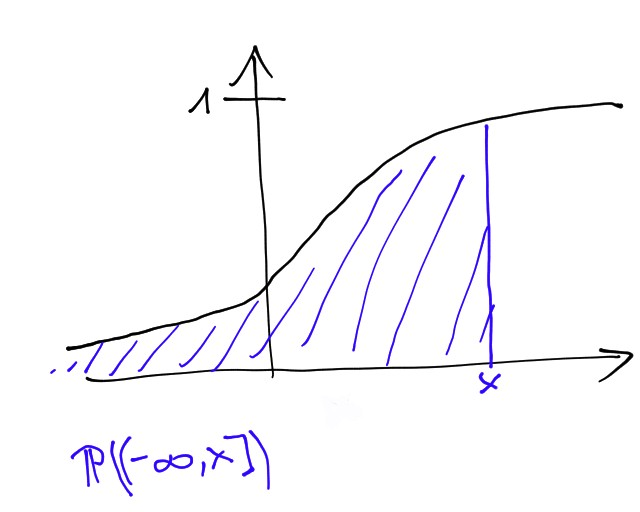
\includegraphics[scale=0.4]{bild.jpg}
		\end{center}
	\end{enumerate}
\end{proof}

\section{Existenz- und Eindeutigkeitssatz}
Sei $F \colon \R \rightarrow [0,1]$ eine Verteilungsfunktion, d.h.
es gelte (1)-(3). Dann existiert genau ein Wahrscheinlichkeitsmaß $\Prim$ auf $\mathcal{B}^1$ mit
$$F(x) = \Prim((- \infty, x]), \quad x \in \R.$$

\begin{proof}
	WT.
\end{proof}

\section{Satz}
Sei $F$ Verteilungsfunktion eines Wahrscheinlichkeitsmaßes $\Prim$ auf $\mathcal{B}^1.$
\begin{enumerate}
	\item $\Prim((a,b]) = F(b) - F(a), \quad a \leq b$
	\item $\Prim(\{x\}) = F(x) - F(\underbrace{x-}_{\text{linksseitiger Grenzwert}})$
	\item $\Prim(\{x\}) = 0 \Leftrightarrow$ $F$ ist stetig in $x$
	\item $F$ besitzt höchstens abzählbar unendlich viele Unstetigkeitsstellen.
\end{enumerate}

\begin{proof}
	\begin{enumerate}
		\item Für $a \leq b$ gilt $(- \infty, a] \cup (a,b] = (- \infty, b]$ also
		$$F(a) + \Prim((a,b]) = F(b).$$
		\item Sei $x_n \uparrow x$ mit $x_n < x$. Dann
		$$(- \infty, x) = \bigcup\limits_{n=1}^\infty{(- \infty, x_n]}$$
		also
		$$\Prim((- \infty, x)) = \lim\limits_{n \rightarrow \infty}{F(x_n)} = F(x-)$$
		Damit
		$$F(x) - F(x-) = \Prim((- \infty, x]) - \Prim((- \infty, x))$$
		$$= \Prim((- \infty, x] \backslash (- \infty, x)) = \Prim(\{x\}).$$
		\item klar.
		\item $\{x \colon F(x) \neq F(x-) \} \subset \bigcup\limits_{n = 1}^{\infty}{ \underbrace{\{x \colon \Prim(\{x\}) \geq \frac{1}{n} \}}_{\text{hat höchstens $n$ Punkte}}}$
	\end{enumerate}
\end{proof}

\section{Beispiel}
Sei $\Prim$ \underline{diskretes Wahrscheinlichkeitsmaß} auf $\mathcal{B}^1$ mit \underline{Träger}
$$T = \{ t_1, t_2, t_3, \ldots \},$$
d.h. $\Prim(\{t_j\}) > 0, \sum\limits_{j=1}^\infty{\Prim(\{t_j\})} = 1$
\newline
Dann gilt (nach Definition)
$$F(x) = \sum\limits_{j \colon t_j \leq x}{\Prim(\{t_j\})}$$
\begin{center}
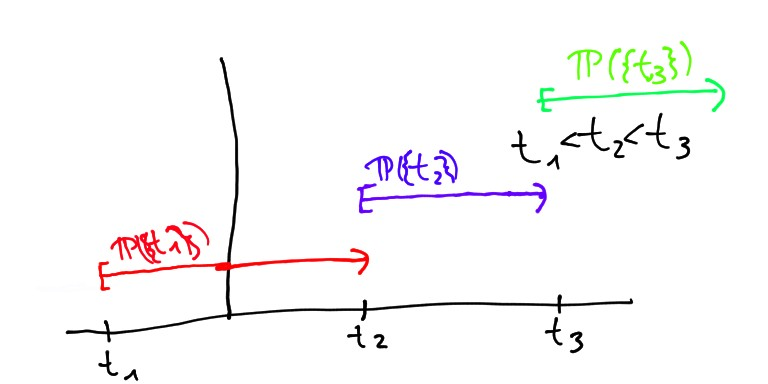
\includegraphics[scale=0.4]{bild2.jpg}
\end{center}

\section{Beispiel}
$$F(x) = \begin{cases} 0, & x \leq 0 \\ x, & 0 \leq x \leq 1 \\ 1, & x \geq 1. \end{cases}$$
\begin{center}
	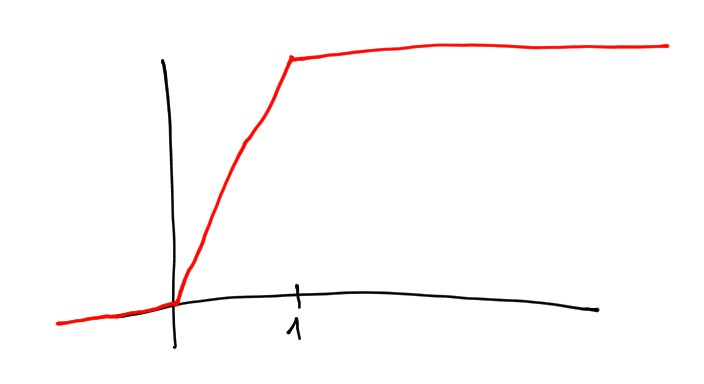
\includegraphics[scale=0.4]{bild3.jpg}
\end{center}

Das zugehörige Wahrscheinlichkeitsmaß $\Prim$ auf $\mathcal{B}^1$ heißt \textbf{Gleichverteilung} auf $[0,1]$ ($\Prim = U([0,1])$). Der Wahrscheinlichkeitsraum
$(\R, \mathcal{B}^1, \Prim)$ modelliert einen "rein zufälligen" Punkt in $[0,1]$.

\section{Definition}
$f \colon \R \rightarrow \R$ heißt \textbf{(Lebesque)Dichte} (über $\R$), falls
\begin{enumerate}
	\item $f(x) \geq 0, x \in \R$
	\item $\{x \colon f(x) \geq c\} \in \mathcal{B}^1, c \in \R$. ($f$ ist Borel-messbar)
	 \item $\int\limits_{- \infty}^{+ \infty}{f(x) dx} = 1$ (Lebesque-Integral)
\end{enumerate}
Die durch 
$$F(x) := \int\limits_{- \infty}^{x}{f(y) dy}, x \in \R$$
definiterte Funktion $F \colon \R \rightarrow [0,1]$ ist stetig und ist eine Verteilungsfunktion im Sinne von 18.9(1),(2),(3). Das nach 18.10 zu $F$ gehörende Wahrscheinlichkeitsmapß $\Prim$ auf $\mathcal{B}^1$ erfüllt
$$\Prim(a,b]) = \int\limits_{a}^{b}{f(y)dy}$$
\begin{center}
	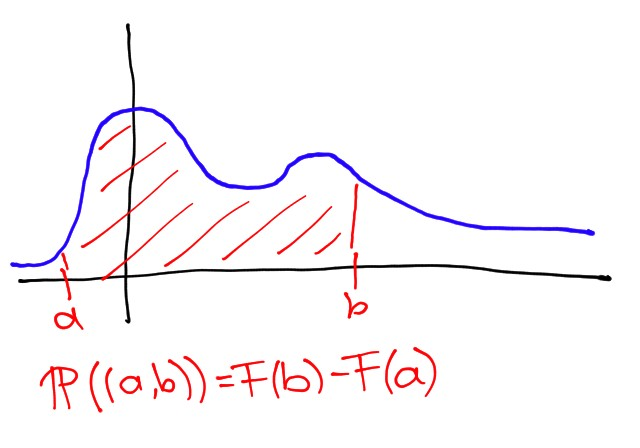
\includegraphics[scale=0.4]{bild4.jpg}
\end{center}
Ist $f$ in $x$ stetig, dann ist $F$ in $x$ stetig differenzierbar und $F^\prime(x) = (x)$.

Das bedeutet 
$$"\Prim((x, x+dx]) \approx f(x) dx"$$

(TODO: Rest texen)

\section{Beispiel} %18.19
Seien $f_1, \ldots, f_k$ Dichten auf $\R$. Setze
$$f(x_1, \ldots, x_k) = \prod\limits_{j=1}^k{f_j(x_j)}, \quad x_1, \ldots, x_k \in \R$$
Diese Funktion ist messbar und
$$\int{f(x) dx} = \int \ldots \int f_1(x_1) \ldots f_k(x_k) dx_1 \ldots d x_k = \prod\limits_{j=1}^k{\int f_j(x_j) dx_j} = 1$$

\section{Beispiel} %18.20
$f_j(t) = f(t) = \frac{1}{\sqrt{2 \pi}} exp[-\frac{t^2}{2}]$
\newline
Dann ist
$$f(x_1, \ldots, x_k) = \prod\limits_{j=1}^k{f_j(x_j)} = \frac{1}{(2 \pi)^{\frac{k}{2}}} exp[-\frac{1}{2} \sum\limits_{j=1}^k{x_j^2}]$$ die Dichte der k-dimensionalen Normalverteilung.

\section{Definition und Bemerkung}
Sei $\Prim$ ein Wahrscheinlichkeitsmaß auf $\R^k$. Für $j \in \{1, \ldots, k\}$ sei
$$\Prim_j(B) := \Prim(\R^{j-1} \times B \times \R^{k-j}), B \in \mathcal{B}^1$$
Das ist ein Wahrscheinlichkeitsmaß. Man nennt es $j$-te Randverteilung von $\Prim$. Hat $\Prim$ die Dichte $f$, so hat $\Prim_j$ die Dichte 
$$f_j(t) = \int \ldots \int f(x_1, \ldots, x_{i-1}, t, x_{i+q}, \ldots, x_k) d x_1 \ldots d x_{j-1} \ldots d x_k$$ (Fubini)

\chapter{Zufallsvariablen}
Sei $(\Omega, \mathcal{A}, \Prim)$ Wahrscheinlichkeitsraum.
\newline
Früher: $X \colon \Omega \rightarrow \R, \Prim^X(B) := \Prim(X^{-1}(B))$

\section{Definition und Satz}
Sei $\Omega^\prime \neq \emptyset, \mathcal{A}^\prime \subset \mathcal{P}(\Omega^\prime)$ $\sigma$-Algebra.

Eine Abbildung $X \colon \Omega \rightarrow \Omega^\prime$ heißt \textbf{$(\mathcal{A}, \mathcal{A}^\prime)$-messbar}, falls
$$X^{-1}(B) \in \mathcal{A}, \quad B \in \mathcal{A}^\prime.$$
Dann heißt $X$ \textbf{$\Omega^\prime$-wertige Zufallsvariable}.

Die Verteilung 
$\Prim^{X} (\Prim (X_{\ldots}), \mathcal{L}(x), \Prim X^{-1}, \ldots)$ von $X$ ist definiert als
$$\Prim^X(B):= \Prim(X^{-1}(B)), B \in \mathcal{A}^\prime$$
Das ist ein Wahrscheinlichkeitsmaß auf $(\Omega^\prime, \mathcal{A}^\prime)$.
(ÜA). Ist $(\Omega^\prime, \mathcal{A}^\prime) = (\R^k, \mathcal{B}^k)$, nennt man $X$ einen $k$-dimensionalen Zufallsvektor. Im Fall $k=1$ spricht man von einer Zufallsvariable.

\section{Bemerkung}

\begin{enumerate}
	\item Sei $\mathcal{M}^\prime \subset \mathcal{A}^\prime$ mit $\sigma(\mathcal{M}^\prime) = \mathcal{A}^\prime$. Dann gilt
$$X^{-1}(A^\prime) \in \mathcal{A}^\prime, A^\prime \in \mathcal{M}^\prime \Leftrightarrow X^{-1}(A^\prime) \in \mathcal{A}^\prime, A^\prime \in \mathcal{U}^\prime.$$
Zu zeigen ist ($\Rightarrow$). Setze
$$\mathcal{G}:= \{ A ^\prime \subset \Omega^\prime \colon X^{-1}(A^\prime) \in \mathcal{A} \}$$
Das ist eine $\sigma$-Algebra (ÜA). \newline

Also gilt (wegen $\mathcal{M}^\prime \subset \mathcal{G}$)
$$\mathcal{A}^\prime = \sigma(\mathcal{M}^\prime) \subset \sigma(\mathcal{G}) = \mathcal{G}$$
	\item Sei $g \colon \R^k \rightarrow \R^l$ stetig.
	Dann gilt
	$$g^{-1}(A^\prime) \in \mathcal{O}^k \subset \mathcal{B}^k, A^\prime \in \mathcal{O}^l$$
	Wegen $\sigma(\mathcal{O}^l) = \mathcal{B}^l$ folgt aus (i)
	$$g^{-1}(A^\prime) \in \mathcal{B}^k, A^\prime \in \mathcal{B}^l.$$
	Also ist $g$ messbar.
	
	\item $g \colon \R^k \rightarrow \R$ messbar (d.h. $(\mathcal{B}^k, \mathcal{B}^1)$-messbar) $\Leftrightarrow$
	$$\{x \colon g(x) \geq c \} \in \mathcal{B}^k.$$
	\begin{proof}
		Das System
		$$\{[c, \infty) \colon c \in \R\}$$
		ist ein Erzeuger von $\mathcal{B}^1$.
		\newline
		Man benutze jetzt $(i)$.
	\end{proof}
	\item Sei $X \colon \Omega \rightarrow \Omega^\prime$ $(\mathcal{A}, \mathcal{A}^\prime)$-messbar. \newline
	Sei $h \colon \Omega^\prime \rightarrow \Omega^{\prime\prime}$ $(\mathcal{A}^\prime, \mathcal{A}^{\prime\prime})$-messbar, wobei $\mathcal{A}^{\prime\prime} \subset \mathcal{P}(\Omega^{\prime\prime})$ eine $\sigma$-Algebra ist.
	\newline
	Dann ist die Abbildung $h \circ X \colon \Omega \rightarrow \Omega^{\prime\prime}$ $(\mathcal{A}, \mathcal{A}^{\prime\prime})$-messbar. Für $A^{\prime\prime} \in \mathcal{A}^{\prime\prime}$
	$$(h \circ X)^{-1}(A^{\prime\prime}) = X^{-1}(\underbrace{h^{-1}(A^{\prime\prime})}_{\in \mathcal{A}^\prime}) \in \mathcal{A}.$$
	\item Sei $\mathcal{D}$ ein Wahrscheinlichkeitsmaß auf $(\R^k, \mathcal{B}^k)$. Dann existiert ein Wahrscheinlichkeitsraum $(\Omega, \mathcal{A}, \Prim)$ mit $\Prim^X = \mathcal{D}$.
	\newline
	Dazu: $(\Omega, \mathcal{A}, \Prim) = (\R^k, \mathcal{B}^k, \mathcal{D})$,
	$$X = id_{\R^k}$$ 
\end{enumerate}

%31.01.12
\paragraph{Erinnerung}
$(\Omega, \mathcal{A}, \Prim) \quad X \colon \Omega \rightarrow \Omega^\prime$
$\mathcal{A}^\prime$

\paragraph{Messbarkeit:}
$X^{-1}(B) \in \mathcal{A}, B \in \mathcal{A}^\prime$ \newline
$\Prim^X$ Wahrscheinlichkeitsmaß auf $(\Omega^\prime, \mathcal{A}^\prime)$
$$\Prim^X(B) = \Prim(X^{-1}(B)) =: \Prim(X \in B)$$ ($= \Prim(\{X \in B\}) = \Prim(\{ \omega \in \Omega \colon X(\omega) \in B\})$) \newline

$\Omega^\prime = \R^k \quad \mathcal{B}^k$ Zufallsvektor
\newline
$k=1$ Zufallsvariable

\section{Bemerkung}
Sei $\Q$ Wahrscheinlichkeitsmaß auf $\R^k$. \newline
$X \colon \Omega \rightarrow \R^k$ mit Verteilung $\Q$.
Man schreibt
$$X \sim \Q$$ ("$X$ ist nach $\Q$ verteilt.") \newline

\underline{z.B.:} $X \sim U[a,b]$ \footnote{$X$ auf dem Intervall $[a,b]$ gleichverteilt.} \newline
$X \sim Exp(\lambda), X \sim N(\mu, \sigma^2)$
\newline
Hat $\Q$ die Dichte $f$, so sagt man "$X$ hat Dichte $f$". \newline
Man sagt $X$ ist eine (absolut) stetige Zufallsvariable. \footnote{Das bedeutet: $X$ hat eine Dichte.}
\newline
$$\Prim(a \leq X \leq b) = \int\limits_a^b{f(x)dx}, \quad a \leq b$$
$$\Prim(X = t) = 0!$$

\section{Bemerkung}
Sei $\mathcal{Q}^k := \{ [a,b] \colon a \leq b \}$ \footnote{$a,b \in \R^k$} \newline
Für $\lambda^k([a,b]) := \prod\limits_{j=1}^k{(b_j - a_j)}$ \footnote{Lebesque-Maß}

$N \in \mathcal{B}^k$ heißt \textbf{Nullmenge}
$$\Leftrightarrow \forall \epsilon > 0 \quad \exists k_1, k_2, \ldots \in \mathcal{Q}^k$$
mit $N \subset \bigcup\limits_{i=1}^{\infty}{k_i}$ und $\sum\limits_{j=1}^{\infty}{\lambda^k(k_j)} \leq \epsilon$.

(Hyperebenen $\{ x \colon <x,n> = c \}$ sind Nullmengen) \newline

Sind $f,g \colon \R^k \rightarrow \R$ Dichten eines Wahrscheinlichkeitsmaßes $\Q$, so gilt
$$f(x) = g(x), \quad x \notin N,$$
mit einer Nullmenge $N$.

\section{Bemerkung}
Hat ein $k$-dimensionaler Zufallsvektor die Dichte $f$, so hat die
$X_j$ die Dichte
$$f_j(t)= \int \ldots \int f(x_1, \ldots, x_{j-1}, t, x_{j+1}, \ldots, x_k) dx_1 \ldots dx_k$$

\section{Beispiel}
$(X,Y)$ habe Dichte 
$$f(x,y) := \frac{1}{\pi} 1_{\{x^2 + y^2 \leq 1\}} \equiv 1_K(x,y), K = \{(x,y) \colon x^2 + y^2 \leq 1\} )$$
Dann
$$f_1(x) = \int{f(x,y) dy} = \int 1_{\{x^2 + y^2 \leq 1\}} dy = \int 1_{\{|y| \leq \sqrt{1-x^2}\}} dy$$
$$= \begin{cases} 0, & \text{ falls } |x| > 1 \\ \frac{2}{\pi} \sqrt{1-x^2}, & \text{ falls } |x| \leq 1 \end{cases}$$

\begin{center}
	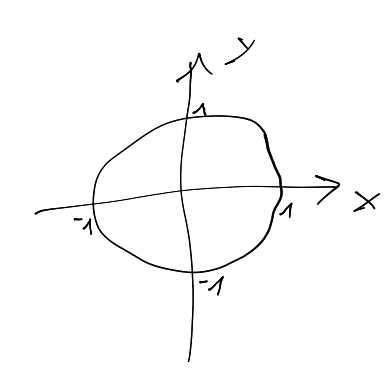
\includegraphics[scale=0.3]{kreis.jpg}
\end{center}

Ferner
$$F_X(t) = \Prim(X \leq t) = \int\limits_{-\infty}^t{f_1(x) dx} = \int\limits_{-1}^t{\frac{2}{\pi} \sqrt{1-x^2} dx}, \quad -1 \leq t \leq 1$$
$$\overset{!}{=} \frac{1}{2} + \frac{1}{\pi} \arcsin(t) + \frac{1}{\pi} t \sqrt{1-t^2}$$
(Differentiation und $\frac{\partial}{\partial t} \arcsin(t) = \frac{1}{\sqrt{1-t^2}}$)
\begin{center}
	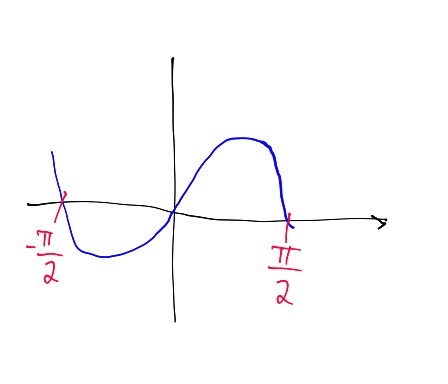
\includegraphics[scale=0.3]{sinus.jpg}
\end{center}

\section{Definition}
\begin{enumerate}
	\item \footnote{Die Ereignisse} $A_1, \ldots, A_n \in \mathcal{A}$ heißen \textbf{stochastisch unabhängig}, falls 
	$$\Prim(\bigcap\limits_{j \in T}{A_j}) = \prod\limits_{j\in T}{}\Prim(A_j), \quad T \subset \{1, \ldots, n\}, T \neq \emptyset$$
	\item Zufallsvariablen $X_1, \ldots, X_n$ heißen \textbf{stochastisch unabhängig}, falls
	$$X_1^{-1}(B_1), \ldots, X_n^{-1}(B_n) \text{ stochastisch unabhängig, für alle } B_1, \ldots, B_n \in \mathcal{B}^1,$$
	bzw. falls
	$$\Prim(X_1 \in B_1, \ldots X_n \in B_n) = \prod\limits_{j=1}^n{\Prim(X_j \in B_j)} \text{ für alle } B_1, \ldots, B_n \in \mathcal{B}^1.$$
\end{enumerate}

\section{Bemerkung}
Hat $(X_1, \ldots, X_n)$ die Dichte $f$. Dann gilt:
\begin{enumerate}
\item $f(x) = \prod\limits_{j=1}^{n}{f_j(x_j)} \Rightarrow X_1, \ldots, X_n \text{ stochastisch unabhängig}$
\item $X_1, \ldots, X_n \text{ stochastisch unabhängig } \Rightarrow f(x) = \prod\limits_{j=1}^n{f_j(x_j)} \text{ außerhalb einer Nullmenge}$
\end{enumerate}


\begin{proof}
	$(1): $
	
	$$\Prim((X_1, \ldots, X_n) \in B_1 \times \ldots \times B_n)$$
	$$= \Prim^X(B_1 \times \ldots \times B_n) = \int\limits_{B_1 \times \ldots \times B_n}{f(x)dx}$$
	$$\overset{(1), Fubuni}{=} \int\limits_{B_1} \int\limits_{B_2} \ldots \int\limits_{B_n}{ f(x_1) \ldots f(x_n) dx_n \ldots dx_1}$$
	$$= \prod\limits_{j=1}^n{\int\limits_{B_j}{f_j(x)dx}} = \prod\limits_{j=1}^n{\Prim^{X_j}(B_j)} = \prod\limits_{j=1}^n{\Prim(X_j \in B_j)}$$
	
	$(2): $
	WT
\end{proof}

\chapter{Rechnen mit Dichten}
$X = (X_1, \ldots, X_k)$ $k$-dimensionaler Zufallsvektor mit Dichte $f$. Sei 
$$T \colon \R^k \rightarrow \R^s \quad (s \leq k)$$
Sei $Y := T(X)$.
($Y$ ist $s$-dimensionaler Zufallsvektor, falls $T$ messbar ist.)

\section{Satz}
Sei $K=1$, d.h. $X$ sei reelle Zufallsvariable. Die Dichte $f$ sei stückweise stetig und es gelte 
$$\Prim(X \in I) = 1$$
für ein offenes Intervall $I \subset \R$. Die Einschränkung $T \big |_I$ (von $T$ auf $I$) sei stetig differenzierbar, streng monoton und $T^\prime(x) \neq 0, x \in I$.
Dann hat $Y=T(X)$ die Verteilungsfunktion
$$G(y) = \begin{cases} F(T^{-1}(y)), y \in T(I), & \text{ falls } T \uparrow \\
1-F(T(y)), y \in T(I), & \text{ falls } T \downarrow \end{cases}$$
wobei $F$ die Verteilungsfunktion von $X$ ist. Ferner hat
$G$ die Dichte
$$g(y) = \frac{f(T^{-1}(y))}{|T^\prime(T^{-1}(y))|}, \quad y \in T(I)$$
und $g(y) = 0$ für $y \notin T(I)$.

\begin{proof}
	Sei $T$ wachsend. Dann
	$$G(y) = \Prim(Y \leq y) = \Prim(T(X) \leq y)$$
	$$= \Prim(X \leq T^{-1}(y)) \quad y \in T(I)$$
	Die Funktion $G$ ist stetig differenzierbar mit Ableitung 
	$$g(y) = G^\prime(y) = \frac{f(T^{-1}(y))}{T^\prime(T^{-1}(y))}$$
\end{proof}

\section{Beispiel}
$T(x) = ax+b, \quad a \neq 0, b \in \R$ \newline
$T^\prime(x) = a, T^{-1}(y) = \frac{y-b}{a}$ \newline
$g(y) = \frac{1}{|a|} f(\frac{y-b}{a})$

\section{Beispiel}
$X \sim N(0,1)$ \footnote{Normalverteilung mit Mittelwert 0 und Standardabweichung 1},
$T(x) = \sigma x + \mu$ ($\sigma > 0, \mu \in \R$), $Y:= T(X) = \sigma X+\mu$

$$g(y) = \frac{1}{\sigma} \varphi(\frac{y-\mu}{\sigma}) = \frac{1}{\sqrt{2 \pi \sigma^2}} \exp [- \frac{(y-\mu)^2}{\sigma^2}]$$ \footnote{$\varphi$ ist die Dichte der Standardnormalverteilung}

\section{Beispiel}
$T(x) = x^2, Y = X^2$
$$G(y) = \Prim(Y \leq y)$$
$$= \Prim(X^2 \leq y)$$
$$\overset{y \geq 0}{=} \Prim(- \sqrt{y} \leq X \leq \sqrt{y})$$
$$= F(\sqrt{y}) - F(-\sqrt{y})$$
\footnote{$F$ ist die Verteilungsfunktion von $X$.}
Dichte ($y>0$):
$$g(y) = f(\sqrt{y}) \cdot \frac{1}{2 \sqrt{y}} + f(-\sqrt{y}) \cdot \frac{1}{2 \sqrt{y}}$$

%07.02.2012
\paragraph{Erinnerung}
$f \colon \R^k \rightarrow \R$ Dichtefunktion von $X = (X_1, \ldots, X_k)$
\newline
$Y=T(X)$ \footnote{Transformation von $X$}
\newline
$\Prim(X \notin U) = 0 = \int\limits_{U^c}{f(x) dx}$
\section{Satz}
Sei $U:= \{x \in \R^k \colon f(x) > 0 \}$ offen, $V \subset \R^k$ offen, $T \colon U \rightarrow V$ bijektiv, stetig differenzierbar,
$T^\prime(x) \neq 0, \quad x \in U$. Dann hat $Y:=T(X)$ die Dichte
$$g(y) = \frac{f(T^{-1}(y))}{|\det T^{\prime}(T^{-1}(y))|}, \quad y \in V$$
$(g(y) = 0, \quad y \notin V.)$

\begin{proof}
zu zeigen:
$$\Prim(Y \in B) = \int\limits_B{f(y) dy, \quad B \in \mathcal{B}^k} \qquad (*)$$
Wir zeigen $(*)$ für offenes $B \subset V$. (Das genügt!) \footnote{siehe Maßtheorie} Dann
$$\Prim(Y \in B) = \Prim(X \in T^{-1}(B))$$
$$= \int\limits_{T^{-1}(B)}{f(x) dx} \qquad | x = T^{-1}(y), y = T(x)$$
$$= \int\limits_B{f(T^{-1}(y) \left(\det T^\prime(T^{-1}(y))\right)^{-1} dy}$$
Analysis 3! \footnote{Jacobi-Determinante}
\end{proof}

\section{Beispiel (Polarmethode)}
Seien $X_1, X_2$ stochastisch unabhängig und $U(0,1)$-verteilt.
Dann $f(x_1, x_2) = 1_{(0,1)^2}(x_1, x_2)$
Es sei 
$$T(x_1, x_2) = (\sqrt{-2 \log x_1} \cos(2 \pi x_1), \sqrt{-2 \log x_2} \sin(2 \pi x_2))$$
Dann ist $T((0,1)^2) = \R^1 \backslash \{(y_1, y_2) \colon y_1 \geq 0, y_2 = 0 \}.$ (Nullmenge)

$\det T^\prime(x_1, x_2) = \frac{2\pi}{x_1}$ (Übung!)

Aus Satz 20.5 folgt $(x_1 = \exp [-\frac{1}{2}(y_1^2, y_2^2)])$

$$g(y_1, y_2) = (\frac{2 \pi}{\exp [- \frac{1}{2} (y_1^2 + y_2^2)]})^{-1} 1_V(y_1,y_2)$$
$$\overset{!}{=} f(y_1) f(y_2)$$
19.8.(i) $\leadsto Y_1, Y_2$ unabhängig $N(0,1)$-verteilt.

\section{Beispiel}
$T(x) = Ax + b$,

$A \in \R^{k \times k}$ regulär, $b \in \R^k, Y = T(X)$ hat Dichte
$$g(y) = \frac{f(A^{-1}(y-b))}{|\det A|}$$

\section{Bemerkung}
Sei $T \colon \R^k \rightarrow \R^s$ mit $k>s$. Betrachte
$$\widetilde{T} \colon \R^k \rightarrow \R^{s+(k-s)}$$ mit
$$\widetilde{T}(x) = (T_1(x), \ldots, T_s(x), \underbrace{T_{s+1}(x), \ldots, T_k(x)}_{\text{"Auffüllen"}}$$

Erfüllt $\widetilde{T}$ die Voraussetzung von Satz 20.5, dann hat
$$\widetilde{Y} := \widetilde{T}(x)$$
eine Dichte $f_{\widetilde{Y}}$. Wegen
$$Y = (\widetilde{Y_1}, \widetilde{Y_2})$$
folgt , dass $Y$ die Dichte

$$f_Y(y_1, \ldots, y_s) = \int{ \int{f_{\widetilde{Y}}(y_1, \ldots, y_s, y_{s+1}, \ldots, y_k) dy_{s+1} \ldots dy_k}}$$

\section{Beispiel}
$k=2, s=1$
$$Y:= T(X) := X_1 + X_2$$
$$\widetilde{T}(x_1, x_2) := (x_1 + x_2, x_1)$$
Dann hat $\widetilde{T}$ die Jacobi-Determinante 1 und $\widetilde{Y} := (x_1 + x_2, x_2)$ die Dichte $f_{\widetilde{y}}(y_1, y_2) = f(y_2, y_1-y_2) 1$ und damit die Dichte
$$f_{X_1 + X_2} = \int f(y_2, y_1-y_2) dy_2$$
Sind $X_1, X_2$ unabhängig, d.h. $f(x_1, x_2) = f_1(x_1) f_2(x_2)$, dann gilt
$$f_{X_1 + X_2}(z) = \int f_{X_1}(t) f_{X_2}(z-t) dt$$
(Faltungsformel)

$(= f_1 * f_2 (z))$

\section{Satz (Additionsgesetz für Nomalv.)}
Seien $X,Y$ unabhängig, $X \sim N(\mu, \sigma^2), Y \sim N(\nu, \tau^2)$. Dann gilt
$$X + Y \sim N(\mu + \nu, \sigma^2 + \tau^2)$$

\begin{proof}
Seien $U,V$ unabhängig $N(0,1)$-verteilt. Setze
$$\widetilde{X} := \sigma U + \mu, \widetilde{Y} := \tau V + U.$$
Dann sind $\widetilde{X}, \widetilde{Y}$ unabhängig und es gilt
$$(X,Y) \overset{d}{=} (\widetilde{X}, \widetilde{Y}).$$
Damit (!)
$$X+Y \overset{d}{=} \widetilde{X} + \widetilde{Y} = \sigma U + \tau V + \mu + \nu$$
$$= \sqrt{\sigma^2 + \tau^2} (\underbrace{\frac{\sigma}{\sqrt{\sigma^2 + \tau^2}} U + \frac{\tau}{\sqrt{\sigma^2 + \tau^2}} V}_{N(0,1) \text{ ÜA!}}) + (\mu + \nu)$$
Faltungsformel!
\end{proof}

\section{Definition und Satz}
Seien $X_1, \ldots, X_k$ unabhängig $N(0,1)$-verteilt.

Betrachte $Y:= X_1^2 + \ldots + X_k^2.$ Die Verteilung von $Y$ heißt
\textbf{$\chi^2$-Verteilung} mit $k$ \textbf{Freiheitsgraden} (kurz $Y \sim \chi^2_k$). $Y$ hat die Dichte
$$f_k(x) = \frac{1}{2^{\frac{k}{2}} \Gamma(\frac{k}{2})} x^{\frac{k}{2}-1} e^{-\frac{x}{2}}, \quad x > 0.$$

\paragraph{Beweisidee:}
$\Gamma(\alpha) = \int\limits_0^{\infty}{x^{\alpha-1} e^{-x} dx}, \quad \alpha > 0.$
($\Gamma(k) = (k-1)!$).

Man beweist zunächst den Fall $k=1$ (Transformationsformel).

Der allgemeine Fall folgt induktiv mit Faltungsformel. Allgemeiner gilt ein Additionsgesetz für Gammaverteilungen (siehe Übungsblatt).

\chapter{Kenngrößen von Verteilungen}

\paragraph{Erinnerung:}
$(\Omega, \Prim)$ diskreter Wahrscheinlichkeitsraum

$X \colon \Omega \rightarrow \R$

\begin{enumerate}
	\item $\E X := \sum\limits_{\omega \in \Omega} X(\omega) \Prim(\{\omega\})$
	\item $= \sum\limits_{X \colon \Prim(X=x) > 0} x \Prim(X=x)$
\end{enumerate}

\paragraph{Jetzt:}
$(\Omega, \mathcal{A}, \Prim)$ Wahrscheinlichkeitsraum, $X \colon \Omega \rightarrow \R$ Zufallsvariable.

\paragraph{Ziel:} Definition von $\E X$!

\begin{enumerate}
	\item $X \geq 0$. Für $n \in \N$ sei 
	$$X_n(\omega) := \begin{cases} 0, & \text{falls } X(\omega)=0 \\ \frac{j-1}{2^n}, & \text{falls } \frac{j-1}{2^n} < X \leq \frac{j}{2^n}, j=1, \ldots, n 2^n \\
	n, & \text{falls } X(\omega) > n. \end{cases}$$
	Es gilt \footnote{Linke Intervallgrenze als Approx} $X_n(\omega) \leq X_{n+1}(\omega), \lim\limits_{n \rightarrow \infty}{X_n(\omega) = X(\omega)}$, und wir definieren
	
	$$\E X_n := \sum\limits_{j=1}^{n 2^n}{\frac{j-1}{2^n} \left(F\left(\frac{j}{2^n}\right) - F\left(\frac{j-1}{2^n}\right)\right)} + n (1-F(n))$$ \footnote{$F$ Verteilungsfkt.}, wobei $F(x):= \Prim(X \leq x)$. (Motivation kommt von (2).)
	
	Es gilt 
	$$\E X_n \leq \E X_{n-1}$$ und wir definieren:
	$$\E X := \lim\limits_{n \rightarrow \infty} \E X_n \in [0, \infty].$$
	Erwartungswert von $X$ ($\E X = \int X d \Prim$).
	
	\item $X$ beliebig. Dann gilt
	$$X = X^+ - X^-$$
	mit $X^+ := \max \{X,0\}, X^- := - \min \{X,0\}$
	
	(Es gilt $|X| = X^+ + X^-$.)
\end{enumerate}

\section{Definition}
$X$ ist \textbf{integrierbar}, wenn $\E X^+ < \infty$ und $\E X^- < \infty$. In diesem Fall sei $\E X := \E X^+ - \E X^- \left(= \int X d \Prim = \int X(\omega) d \Prim(\omega) = \int X(\omega) \Prim(d \omega)\right)$

\section{Satz}
Besitzt $X$ eine Dichte $f$, dann ist $X$ genau dann integrierbar, wenn
$$\int |x| f(x) dx < \infty.$$
Dann gilt
$$\int x f(x) dx = \E X.$$

\end{document}
